\chapter{User documentation}
\label{ch:user}

This chapter is dedicated for the potential users. In \autoref{sec:GeneralRequisite}, the requisite of opening and using the application is listed. It also gives an introduction to the types of user roles within the solution, to enable the users to navigating through the thesis and find their related information quickly.

Then in the following sections (\autoref{sec:UdocEndUser}, \autoref{sec:UdocReceptionist}, \autoref{sec:UdocFacilityManager}, \autoref{sec:UdocAdministrator}), which are titled by the roles, collects the use guide of each accessible applications.

\section{General Requisite}
\label{sec:GeneralRequisite}

The solution is for the internal usage within SAP for the parcel collection service providing to the employees. The solution consists of 6 applications as tiles on the Fiori launchpad \cite{flp}: \textbf{My packages}, \textbf{Pickup packages}, \textbf{Register Packages}, \textbf{Manage packages}, \textbf{Manage Companies} and \textbf{Manage Storages} partitioned into 3 sections: \textbf{My Home}, \textbf{Pacel Handling}, \textbf{Administration}, as shown in \autoref{fig:ApplicationLaunchScreen}.

\begin{figure}[H]
	\centering
	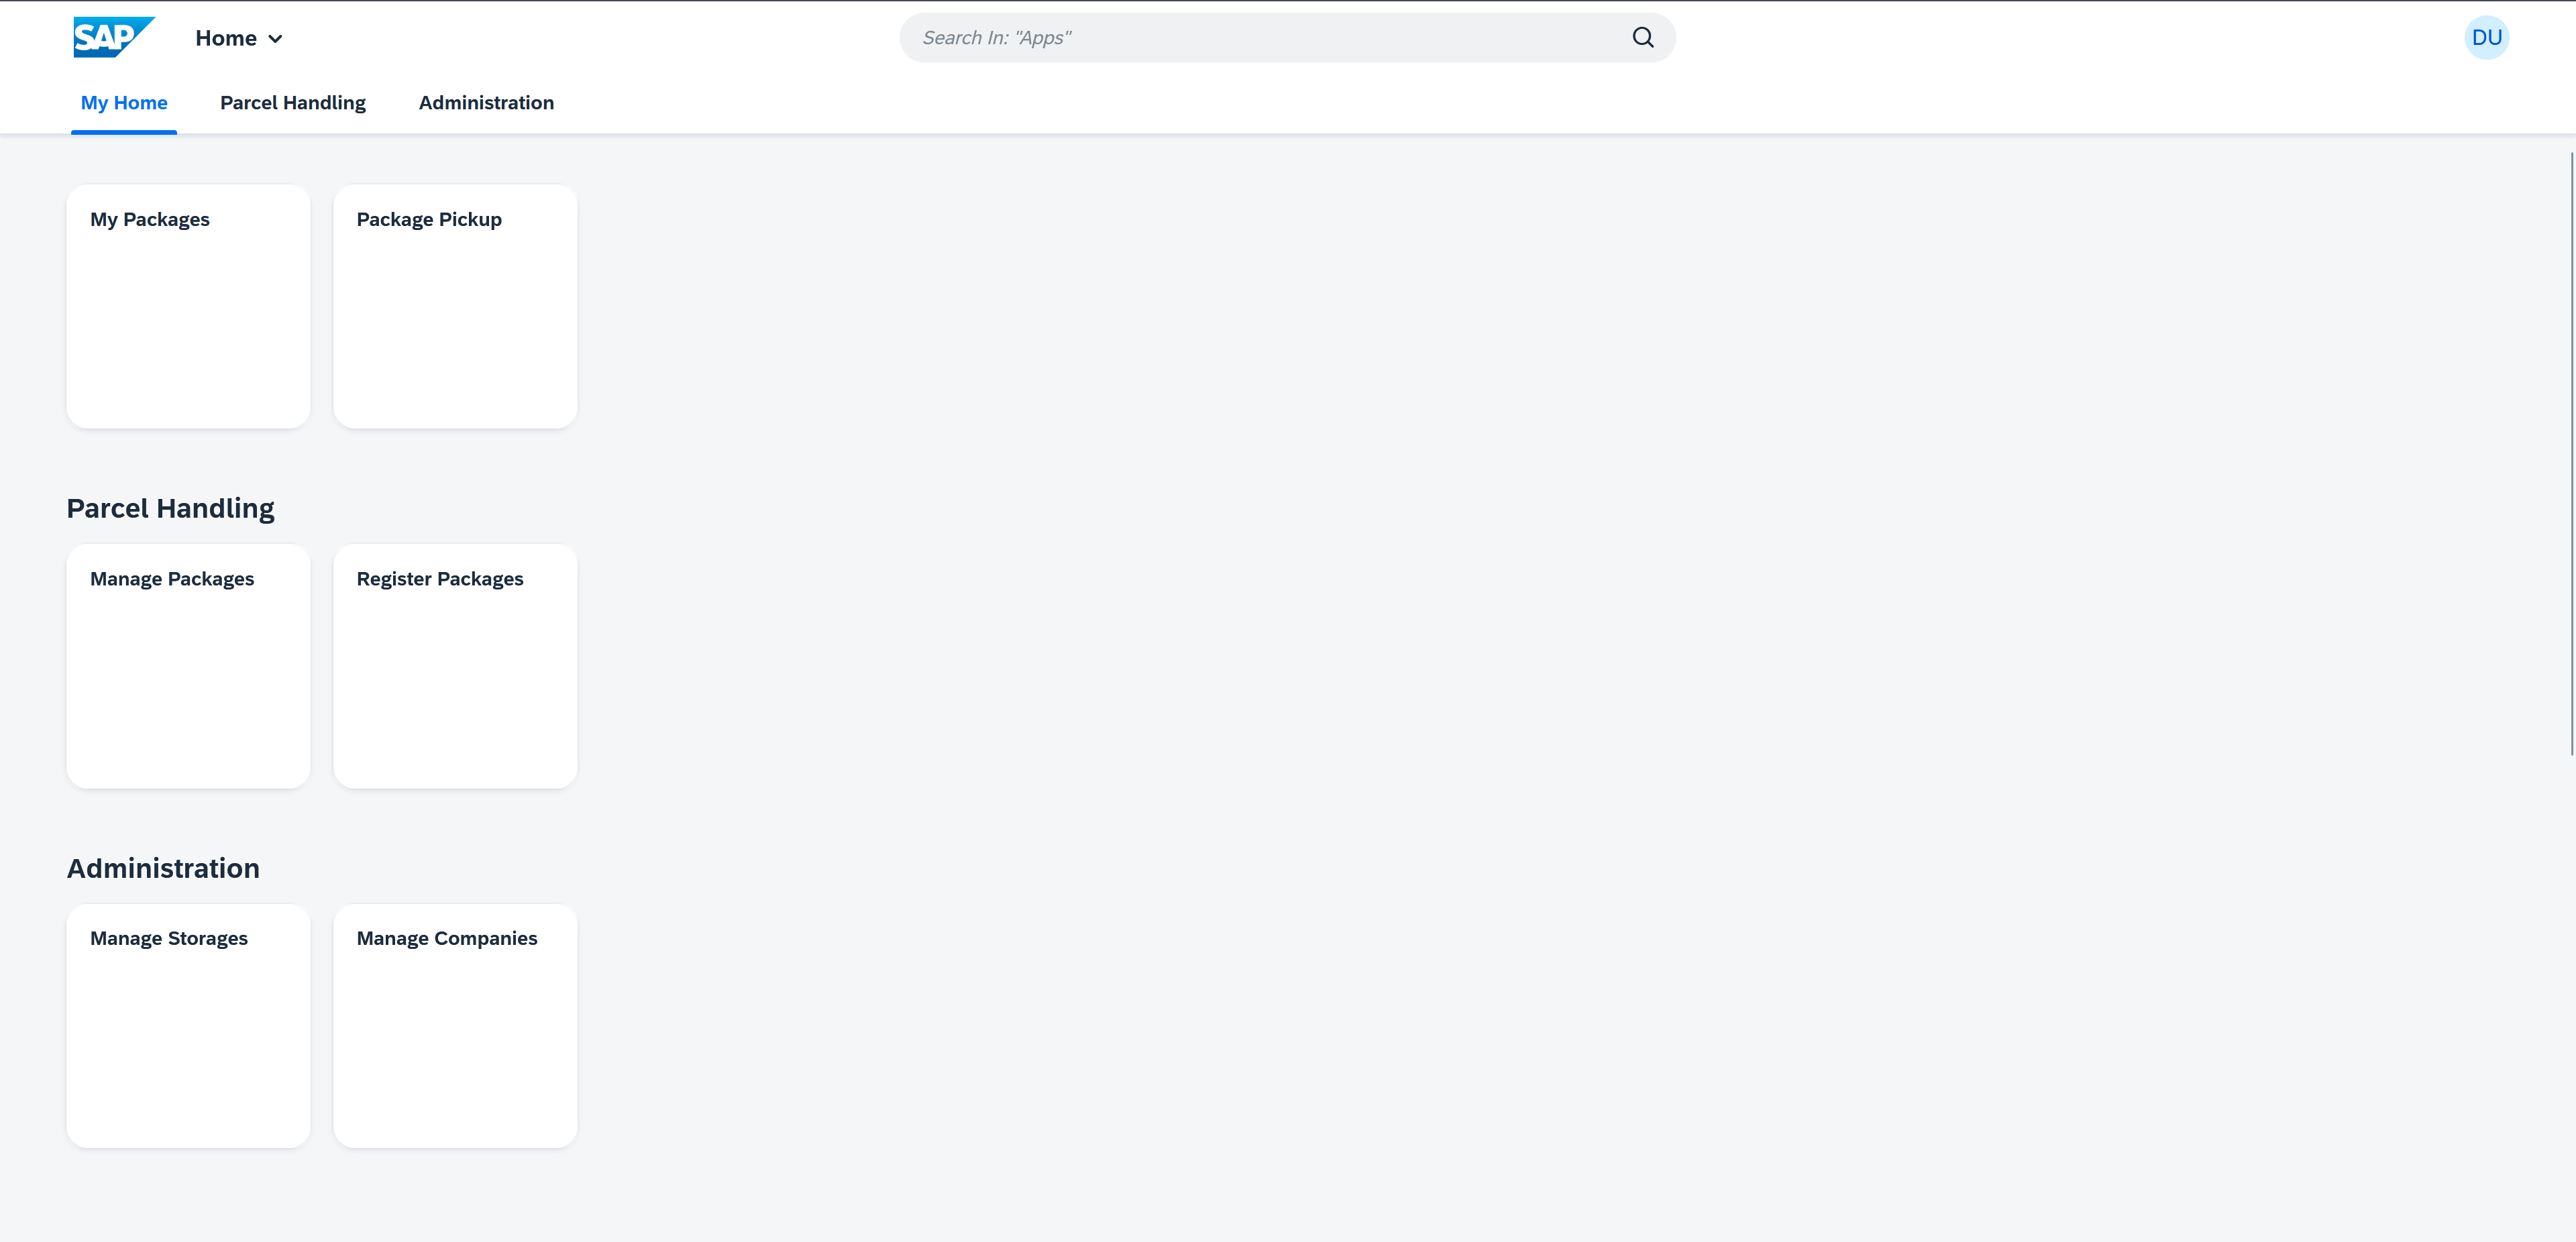
\includegraphics[width=1\linewidth]{images/user_doc/overviews/sandbox.png}
	\caption{Application Launch Screen}
	\label{fig:ApplicationLaunchScreen}
\end{figure}


In order to use any of the application, one has to hold an SAP registered device (computer/tablet/phone) and is able to use a supported browser with stable internet connection. In order to use \textbf{Pickup packages} application, one has to hold an SAP registered smart phone. 

In order to mock use the application in local environment, please move the the developer documentation (\autoref{ch:impl}) and follow the set up steps. 

Four different roles are specified for the application and an authenticated user is limited to applications dedicated to their assigned roles. In the coming sections the usage guides are documented sectioned by the roles. Hereby lists the meaning of each role under the thesis context and feel ease to jump to the related section by clicking section links.

\begin{description}
	\item[End User (\autoref{sec:UdocEndUser})] Any SAP employee who holds an SAP registered device and would like to use the parcel collection service.
	\item[Receptionist (\autoref{sec:UdocReceptionist})] Registered receptionist working at the reception and is responsible to serve the parcel collection service. Assigned "Receptionist" role on BTP.
	\item[Facility Manager (\autoref{sec:UdocFacilityManager})] Authorised user who is responsible for maintaining the delivery companies and storage slots information. Assigned "FacilityManager" role on BTP.
	\item[Administrator (\autoref{sec:UdocAdministrator})] The master user who can access to any of the applications. Assigned "Administrator" role on BTP.
\end{description}

In case one is accessing the applications through browser from BTP platform \cite{btp}, the login process is done automatically. Otherwise, if one is running the application locally, a browser pop up will appear (\autoref{fig:LocalLoginPopUp}) and mock user (See existing mock credentials in \autoref{sec:D-security}) should be entered.
In the case of any user trying to accessing an unauthorised application, connection will fail. (\autoref{fig:IllegalAccesstoUnauthorised Applications})

\begin{figure}[H]
	\centering
	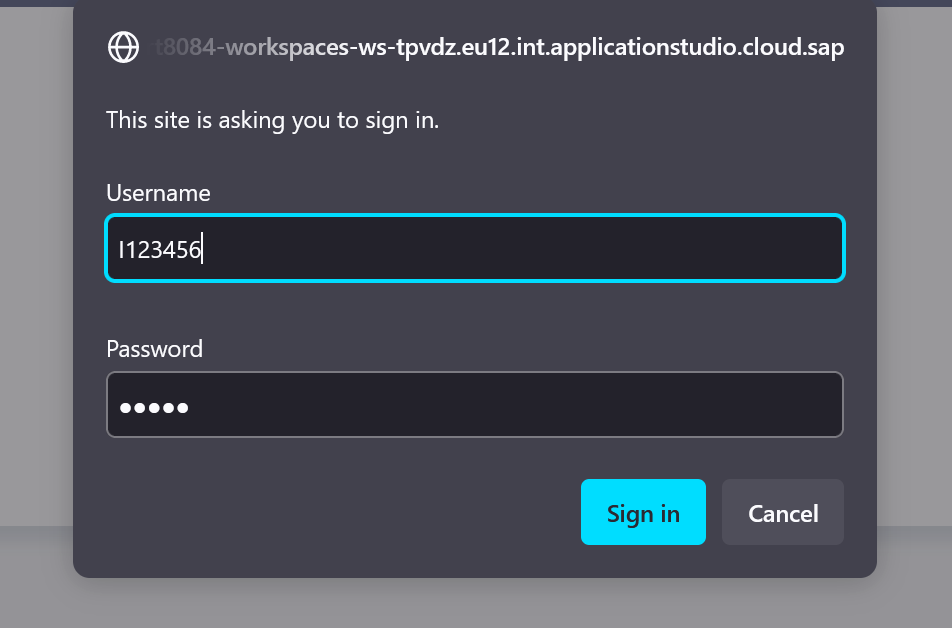
\includegraphics[width=0.5\linewidth]{images/user_doc/overviews/localLogin.png}
	\caption{Local Login Pop Up}
	\label{fig:LocalLoginPopUp}
\end{figure}

\begin{figure}[H]
	\centering
	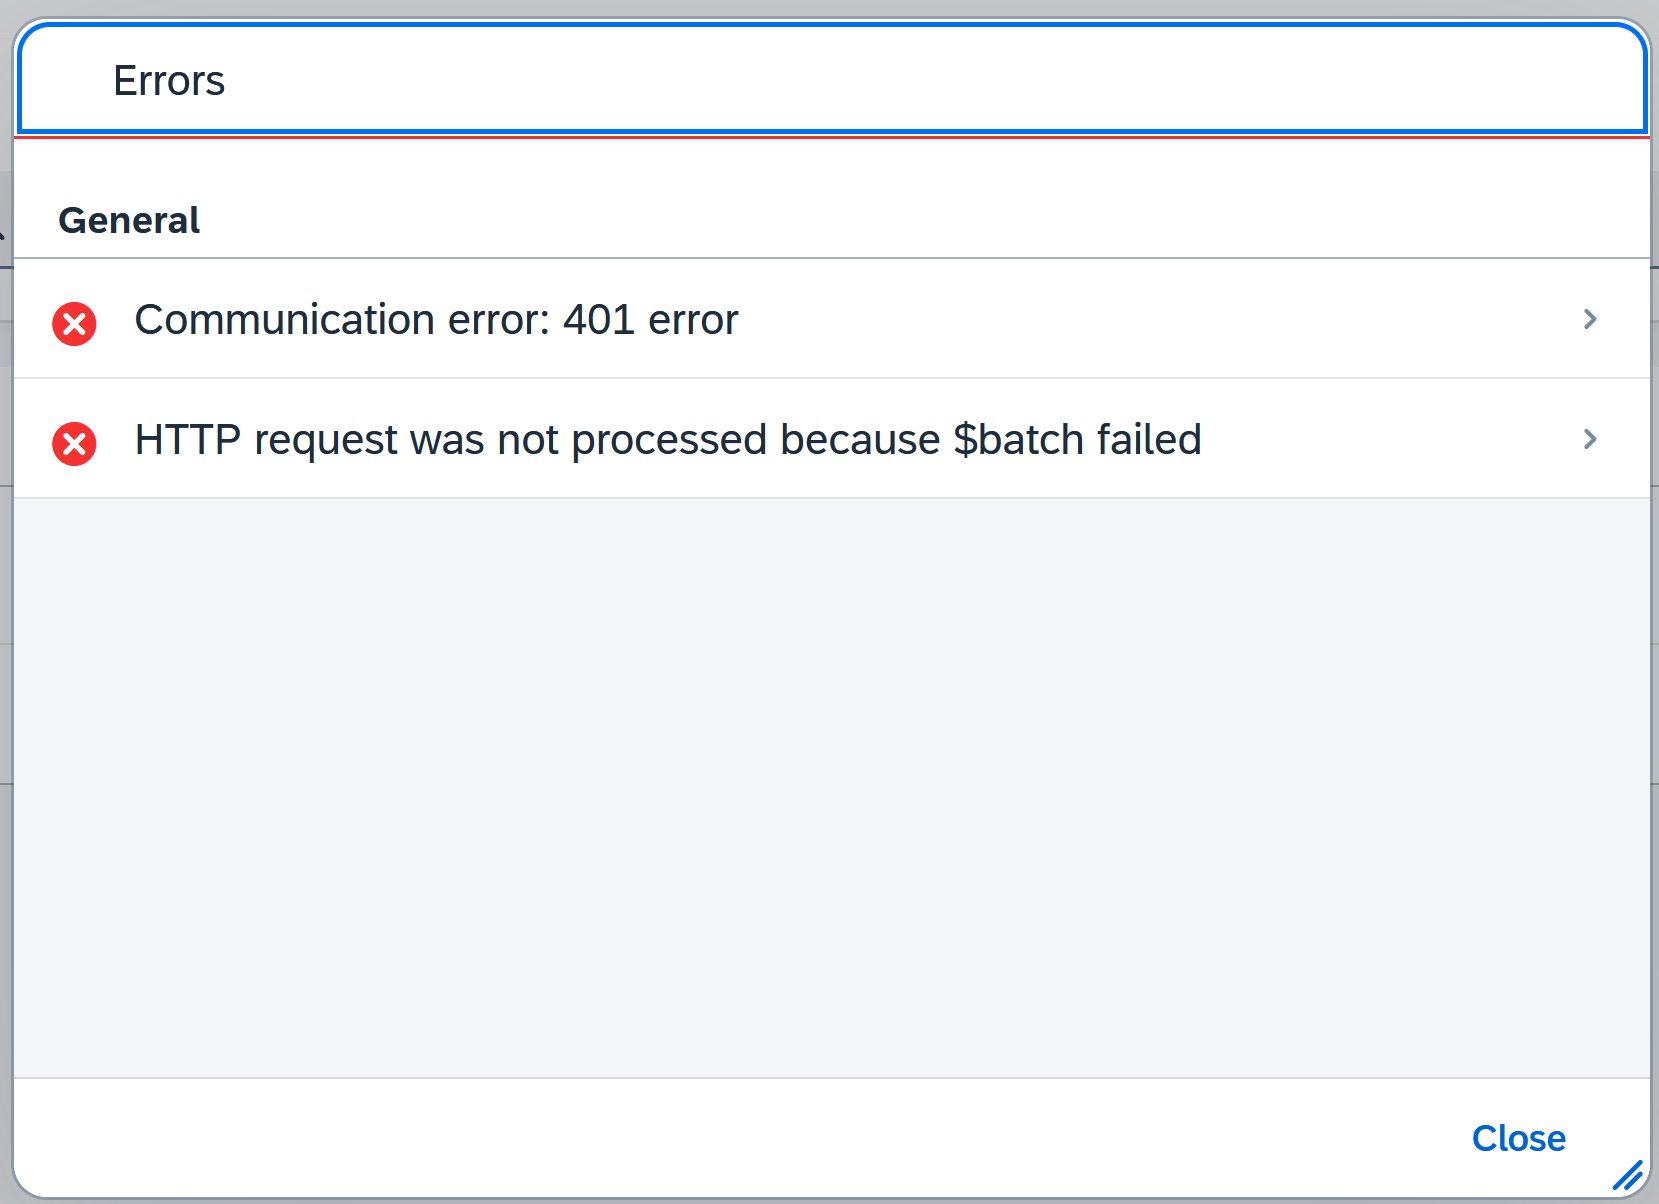
\includegraphics[width=0.5\linewidth]{images/user_doc/overviews/ConnectionError1.png}
	\caption{Illegal Access to Unauthorised Applications - Possible Error}
	\label{fig:IllegalAccesstoUnauthorised Applications}
\end{figure}

\pagebreak

\section{End User}
\label{sec:UdocEndUser}

As a logged in \textbf{End User}, one is granted to access the two applications under the \textbf{My Home} section, namely \textbf{My Packages} (\autoref{subsec:ph}) and \textbf{Package Pickup} (\autoref{subsec:pp}). \textbf{End User} can quick jump to the section by left clicking the "My Home" tab. \textbf{End User} can enter the application by left click the tiles. (\autoref{fig:EndUserApplications})

\begin{figure}[H]
	\centering
	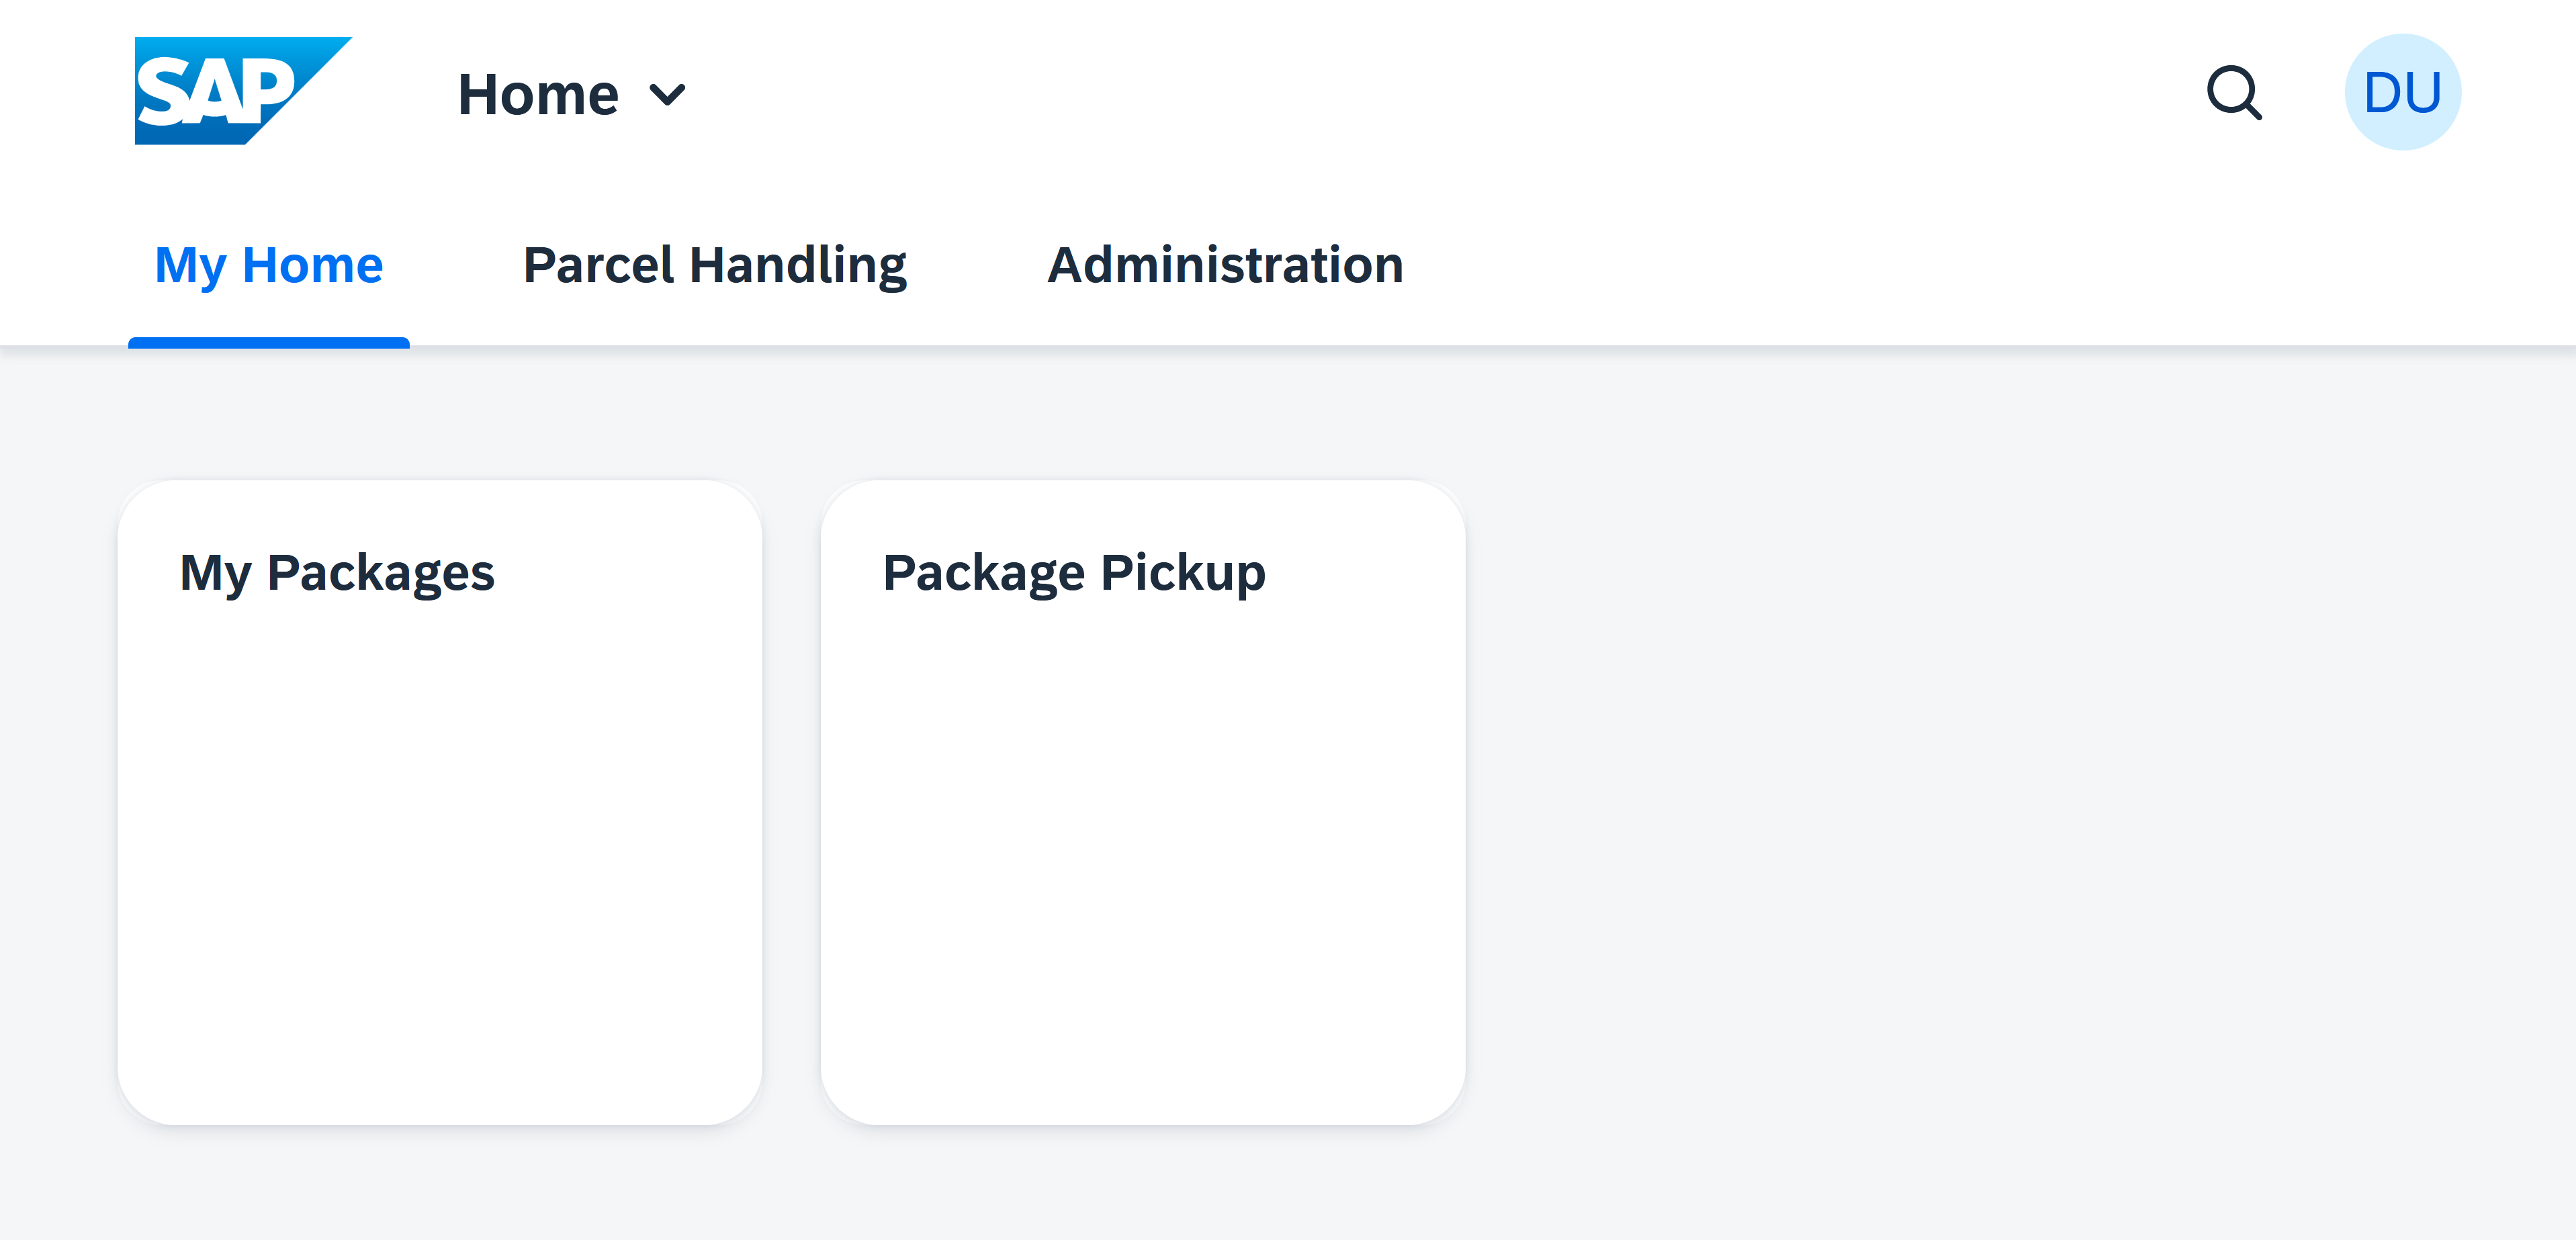
\includegraphics[width=1\linewidth]{images/user_doc/overviews/MyHomeTab.png}
	\caption{End User Applications}
	\label{fig:EndUserApplications}
\end{figure}


% ----------------------- MY PACKAGES ----------------------------
% 
%  ---------------------------------------------------------------

\subsection{My Packages}
\label{subsec:ph}

The \textbf{My Packages} application is here for any \textbf{End User} (See \autoref{sec:UdocEndUser} for all related applications) who would want to check his/her own packages. One can only see one's own packages. 
The summarized main actions the \textbf{End User} can take within the application are listed here:

\begin{compactenum}
	\item Browse the owned package history.
        \begin{compactenum}
        	\item Filter possibility.
            \item List report for packages.
        \end{compactenum}
\end{compactenum}

\subsubsection{Home Screen - Overview}
As an \textbf{End User}, after clicking at the application tile, is redirected to the "Home Screen" (\autoref{fig:HistoryHome}), which is the main and only screen of this application. The upper part displays the search bar and the possible filters. While the lower part displays the list of packages. The information provides for each packages are: \textbf{Type} (the type of the package, existing types are newspaper, letter and normal), \textbf{Status} (the status of the package, existing status are new, confirmed and picked up), \textbf{Delivery Company} (the delivery company of the package), \textbf{Delivery Time} (the confirmation time of the package, if applicable), \textbf{Pickup Time} (the picked up time of the package, if applicable).

\begin{figure}[H]
	\centering
	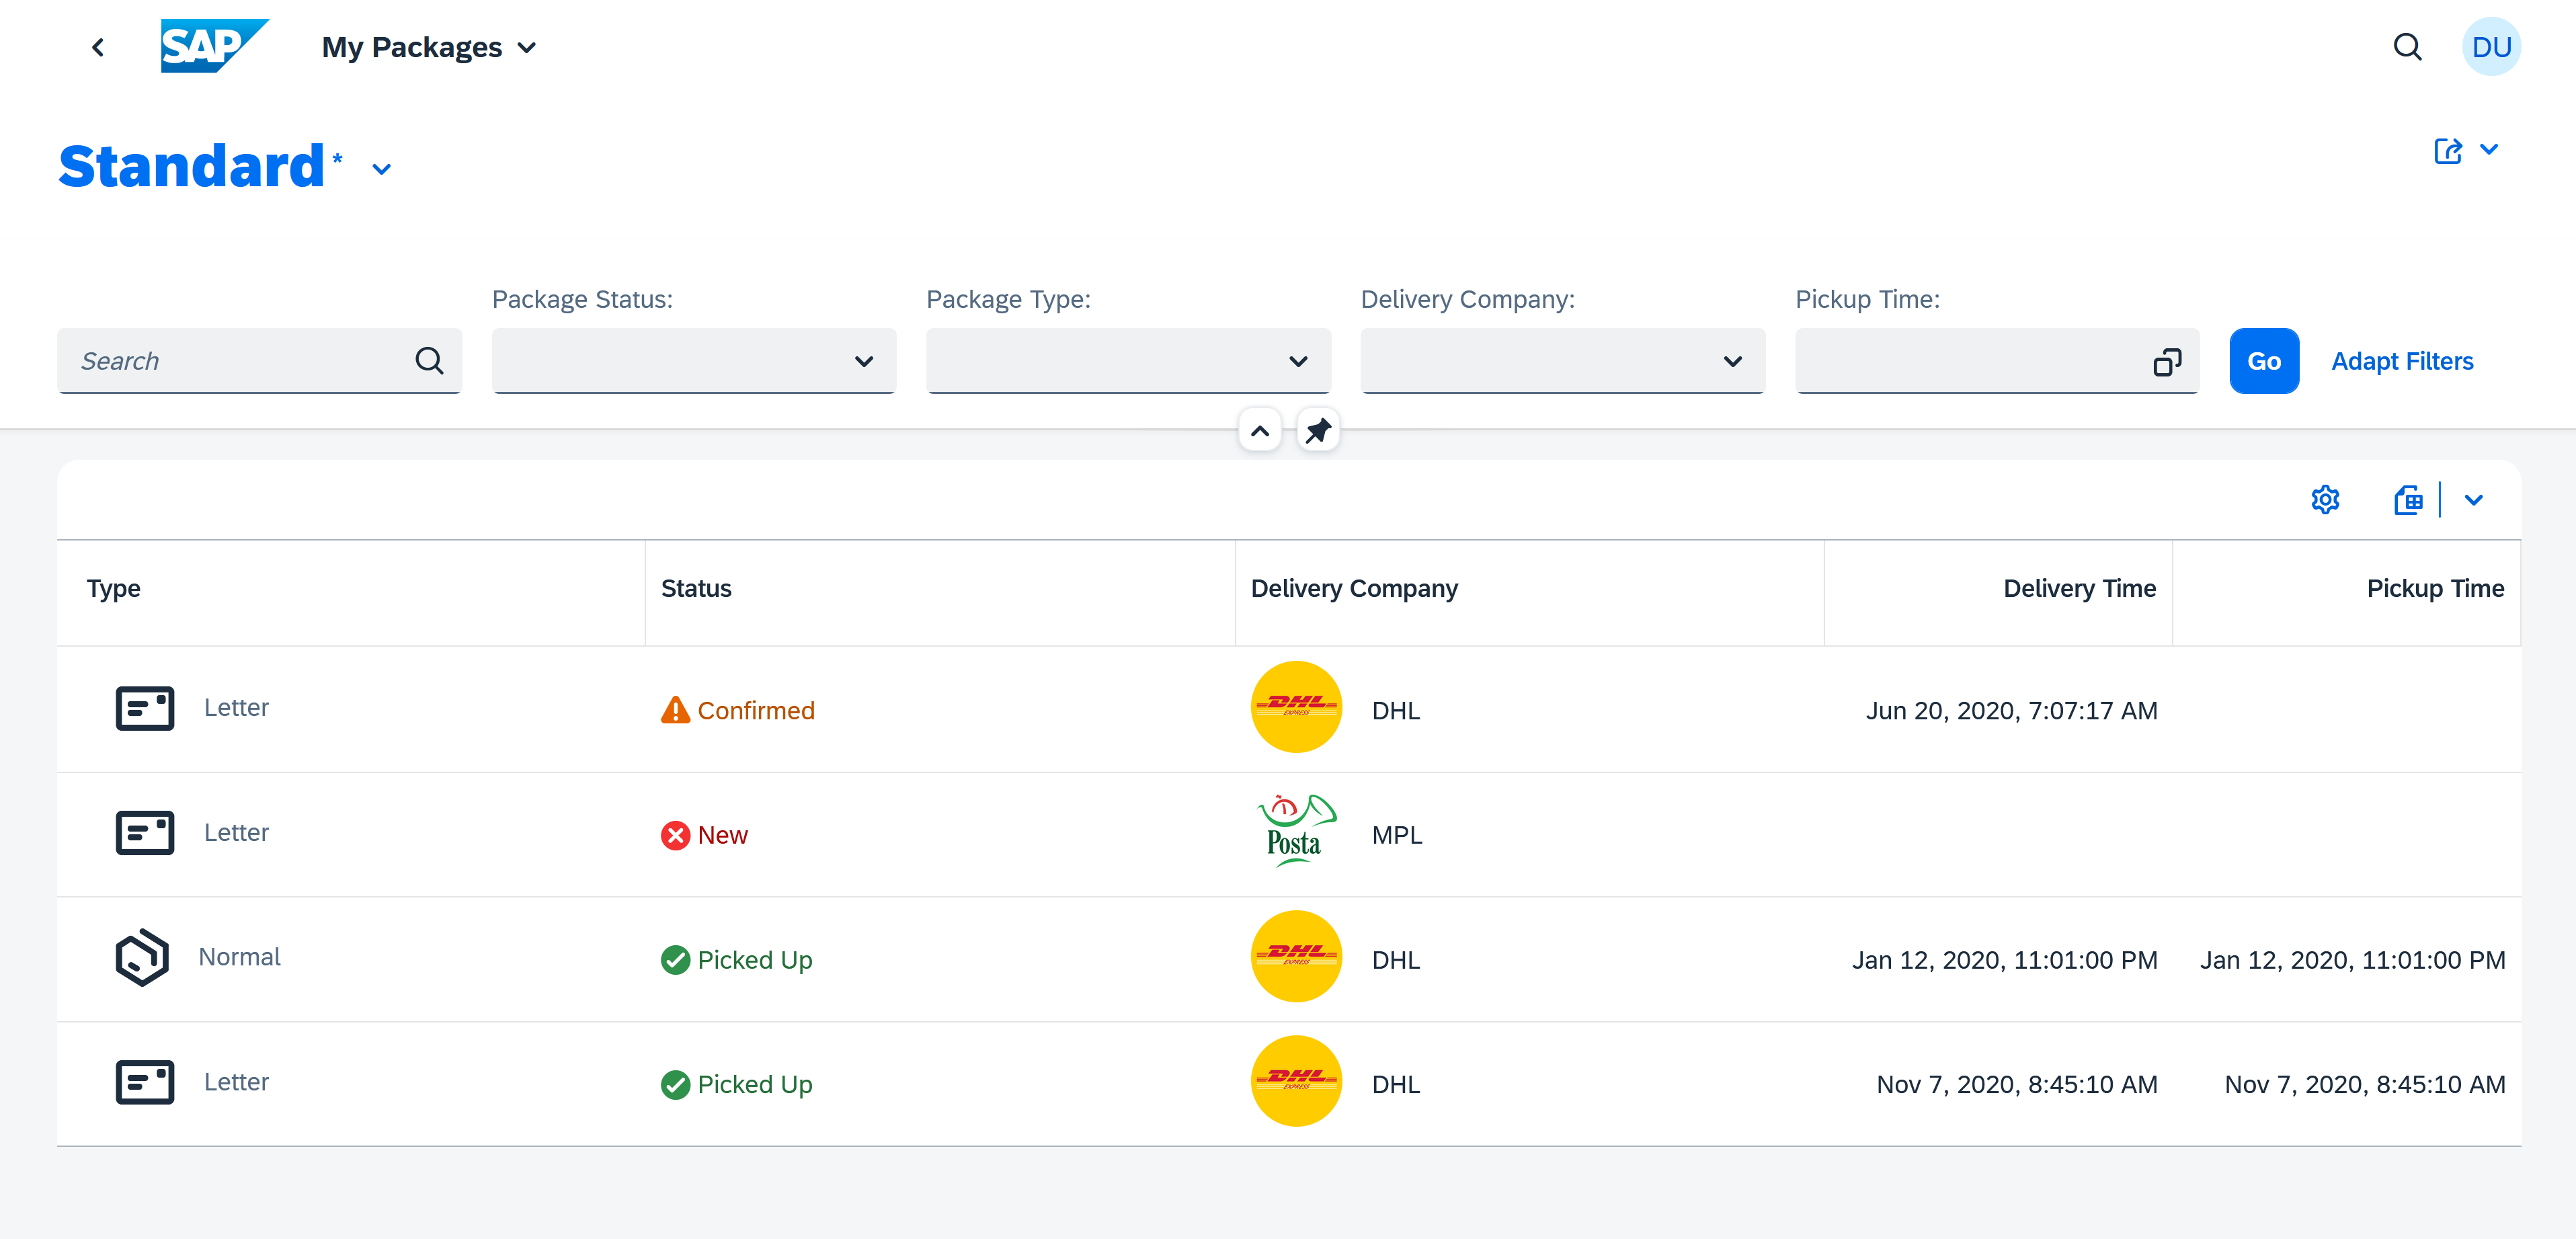
\includegraphics[width=1\linewidth]{images/user_doc/myPack/overview.png}
	\caption{History Home Screen - Overview}
	\label{fig:HistoryHome}
\end{figure}

\subsubsection{Home Screen - Filter Usage}
One can type in free text of any possible content of the column in the "Search Bar" (\autoref{fig:mpSearchBar}). The free text supports in-completed keywords and is case insensitive. 
One can use the default filters (\textbf{Status} (drop down), \textbf{Type} (drop down), \textbf{Delivery Company} (drop down) and \textbf{Pickup Time} (time entry) (\autoref{fig:MPDF}). For drop down filters, one can click at the small drop down arrow and select zero to many options. For time entry, one shall click at the "double box" (filter help) on the right of the filter box. This will pops up a dialog, at where one can select the desired filtering option and enter the time with the clock uitility (\autoref{fig:PHAjustTimeFilters}). One can also access to more filters (\textbf{Delivery Time} (time entry) by clicking at "Adapt Filters". (\autoref{fig:mpMOreFilterAdaption}) While adjusting the filtering values, the list view is temporarily locked. After adjusting the filtering values, run the filter by clicking the "Go" Button. (\autoref{fig:PHAjustFilters-2})

\begin{figure}[H]
	\centering
	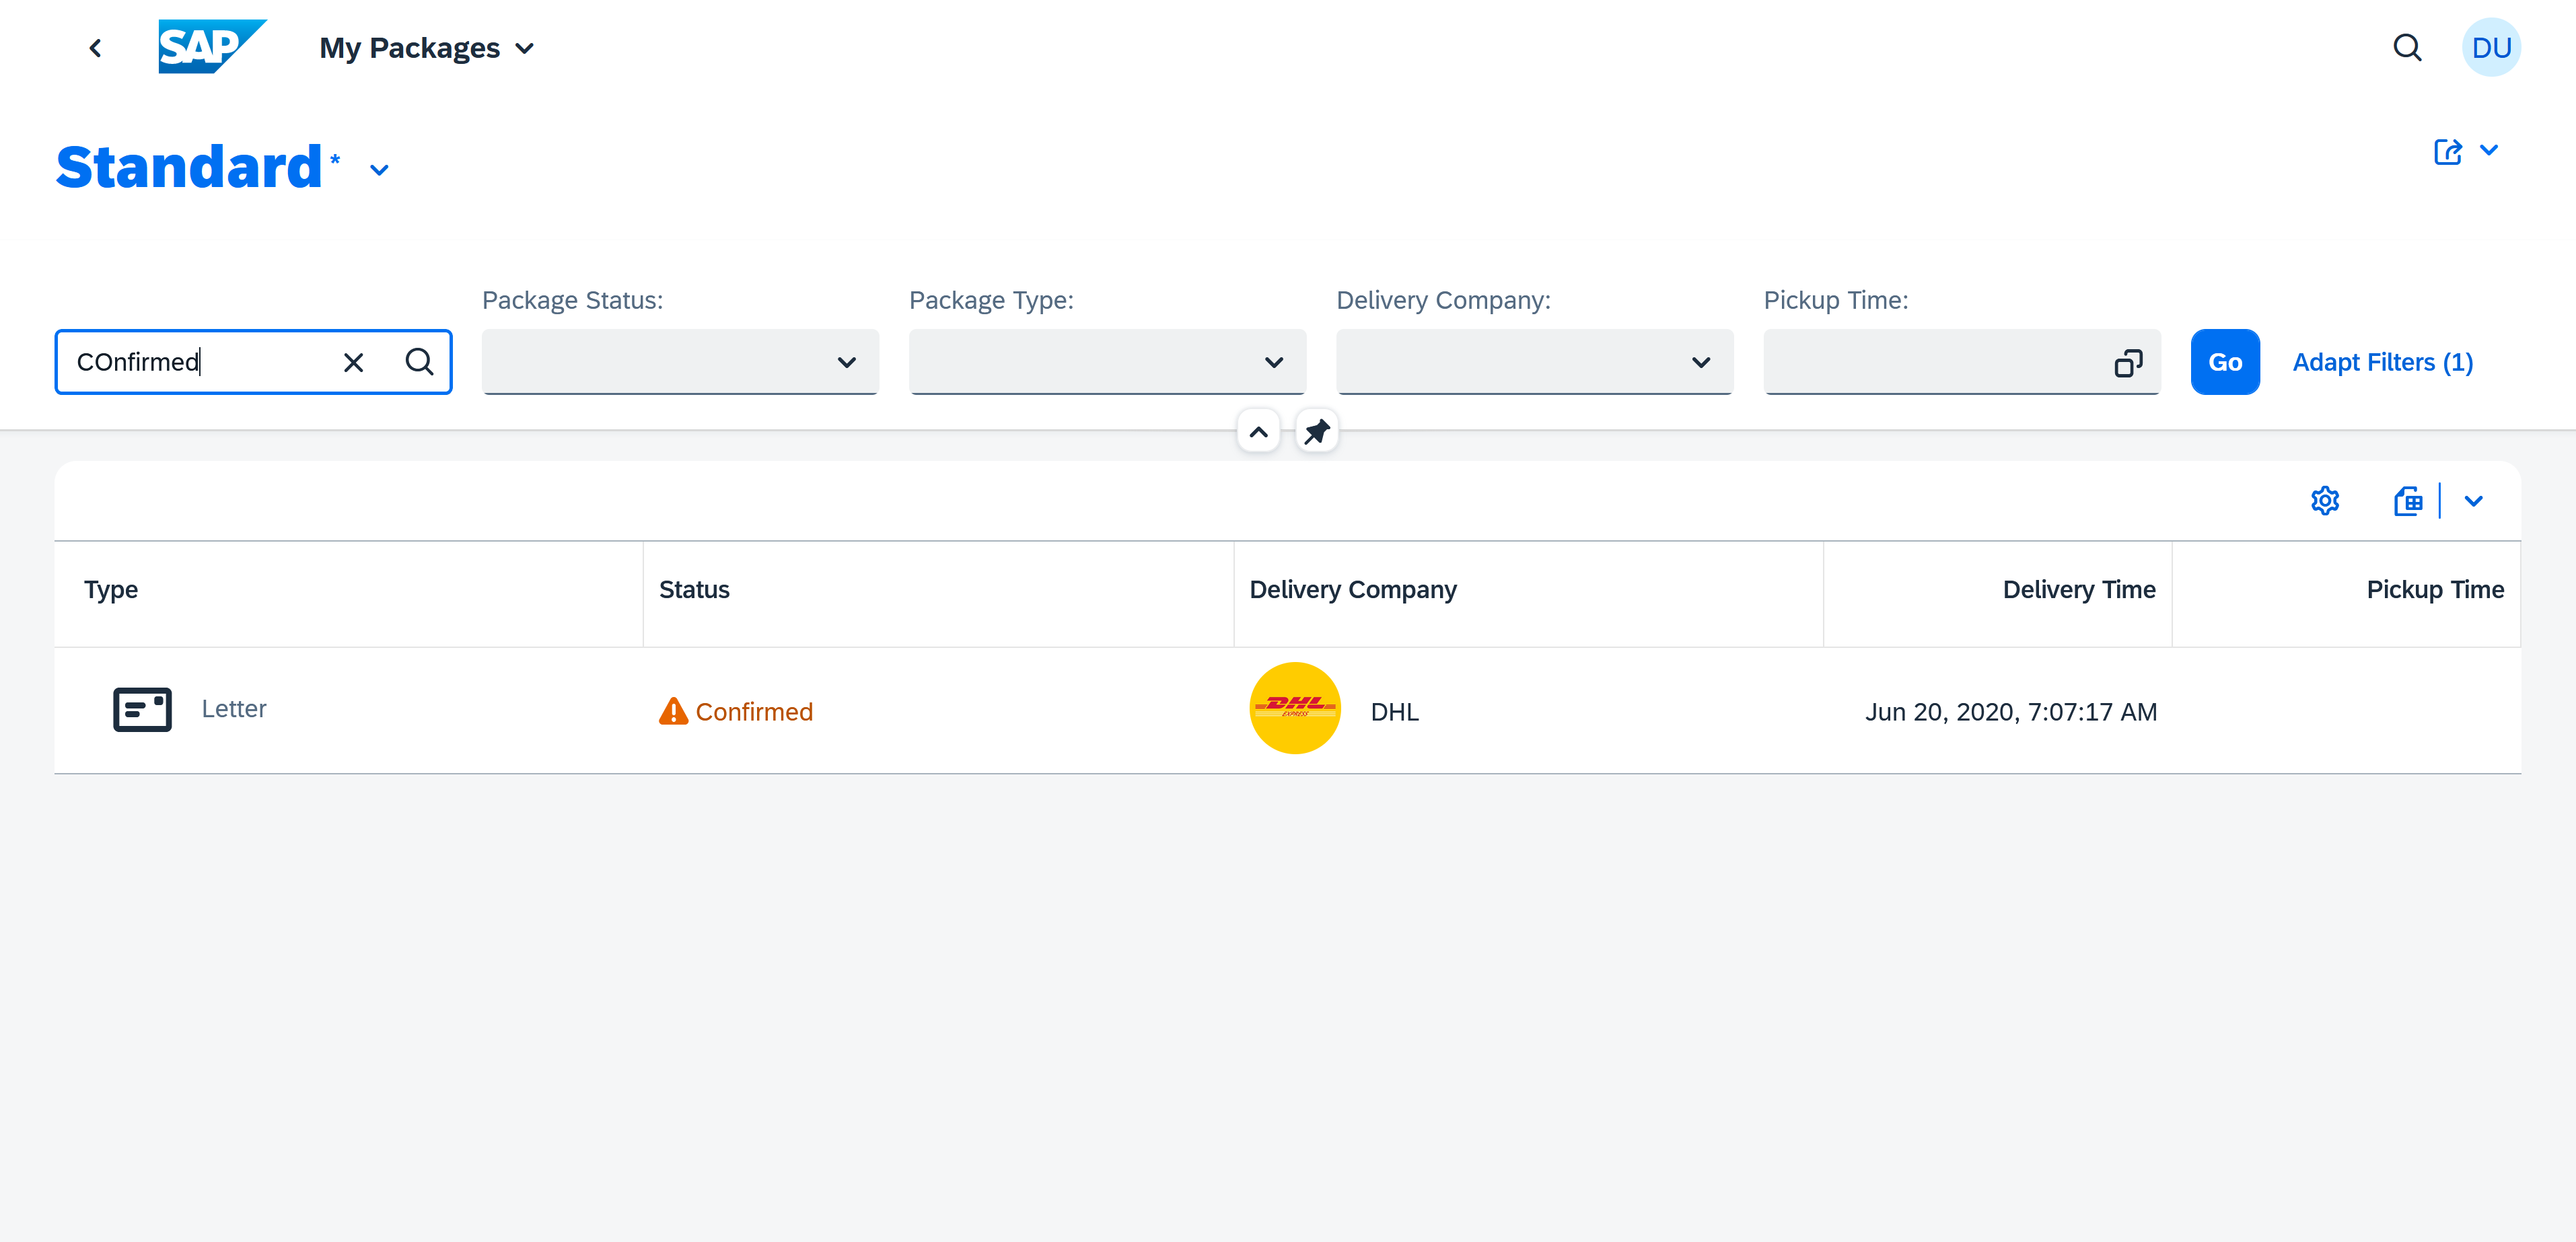
\includegraphics[width=1\linewidth]{images/user_doc/myPack/searchbar.png}
	\caption{My Package Home Screen - Search Bar}
	\label{fig:mpSearchBar}
\end{figure}


\begin{figure}[H]
	\centering
	\subcaptionbox{Status Filter}{
		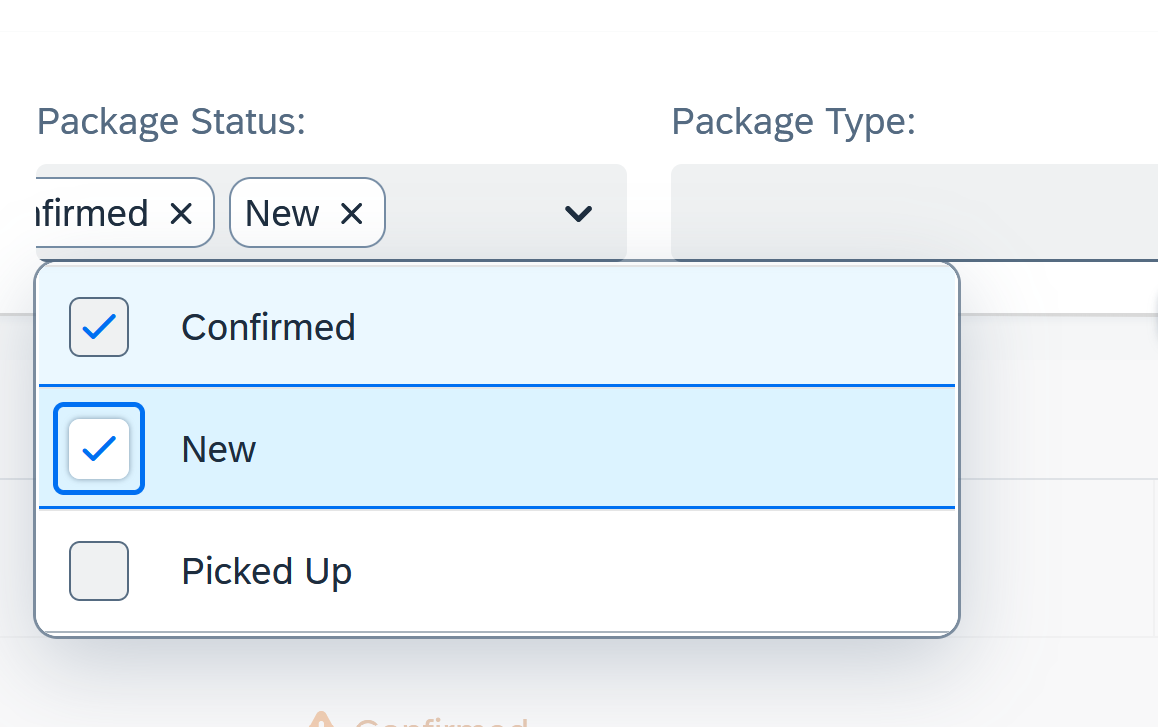
\includegraphics[width=0.45\linewidth]{images/user_doc/myPack/statusFIlter.png}}
	\hspace{5pt}
	\subcaptionbox{Type Filter}{
		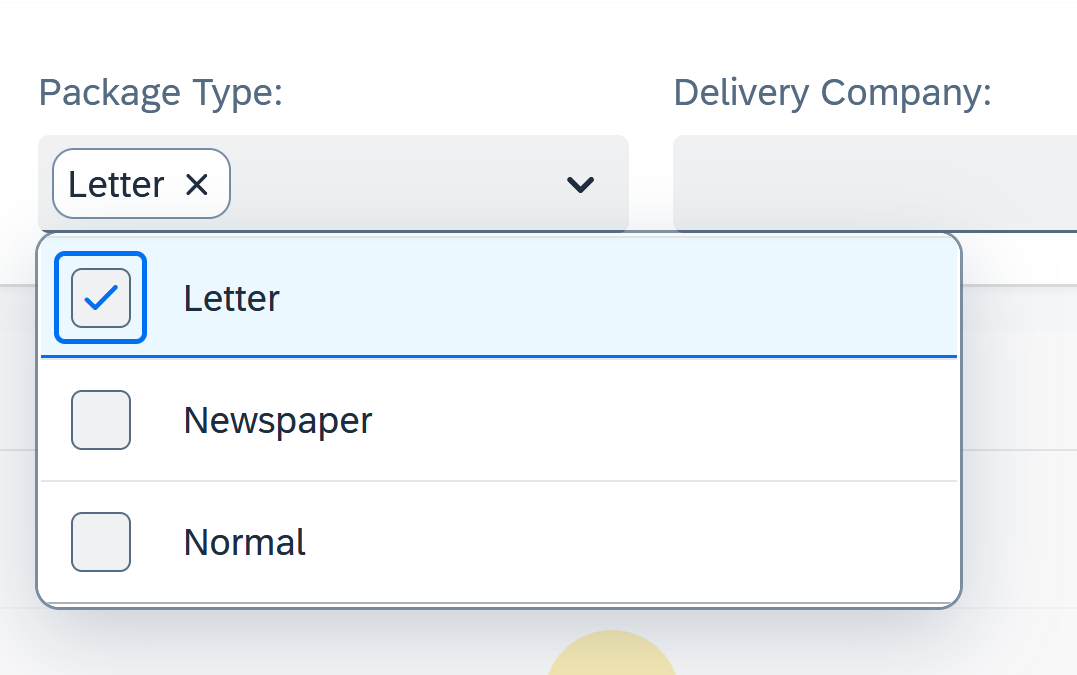
\includegraphics[width=0.45\linewidth]{images/user_doc/myPack/typeFIlter.png}}

    \subcaptionbox{Company Filter}{
		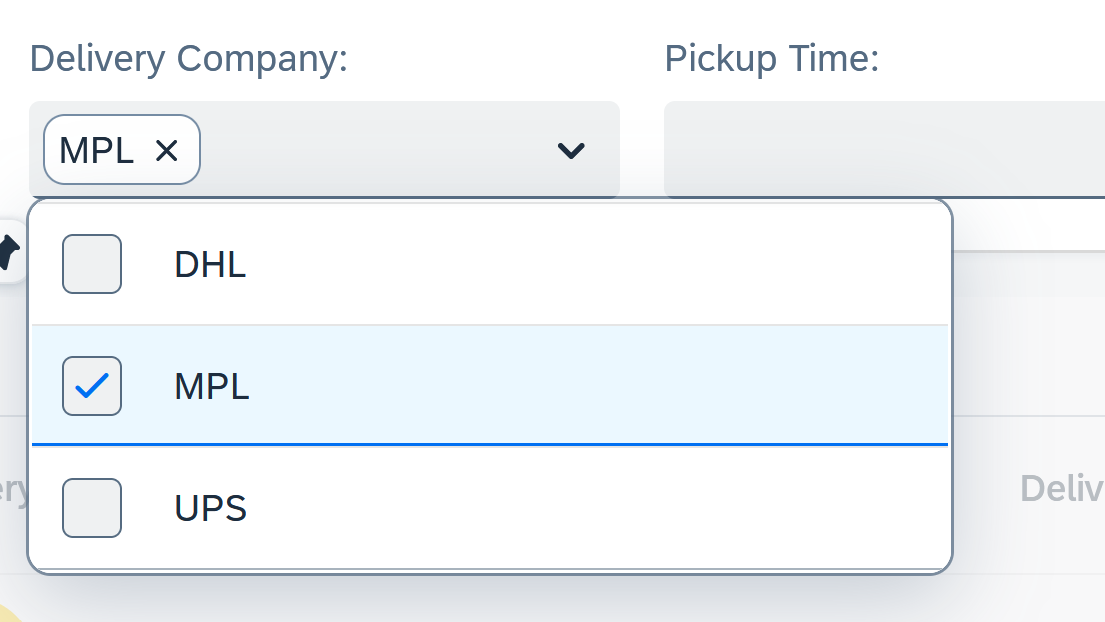
\includegraphics[width=0.45\linewidth]{images/user_doc/myPack/companyFilter.png}}
	\hspace{5pt}
	\subcaptionbox{Time Filter}{
		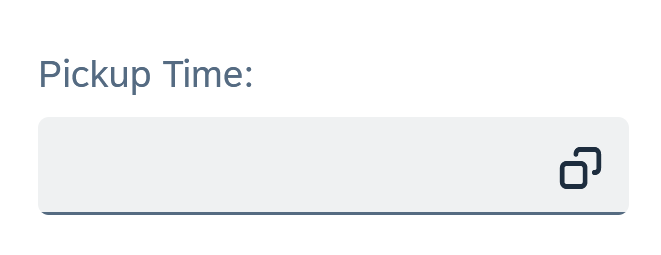
\includegraphics[width=0.45\linewidth]{images/user_doc/myPack/timeFilter.png}}
	\caption{My Package Home Screen - Default Filters}
	\label{fig:MPDF}
\end{figure}

\begin{figure}[H]
		\centering
	\subcaptionbox{Time Filter Options Selections}{
		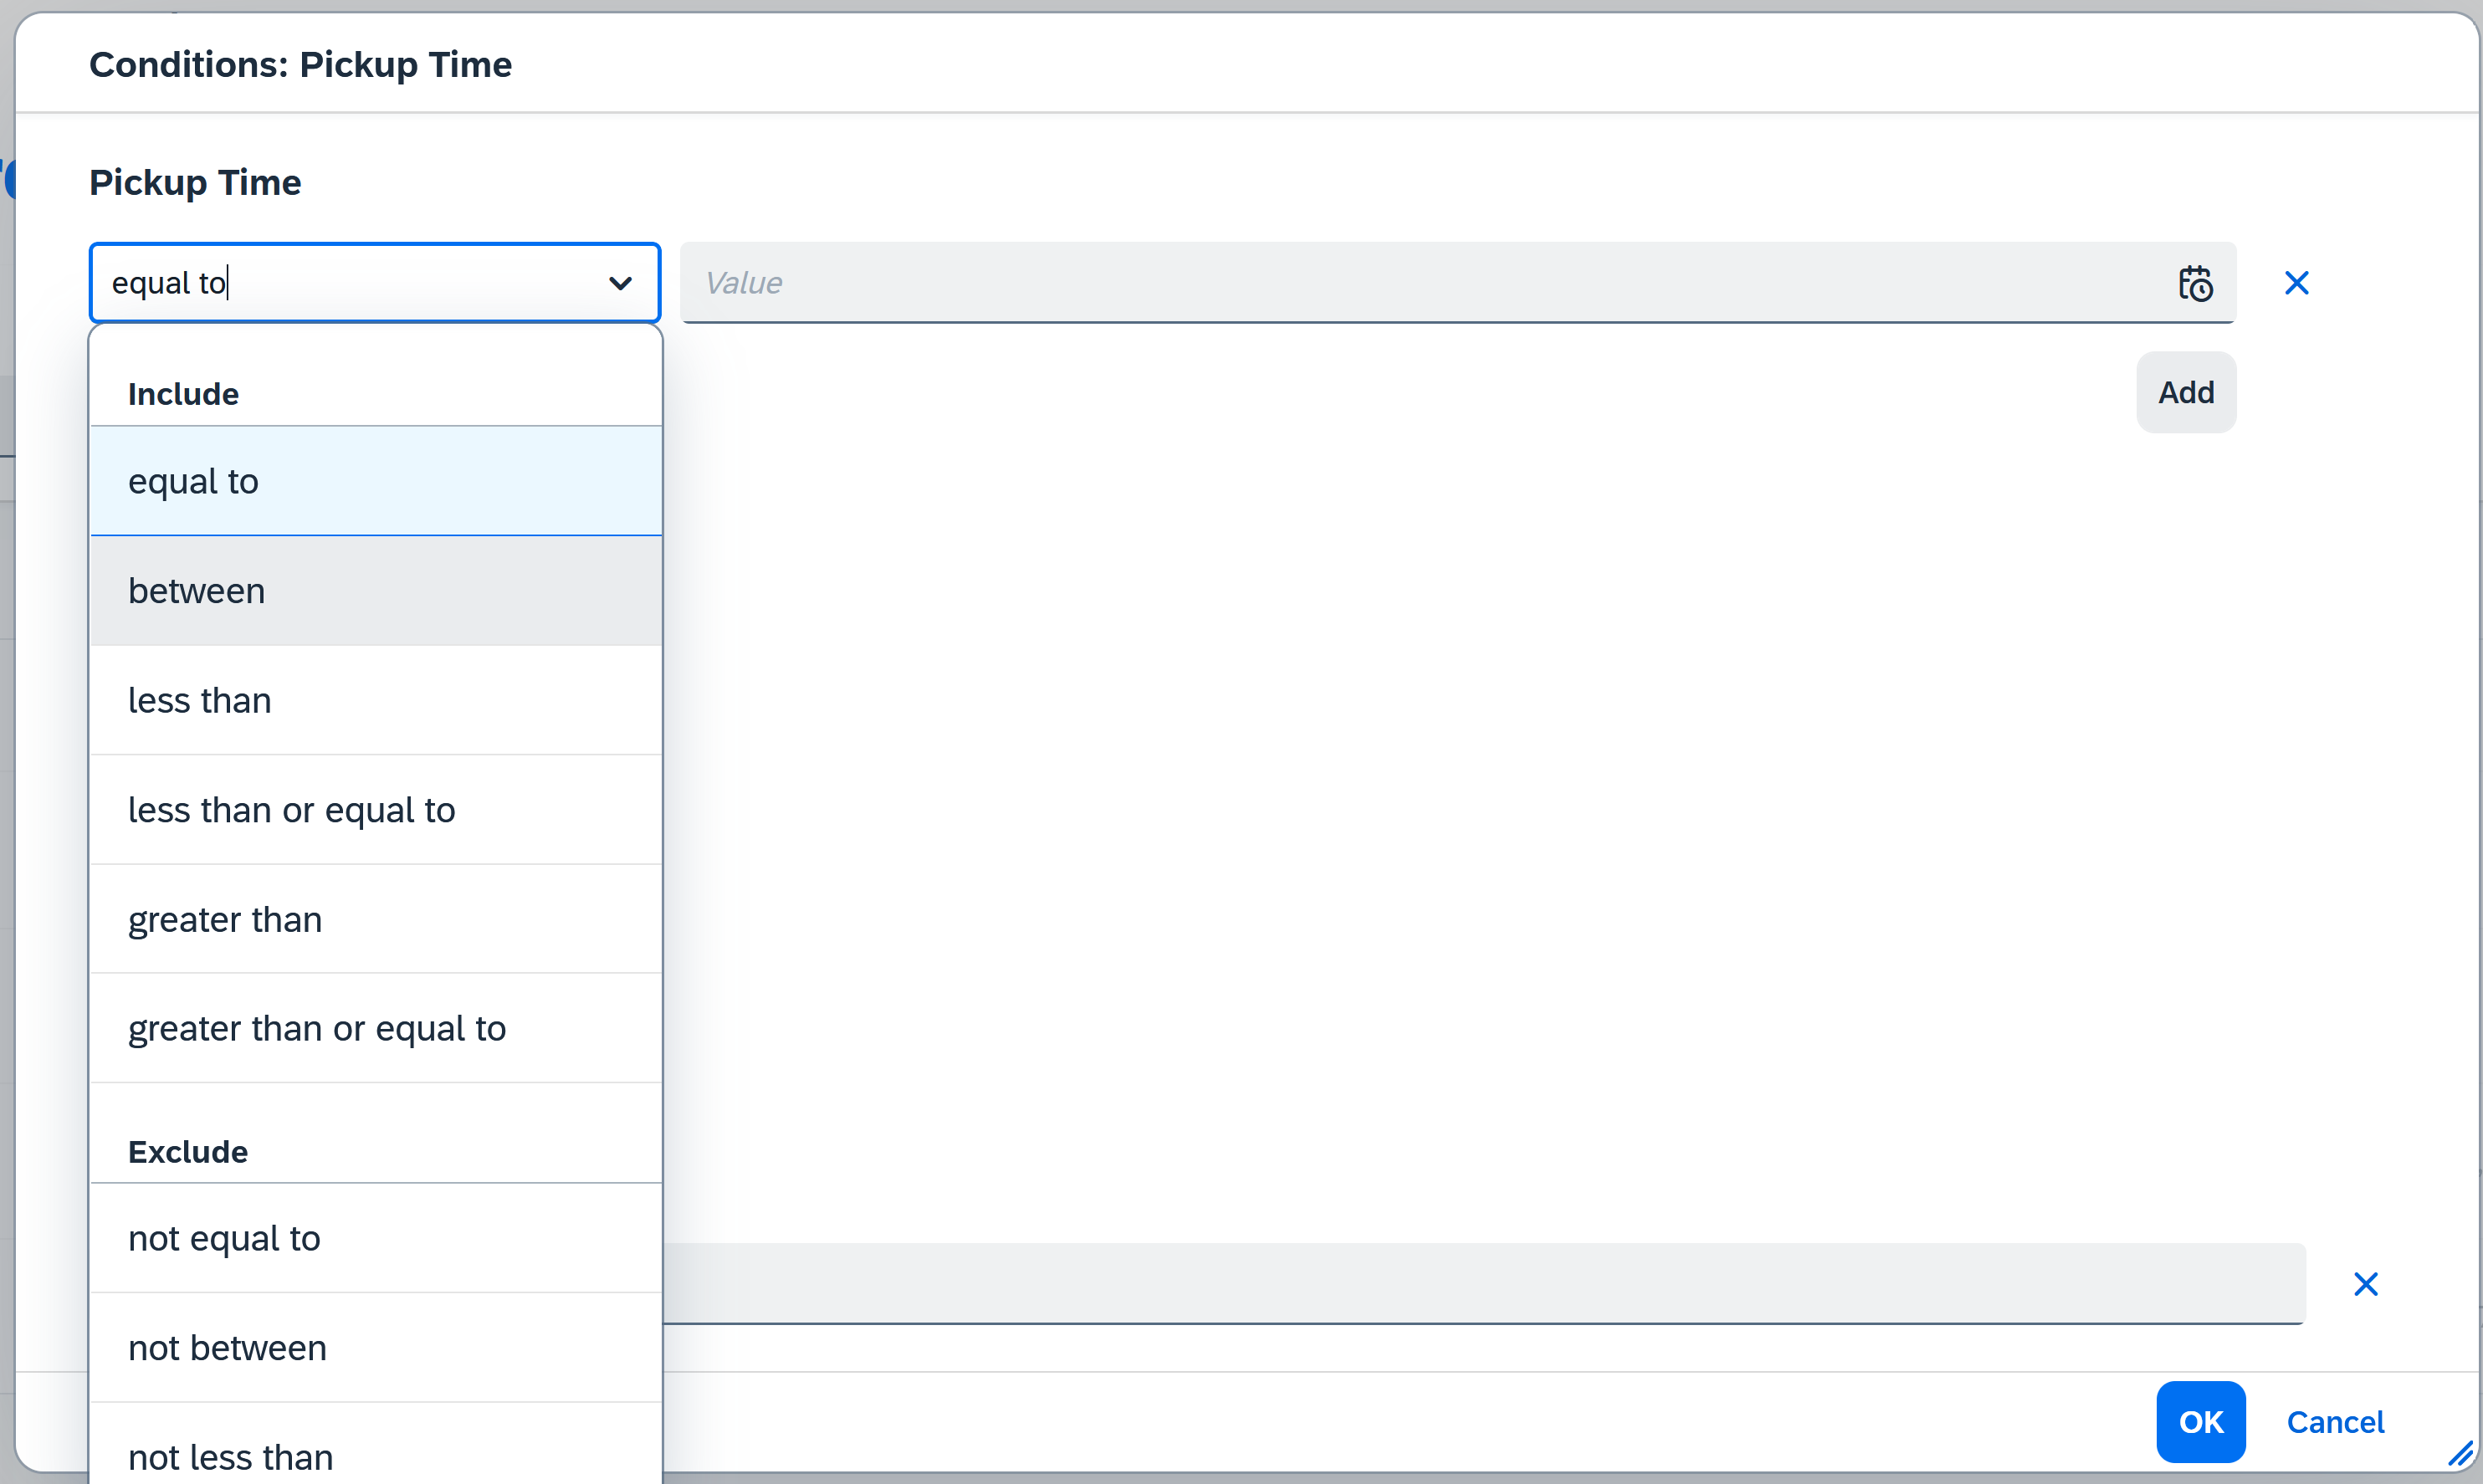
\includegraphics[width=0.45\linewidth]{images/user_doc/myPack/timeFilter_Usage1.png}}
	\hspace{5pt}
	\subcaptionbox{Time Entry}{
		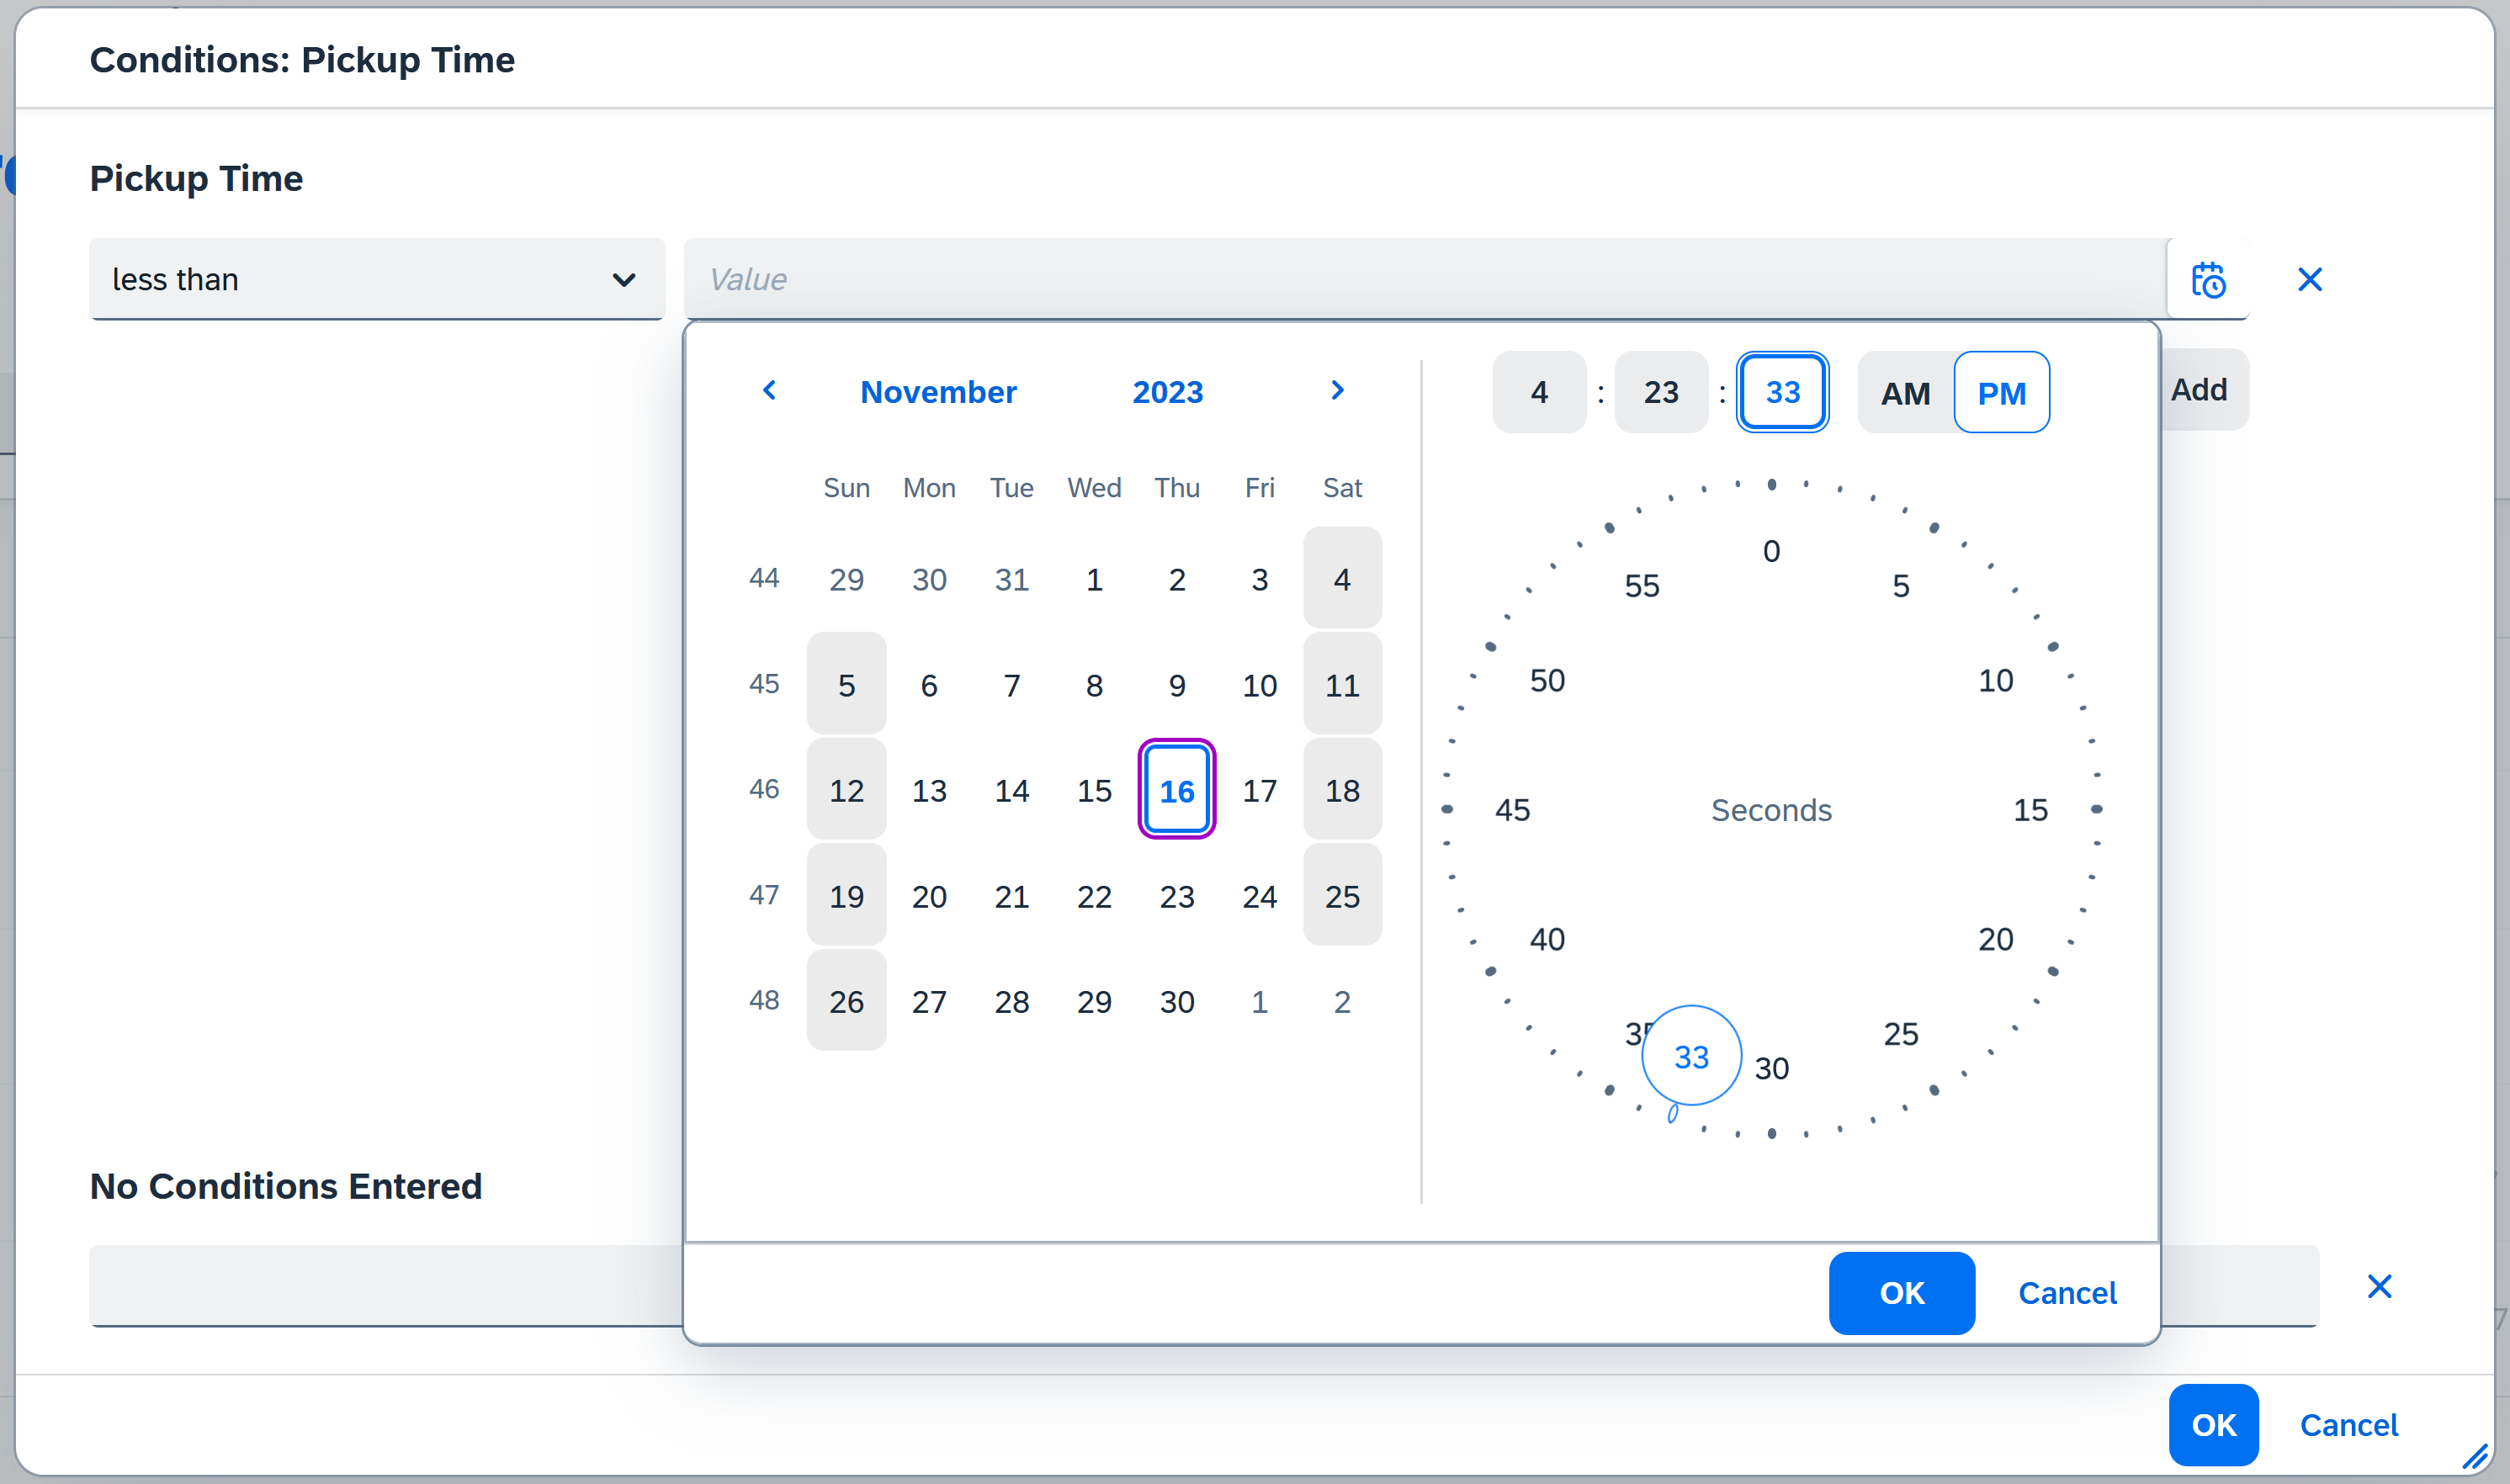
\includegraphics[width=0.45\linewidth]{images/user_doc/myPack/timeFilter-Usage2.png}}
    \caption{Time Filter Dialog - Adjust Filters}
    \label{fig:PHAjustTimeFilters}
\end{figure}


\begin{figure}[H]
		\centering
	\subcaptionbox{While Adjusting the Filter}{
		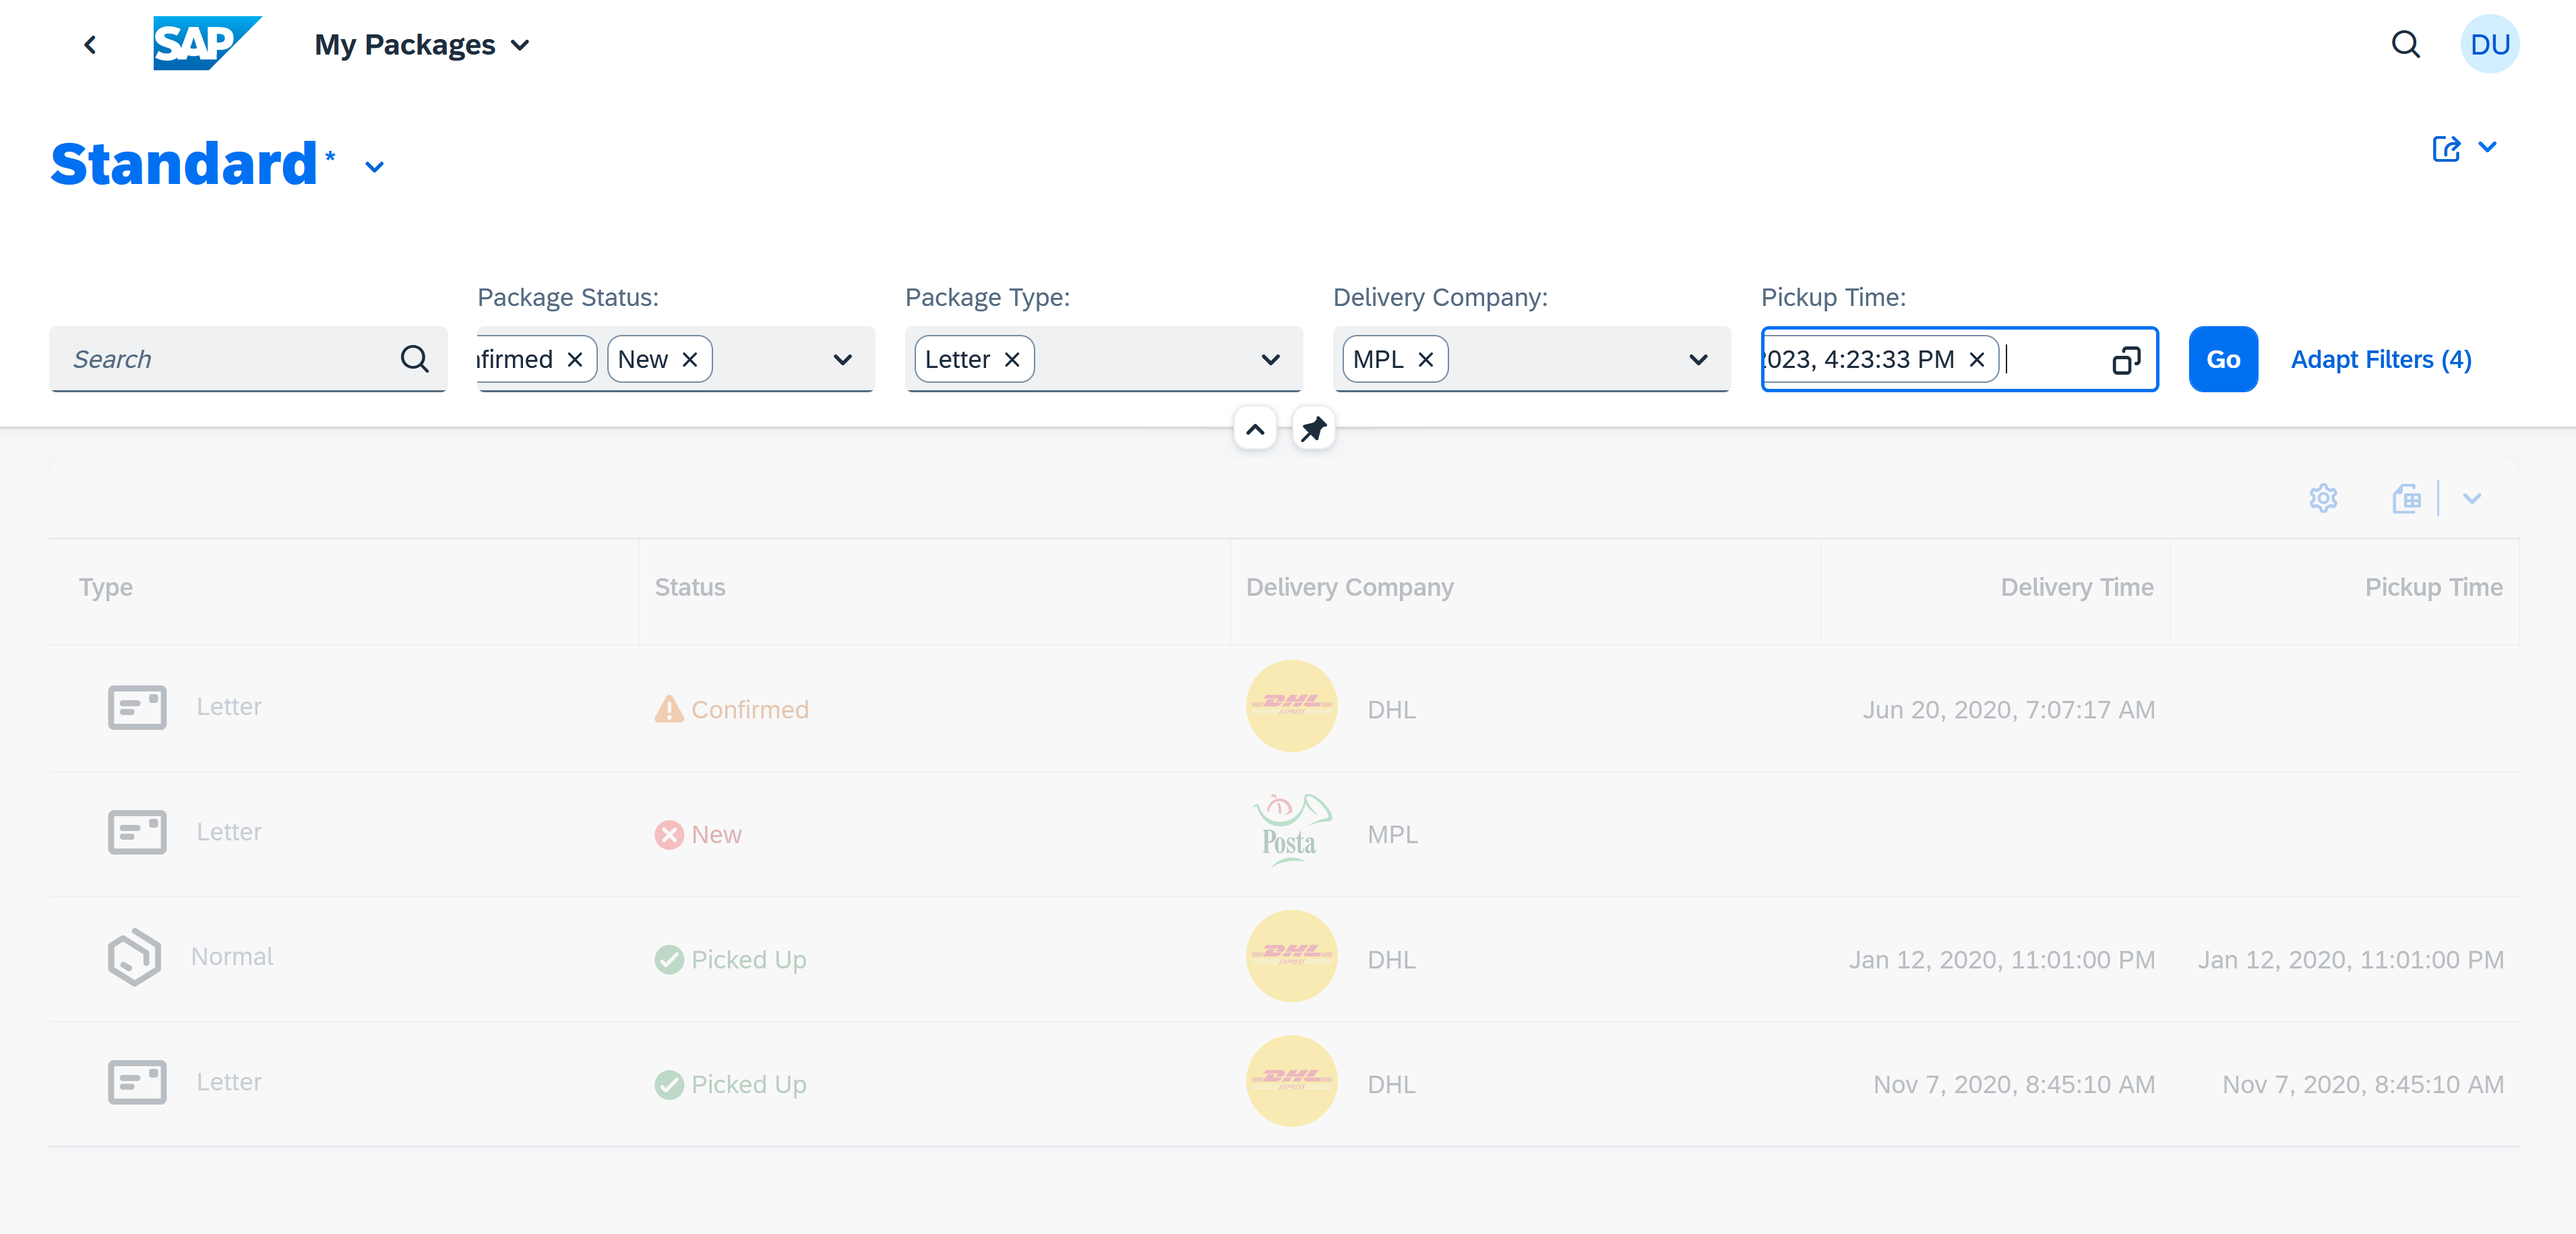
\includegraphics[width=0.45\linewidth]{images/user_doc/myPack/filterAdaptionScreen.png}}
	\hspace{5pt}
	\subcaptionbox{Clicked "Go"}{
		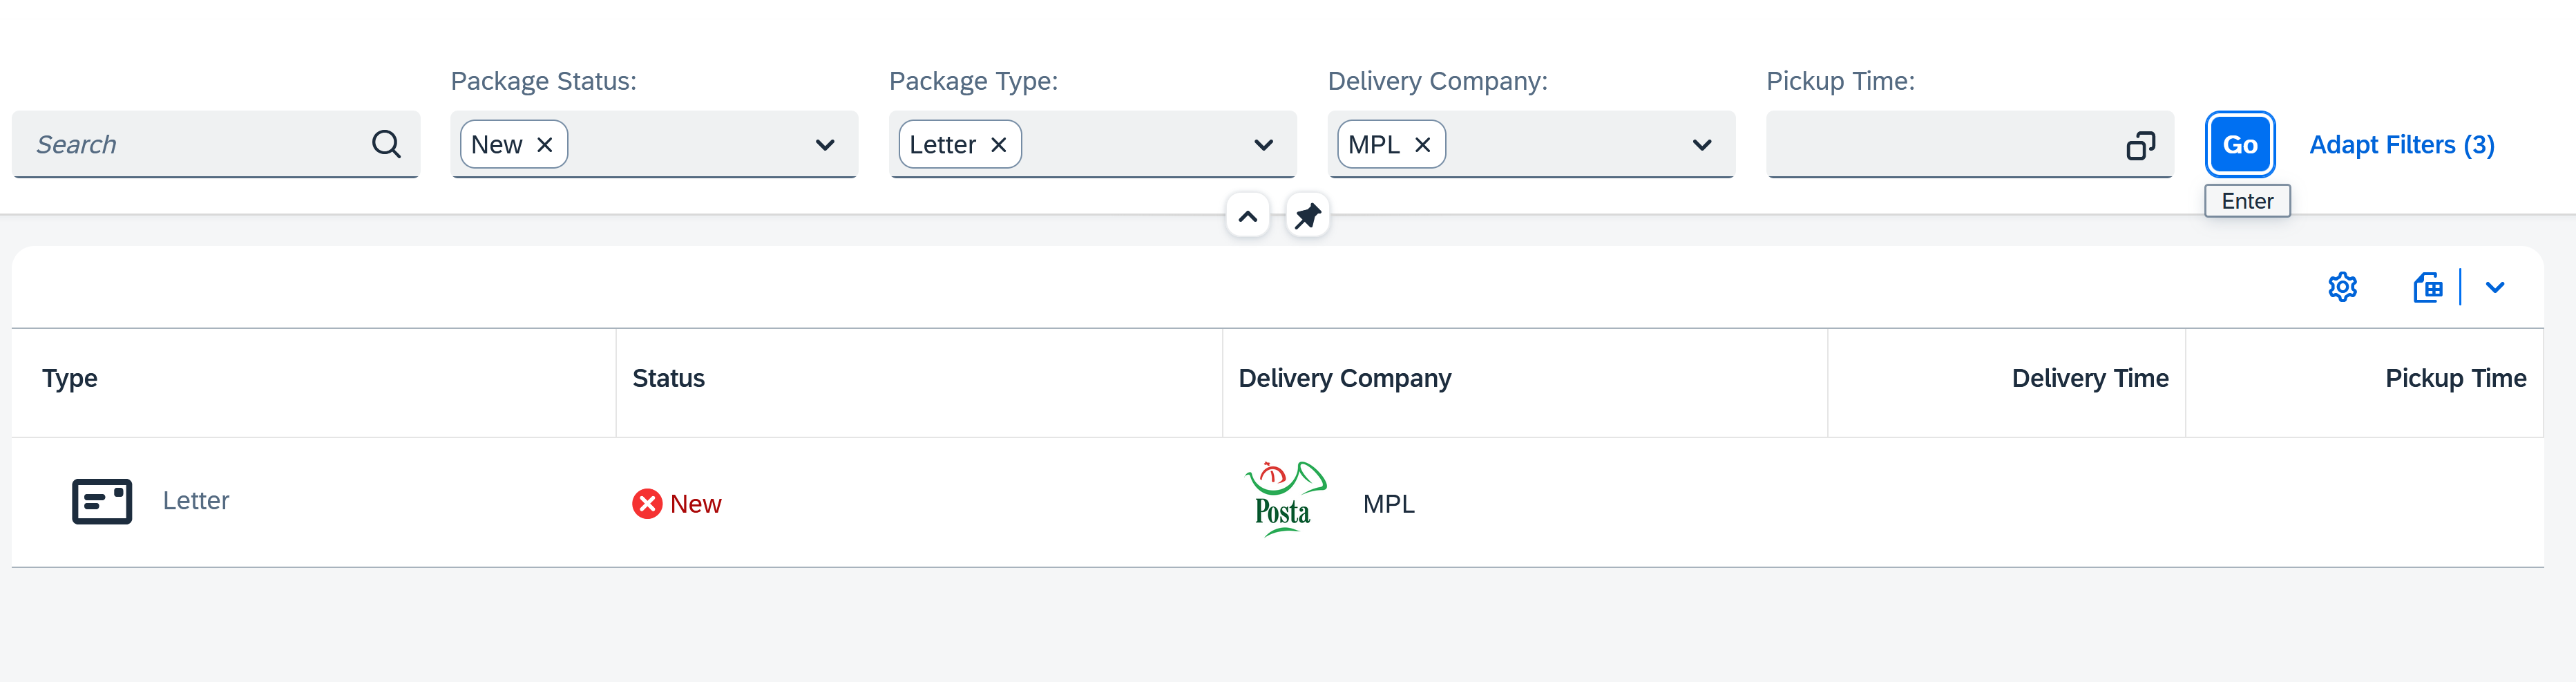
\includegraphics[width=0.45\linewidth]{images/user_doc/myPack/FilterDoneScreen.png}}
    \caption{My Package Home Screen - Adjust Filters}
    \label{fig:PHAjustFilters-2}
\end{figure}

\begin{figure}[H]
	\centering
	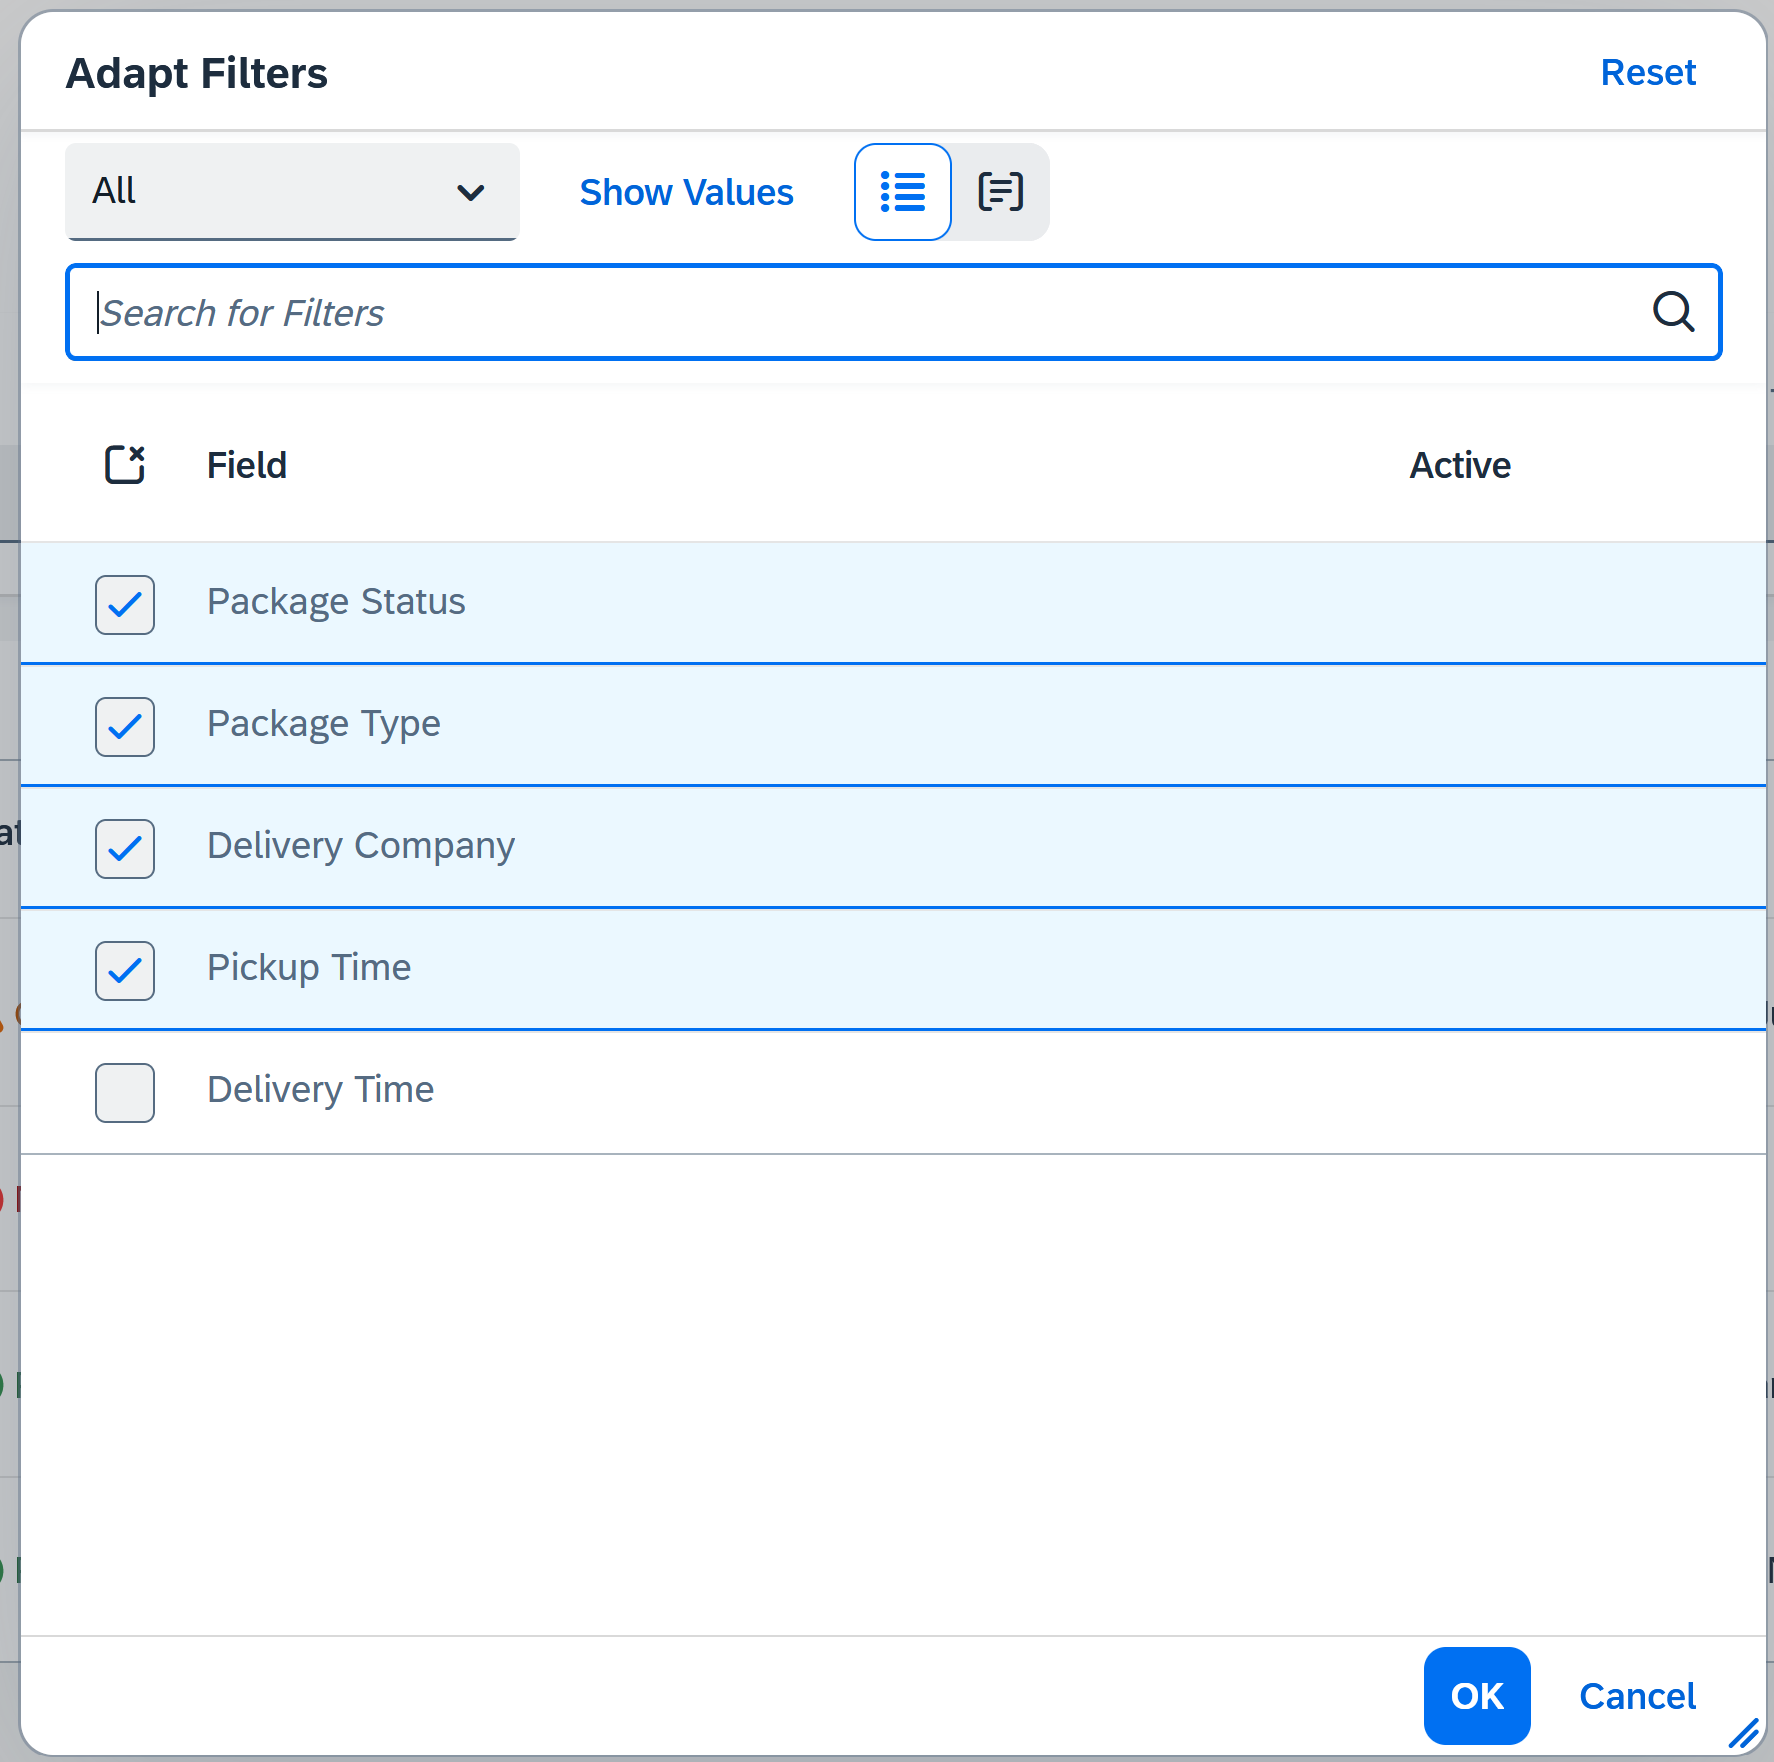
\includegraphics[height=200pt]{images/user_doc/myPack/MoreFIlterOption.png}
	\caption{My Package Filter Adaption Dialog - More Filters}
	\label{fig:mpMOreFilterAdaption}
\end{figure}
% ----------------------- Package Pickup ----------------------------
% 
%  ---------------------------------------------------------------

\subsection{Package Pickup}
\label{subsec:pp}

The \textbf{Package Pickup} application is used to pick up any confirmed parcels (registered at the reception and confirmed with a storage slot) of the logged in user. One can only see one's own confirmed packages. 
The summarized main actions the \textbf{End User} (See \autoref{sec:UdocEndUser} for all related applications) can take within the application are listed here:

\begin{compactenum}
	\item Browse the owned packages that can be picked up.
    \item Pickup the listed owned packages.
\end{compactenum}

\bigskip
\textbf{Hint}: The application supports only from mobile devices. In case an employee is unable to access his or her mobile at the moment of pickup, he or she shall ask the receptionist to pickup the package for him or her.


\subsubsection{Home Screen - Selection}
As an \textbf{End User}, after clicking at the application tile, is redirected to the "Home Screen". If there exists at least one package to pickup, the home screen shows the list of packages. 
The list items lists \textbf{the type with icon, the delivery company, the registration time and the location} of the packages. 
If no package exists to pickup, it shows only the no package info. 
The package list title shows the total number of packages that can be pickup.
In case there are existing packages, one can select one or multiple packages from the list to pickup. 
In case there are existing packages, one can tick/untick the "Toggle All" selection box to select or deselect the package all at once. 
(\autoref{fig:PickupHomeScreen-1}, \autoref{fig:PickupHomeScreen-2})

\begin{figure}[H]
	\centering
	\subcaptionbox{Home Screen with Packages}{
		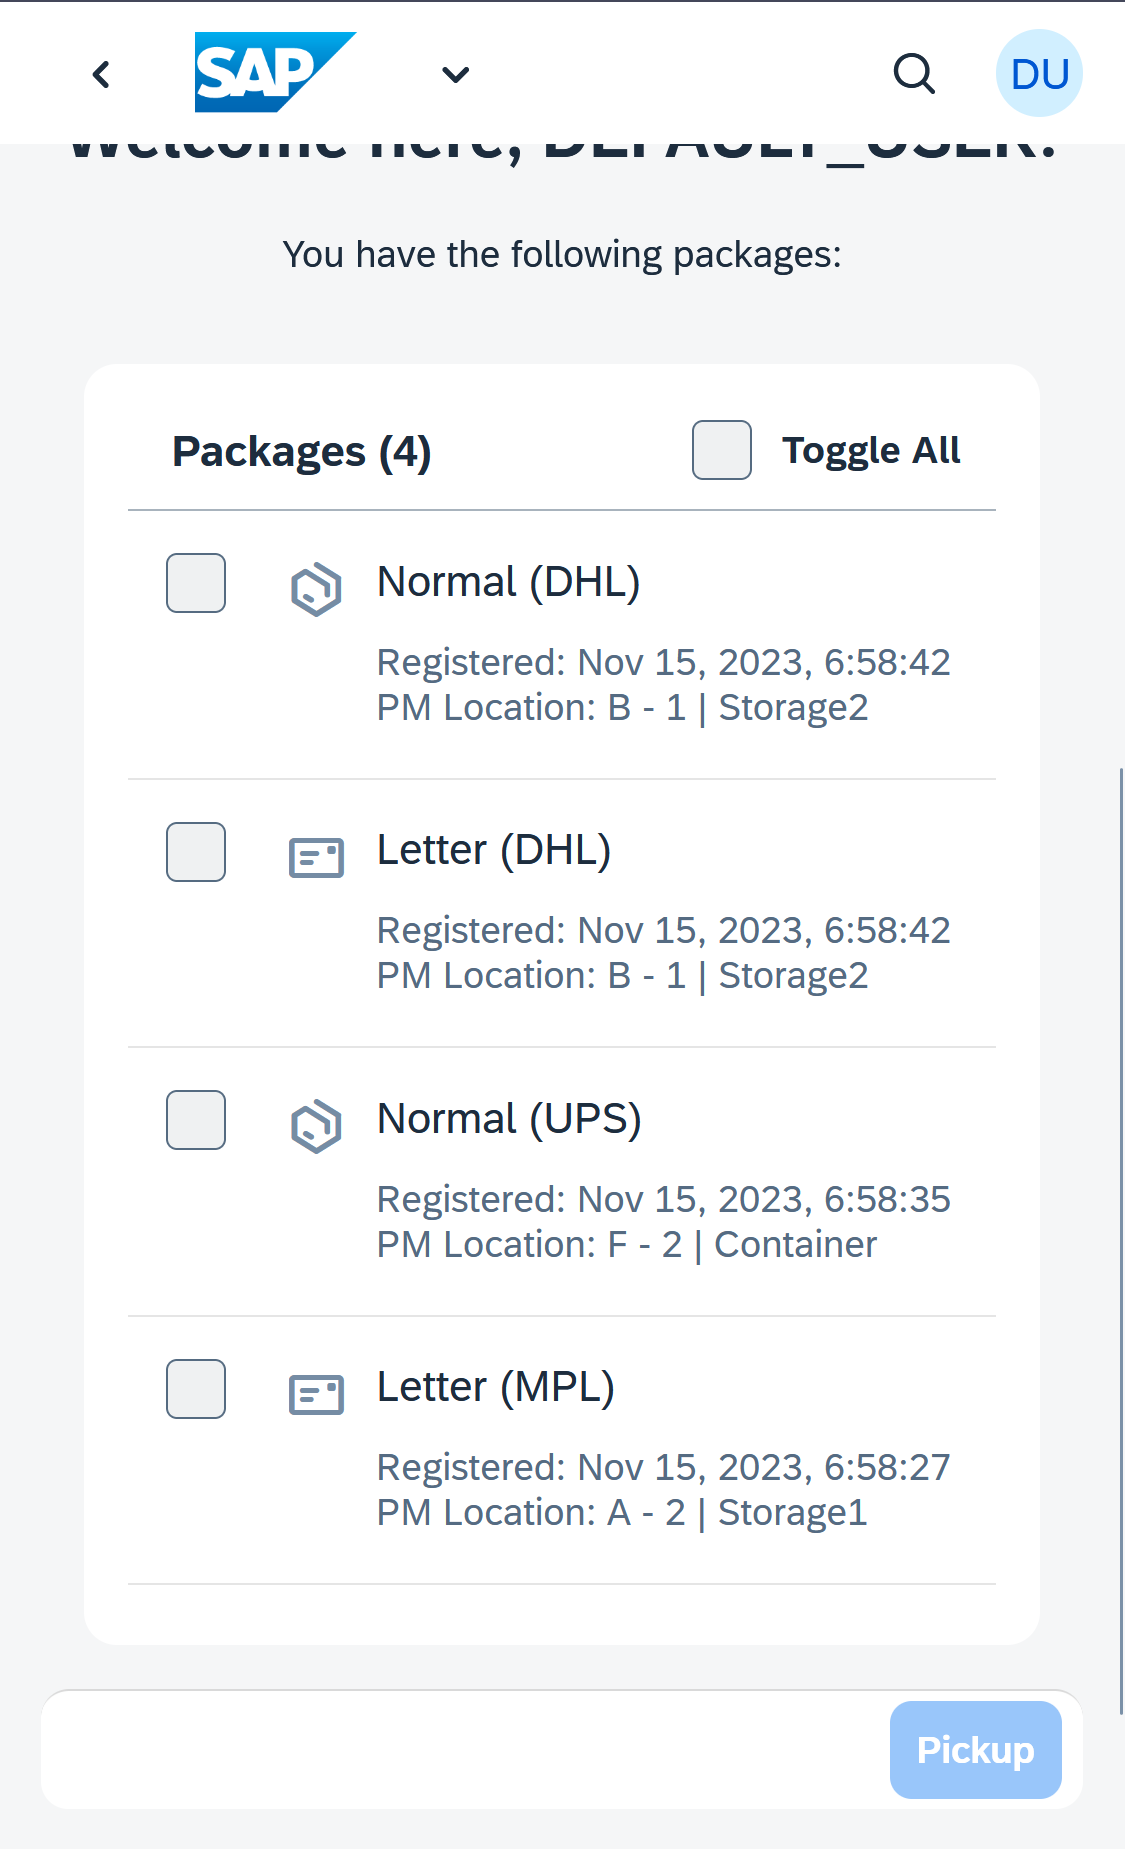
\includegraphics[width=0.45\linewidth]{images/user_doc/pickup/HomeScreenList.png}}
	\hspace{5pt}
	\subcaptionbox{Home Screen without Packages}{
		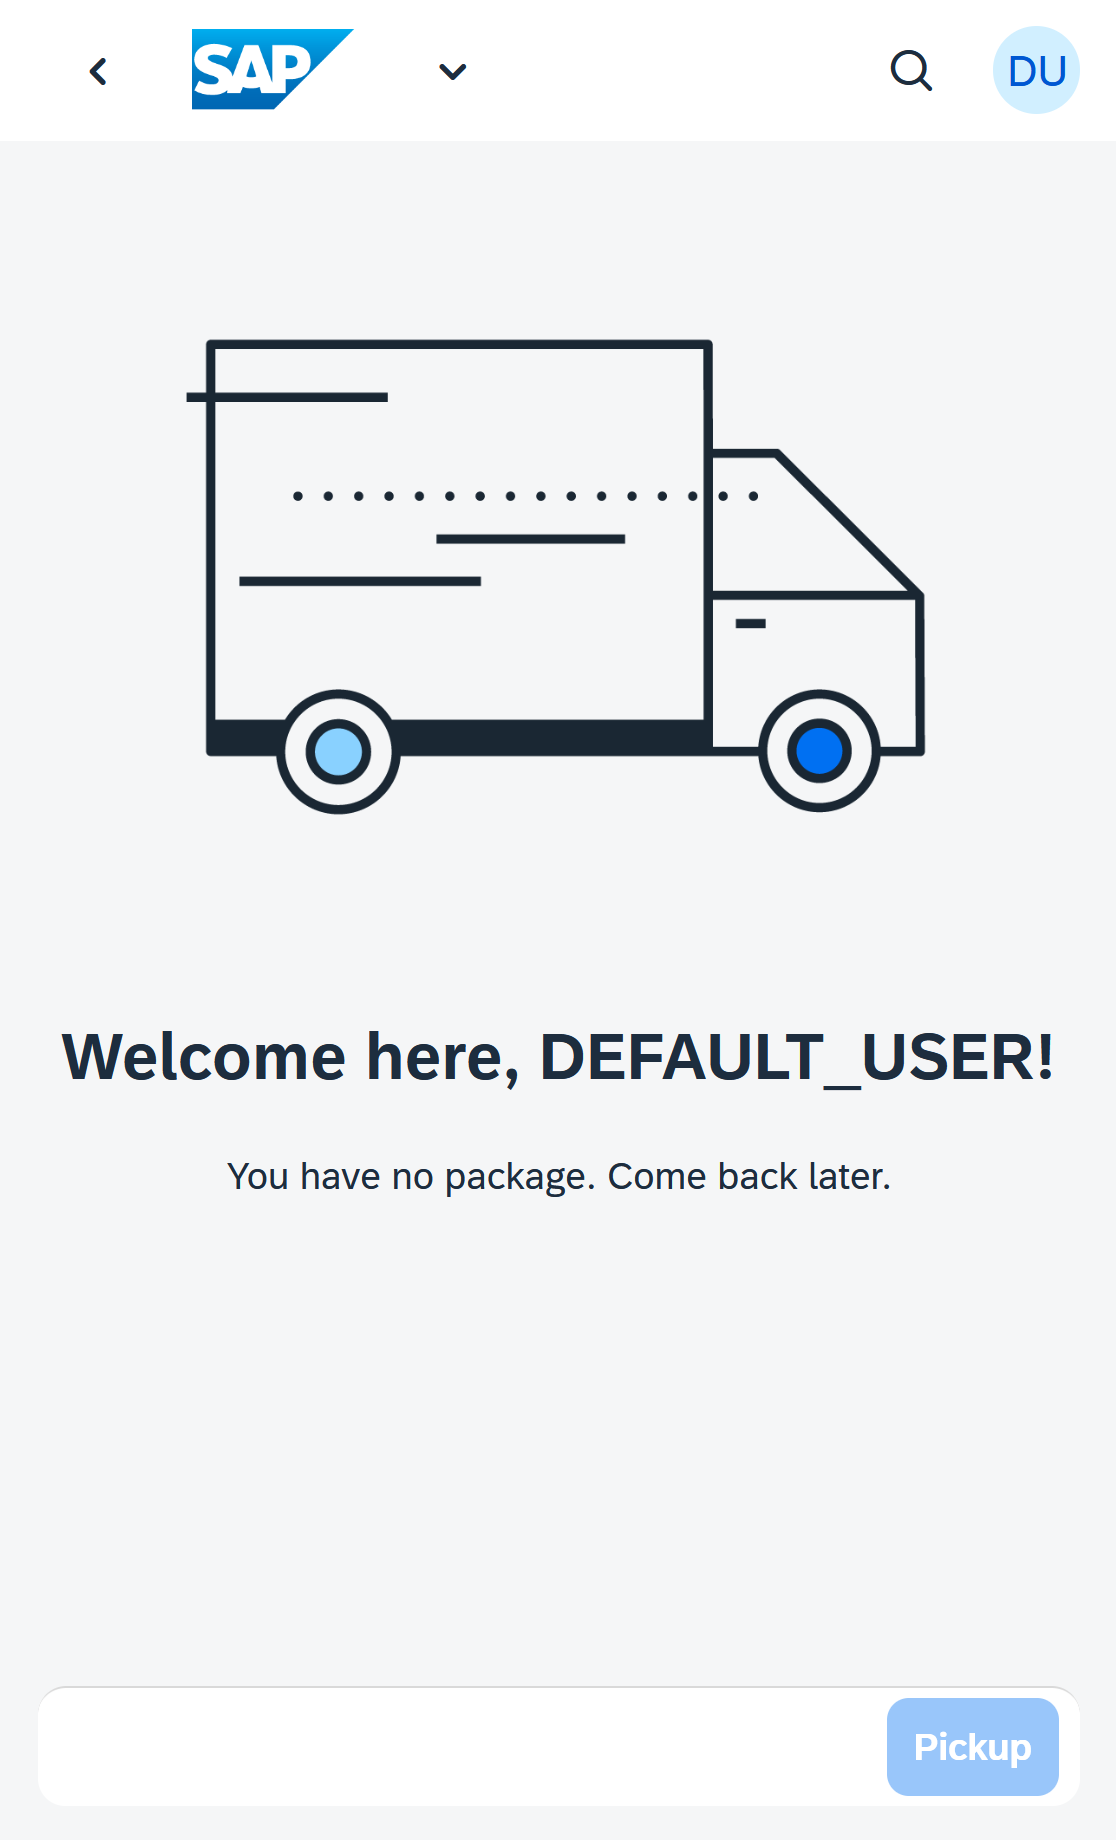
\includegraphics[width=0.45\linewidth]{images/user_doc/pickup/HomeScreenNoPackage.png}}
	\caption{Pickup Home Screen - Package Existence Guide}
	\label{fig:PickupHomeScreen-1}
\end{figure}

\begin{figure}[H]
	\centering
	\subcaptionbox{Home Screen Single Selection}{
		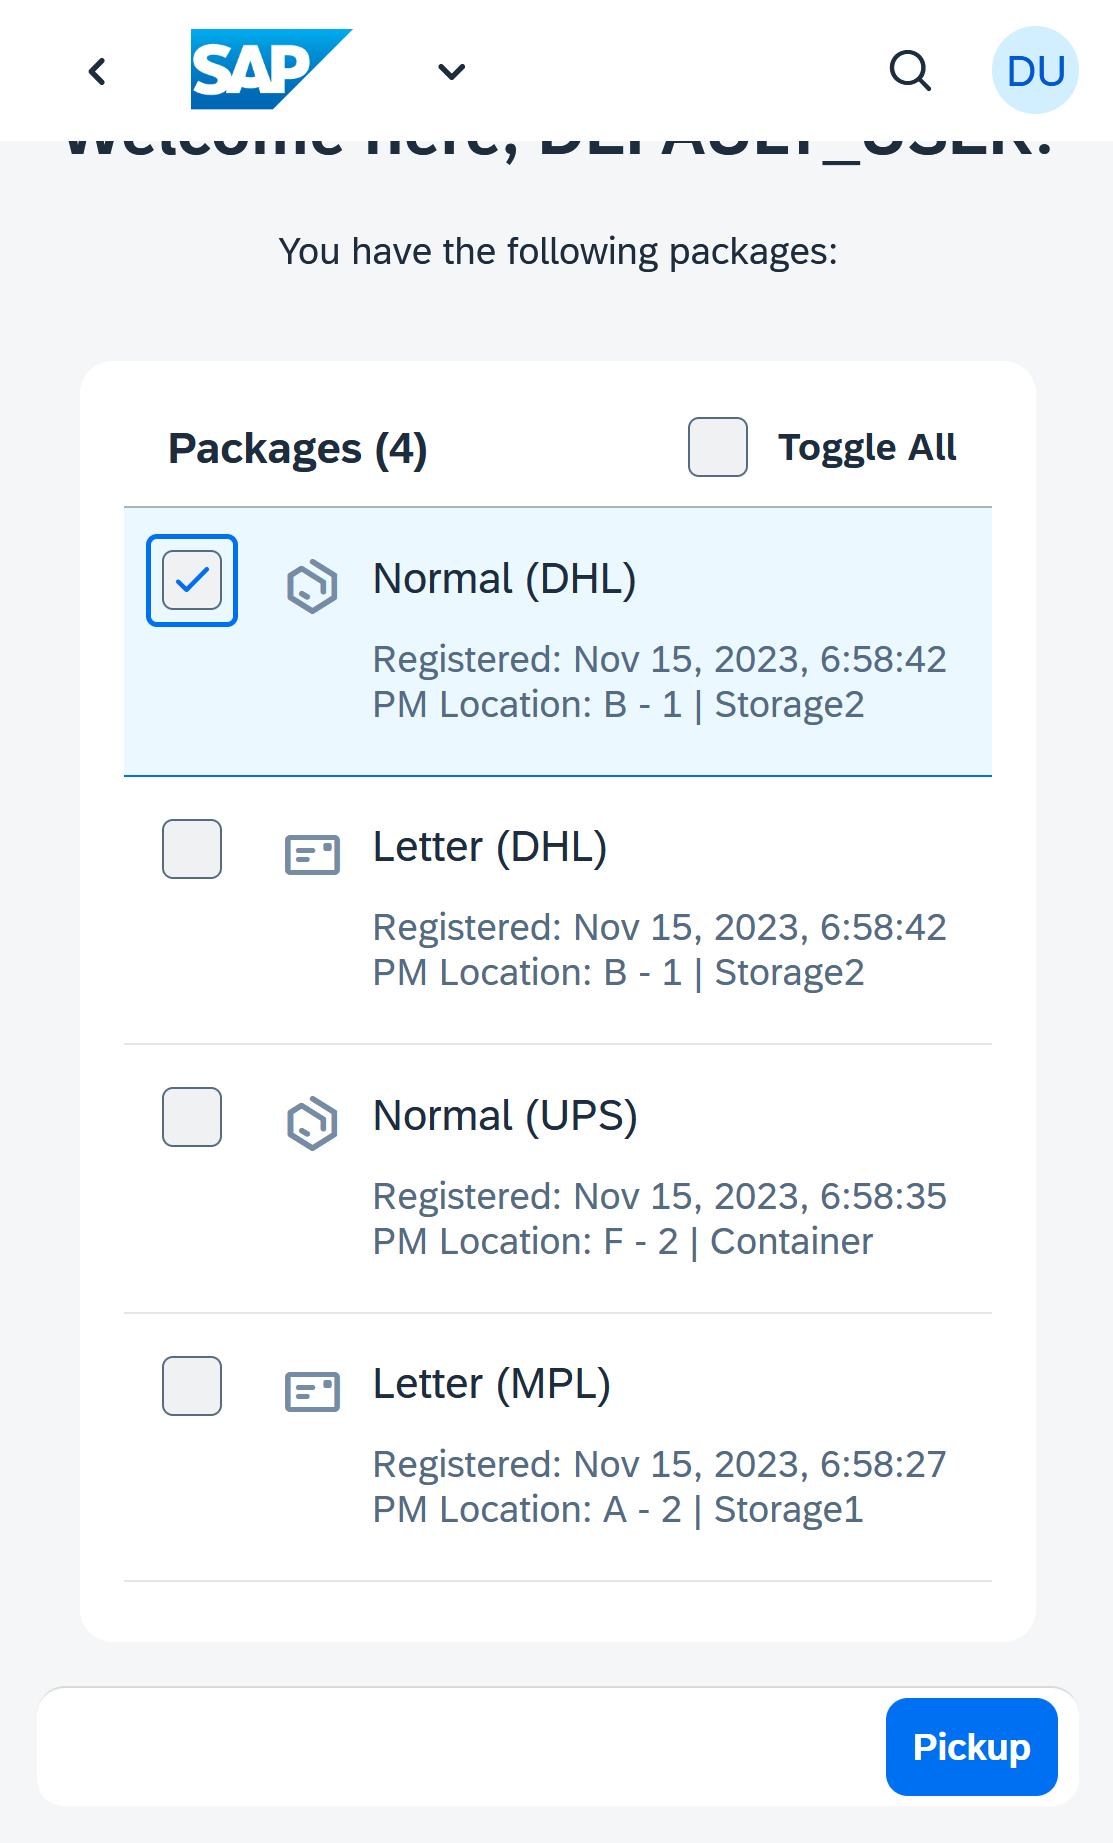
\includegraphics[width=0.45\linewidth]{images/user_doc/pickup/HomeScreenSelectOne.png}}
	\hspace{5pt}
	\subcaptionbox{Home Screen Multiple Selection}{
		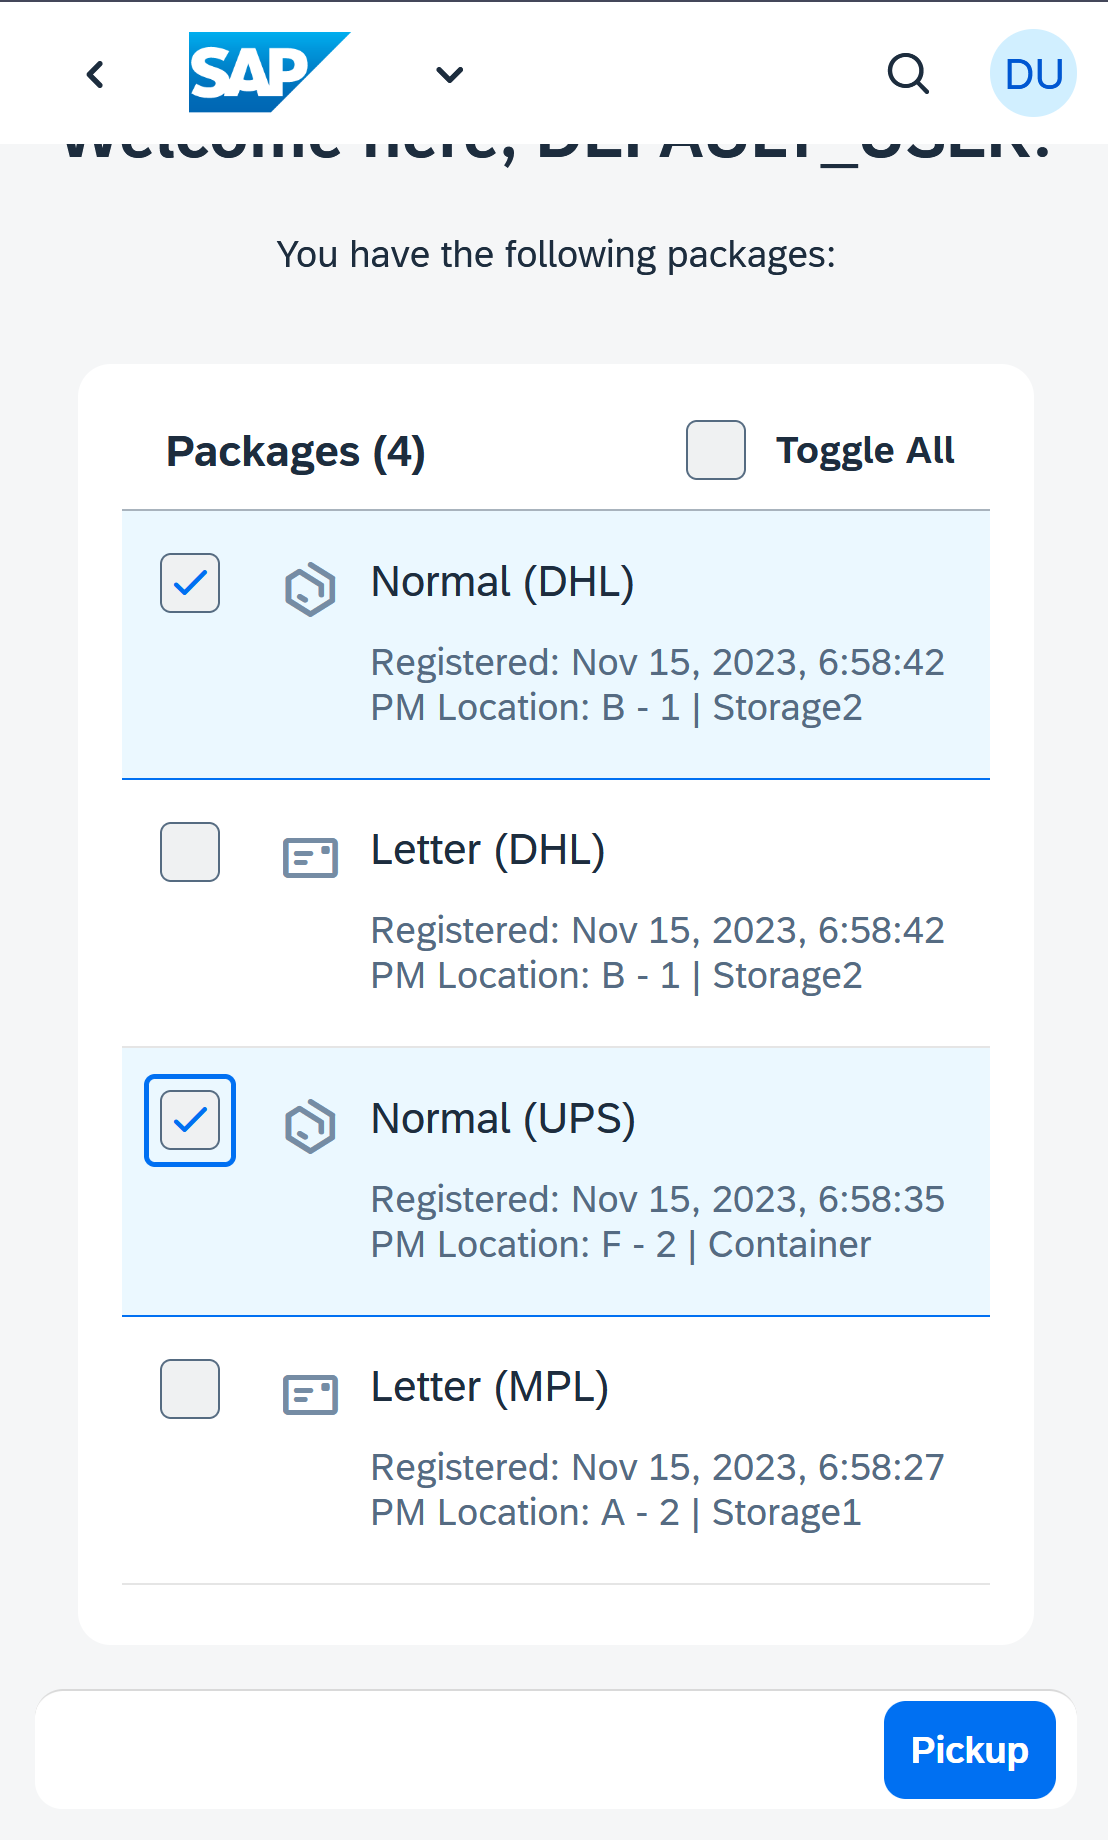
\includegraphics[width=0.45\linewidth]{images/user_doc/pickup/HomeScreenMultiSelect.png}}

    \subcaptionbox{Home Screen Select All}{
		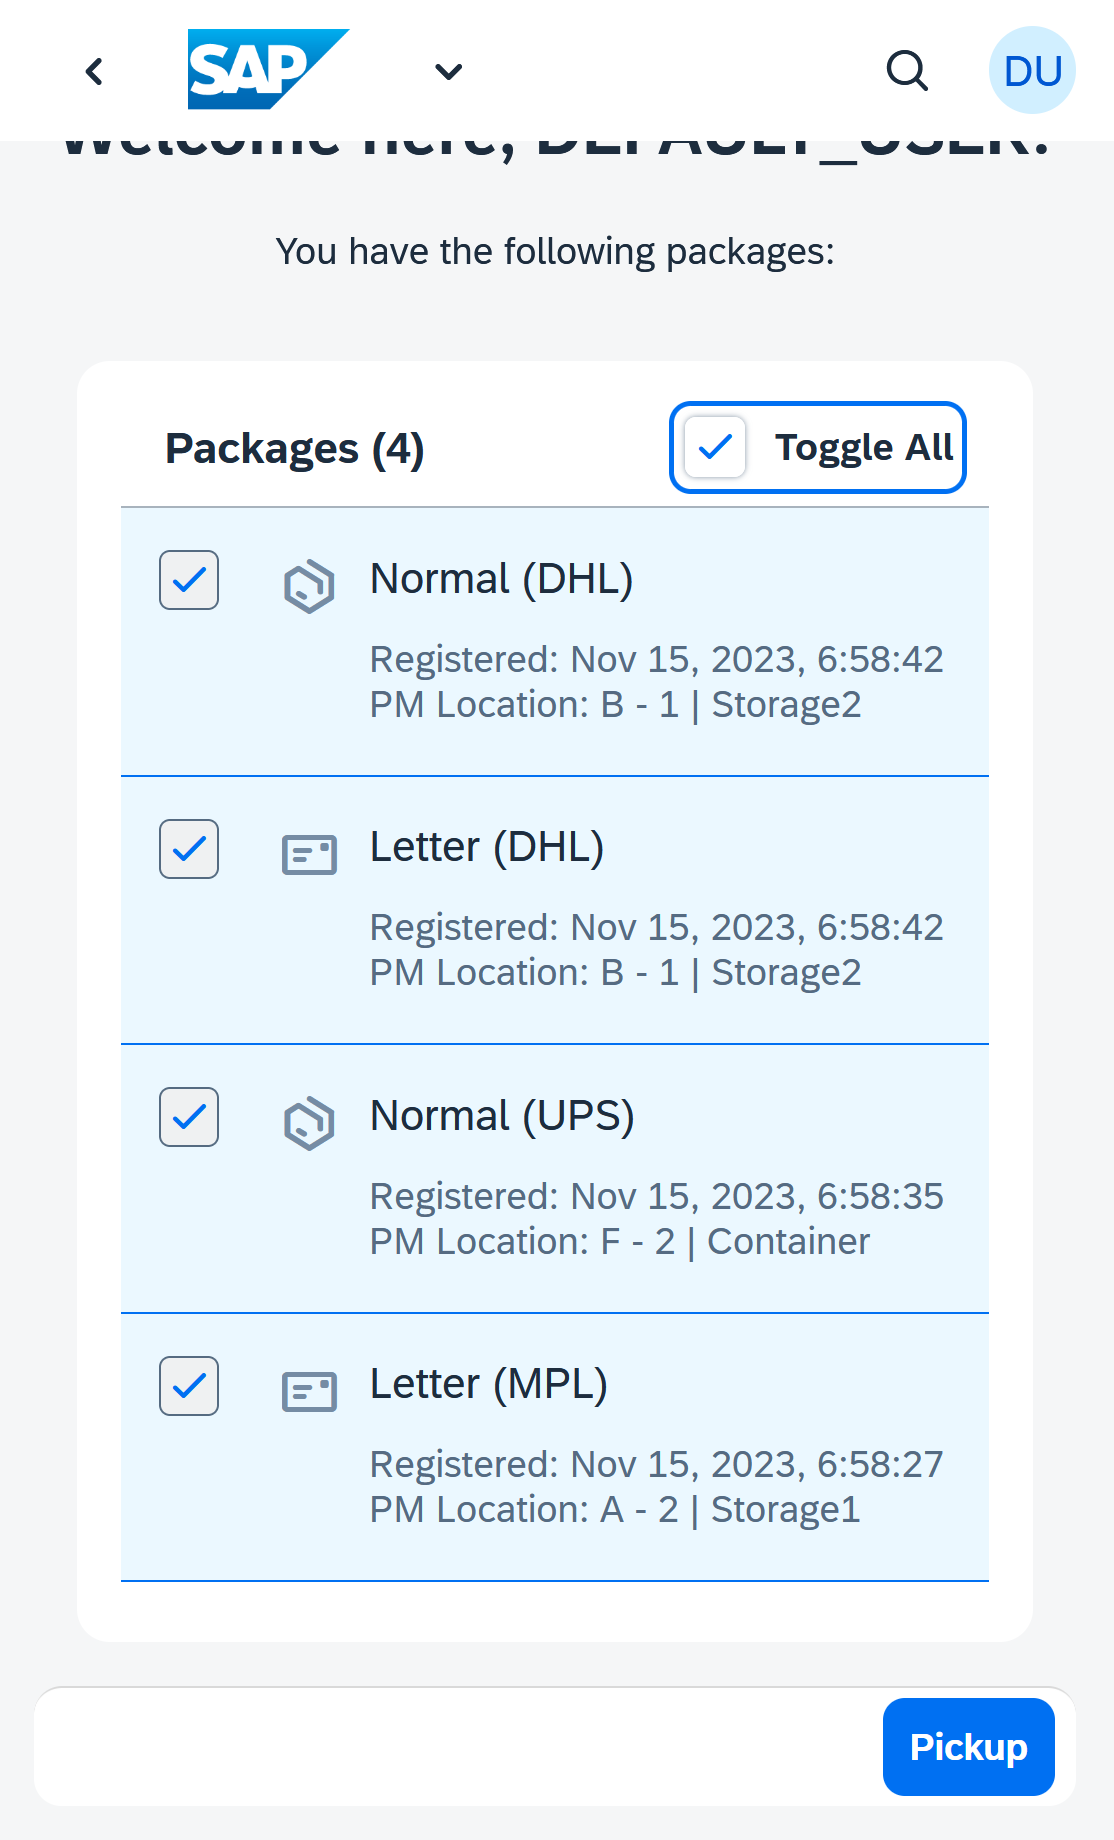
\includegraphics[width=0.45\linewidth]{images/user_doc/pickup/HomeScreenToggleAll.png}}
	\hspace{5pt}
	\subcaptionbox{Home Screen Deselect All}{
		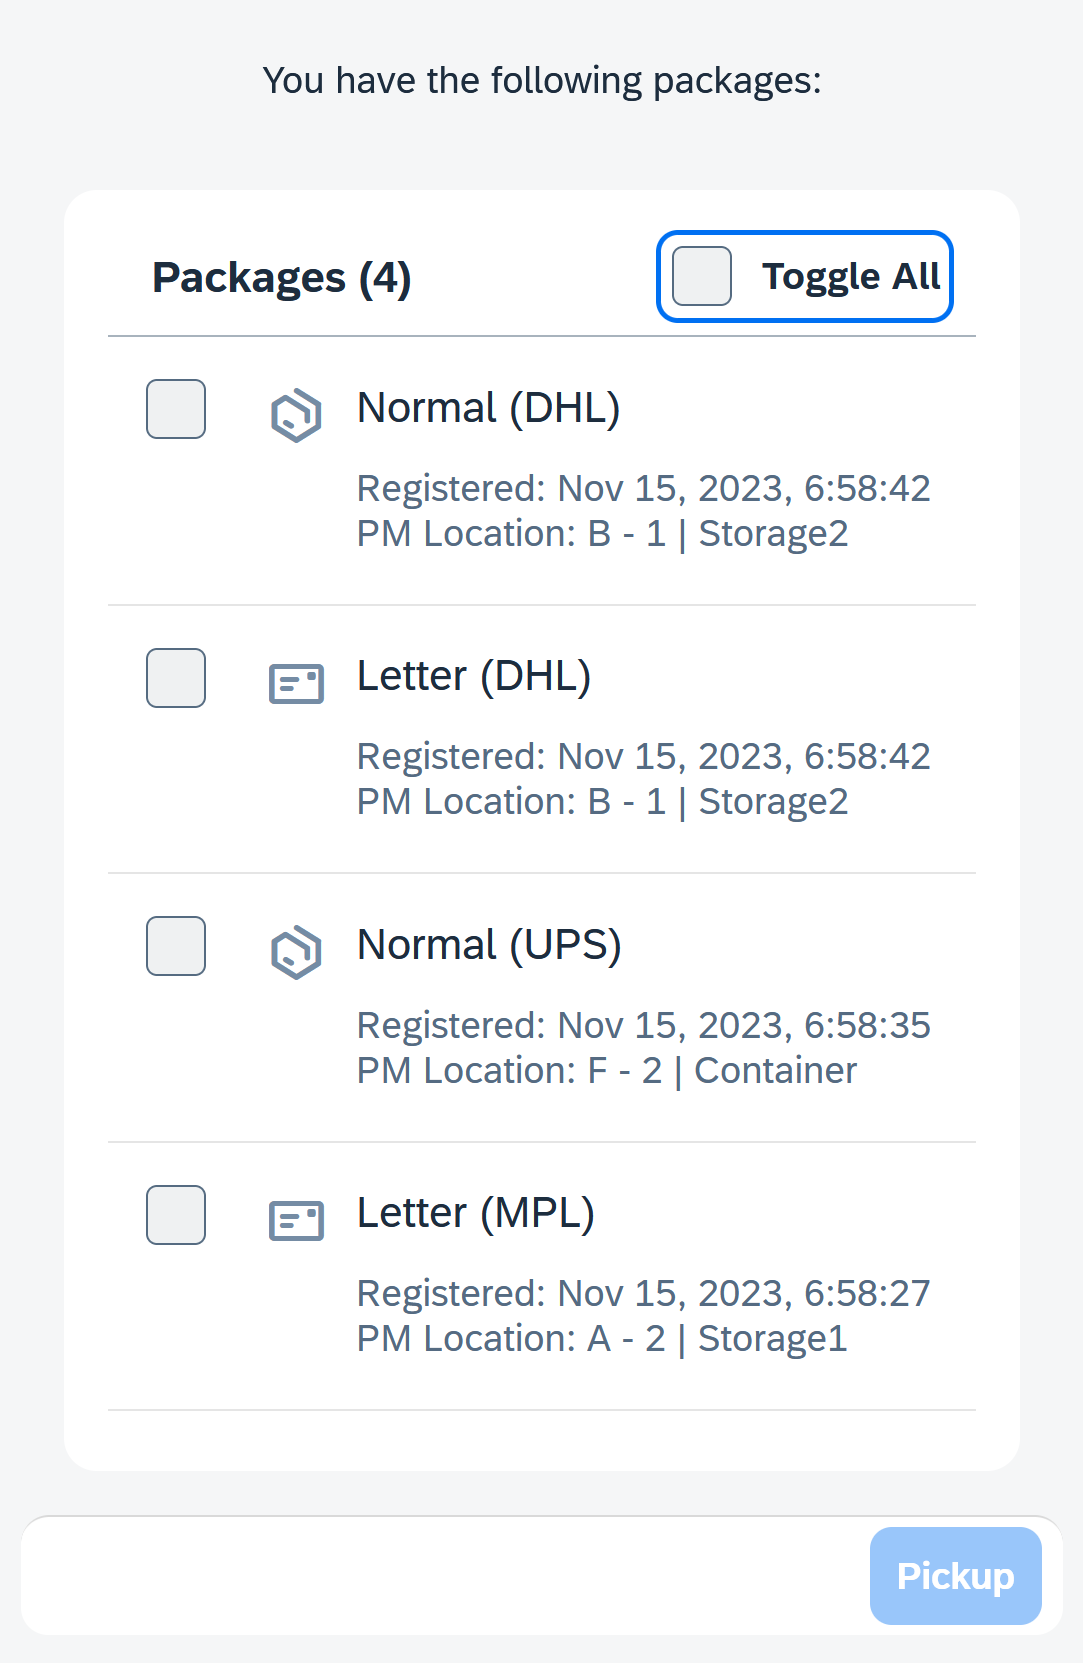
\includegraphics[width=0.45\linewidth]{images/user_doc/pickup/HomeScreenDeToggleAll.png}}
	\caption{Pickup Home Screen - Package Selection Guide}
	\label{fig:PickupHomeScreen-2}
\end{figure}


\subsubsection{Home Screen - Pickup}
The "Pickup" button at right bottom corner will only be enabled if at least one package is selected. In case it is enabled, one can pick up the selected packages by left clicking the "Pickup" button, which will trigger a confirmation dialog. If one choose "Cancel", the dialog closes and no modification is made. If one choose "OK", then all packages selected will be marked as pickup, removed from the list and the user will be navigated to the "Done Screen". At this point, the process of the picked up package will be closed, the package data will never be deleted and \textbf{End User} can always go to \textbf{My Packages} application to check the package history. (figure \ref{fig:PickupDialog})

\begin{figure}[H]
	\centering
	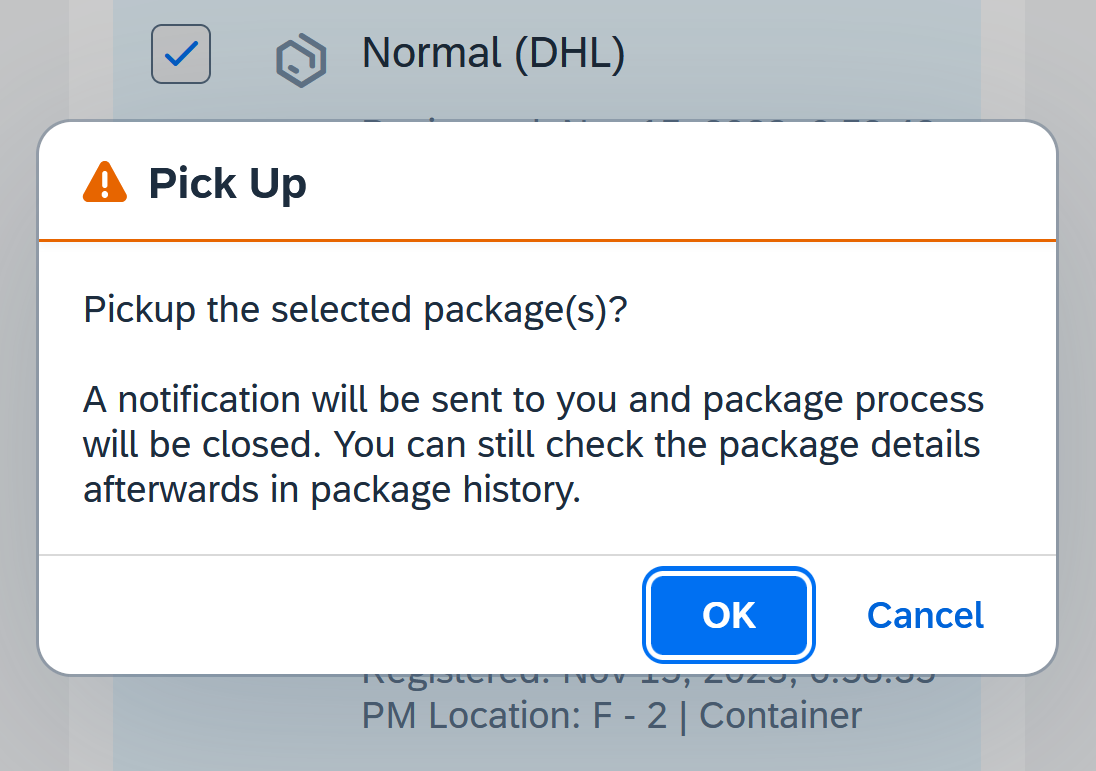
\includegraphics[height=200pt]{images/user_doc/pickup/PickupDialog.png}
	\caption{Pickup Home Screen - Pickup Dialog}
	\label{fig:PickupDialog}
\end{figure}


\subsubsection{Done Screen}

At the "Done Screen", if the \textbf{End User} still have packages to pickup, it will display the list of packages showing their \textbf{type with icon}, \textbf{delivery company} and \textbf{location info}. Otherwise, it displays no more packages. 
User can always navigate back to "Home Screen" by left clicking the "Close" button at the right bottom corner of the page.
From there, a new pickup iteration starts.
(figure \ref{fig:PickupDoneScreen-1})

\begin{figure}[H]
	\centering
	\subcaptionbox{Done Screen with Packages}{
		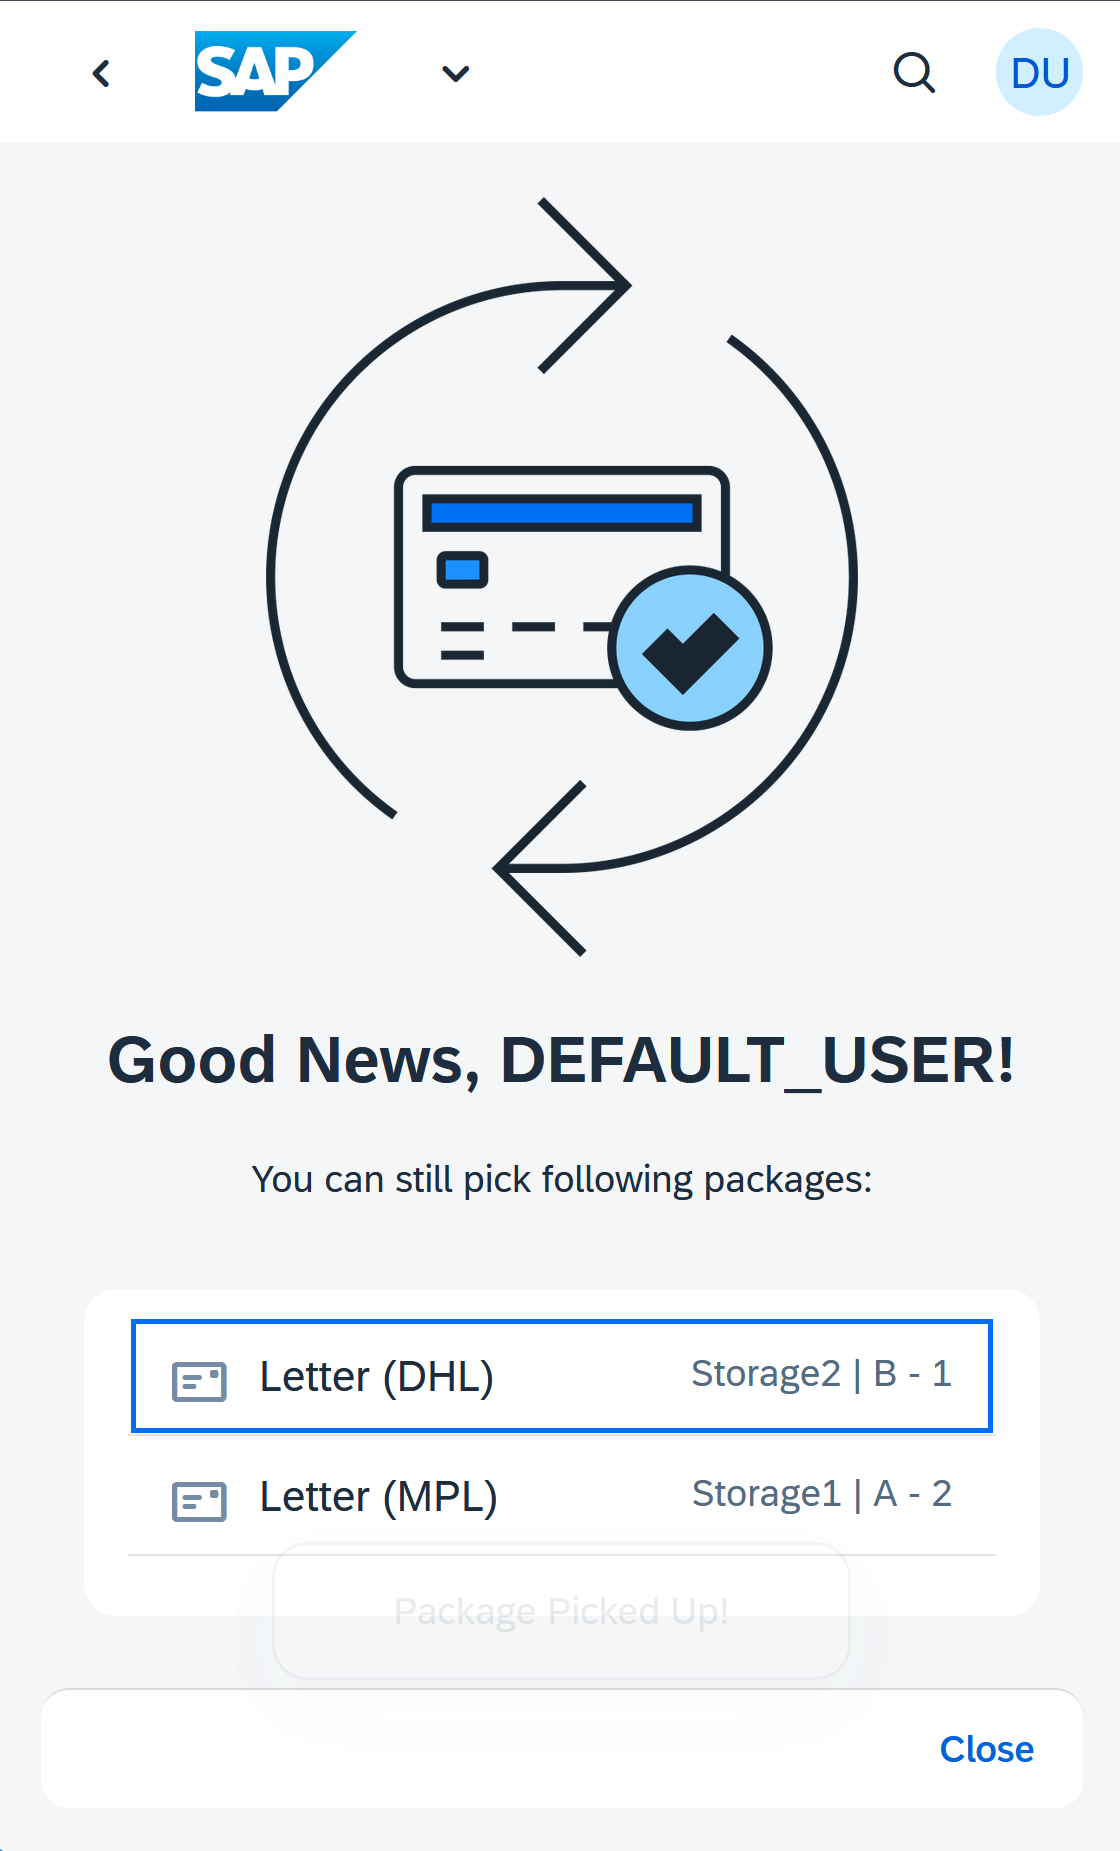
\includegraphics[width=0.45\linewidth]{images/user_doc/pickup/DoneScreenRemainPackages.png}}
	\hspace{5pt}
	\subcaptionbox{Done Screen without Packages}{
		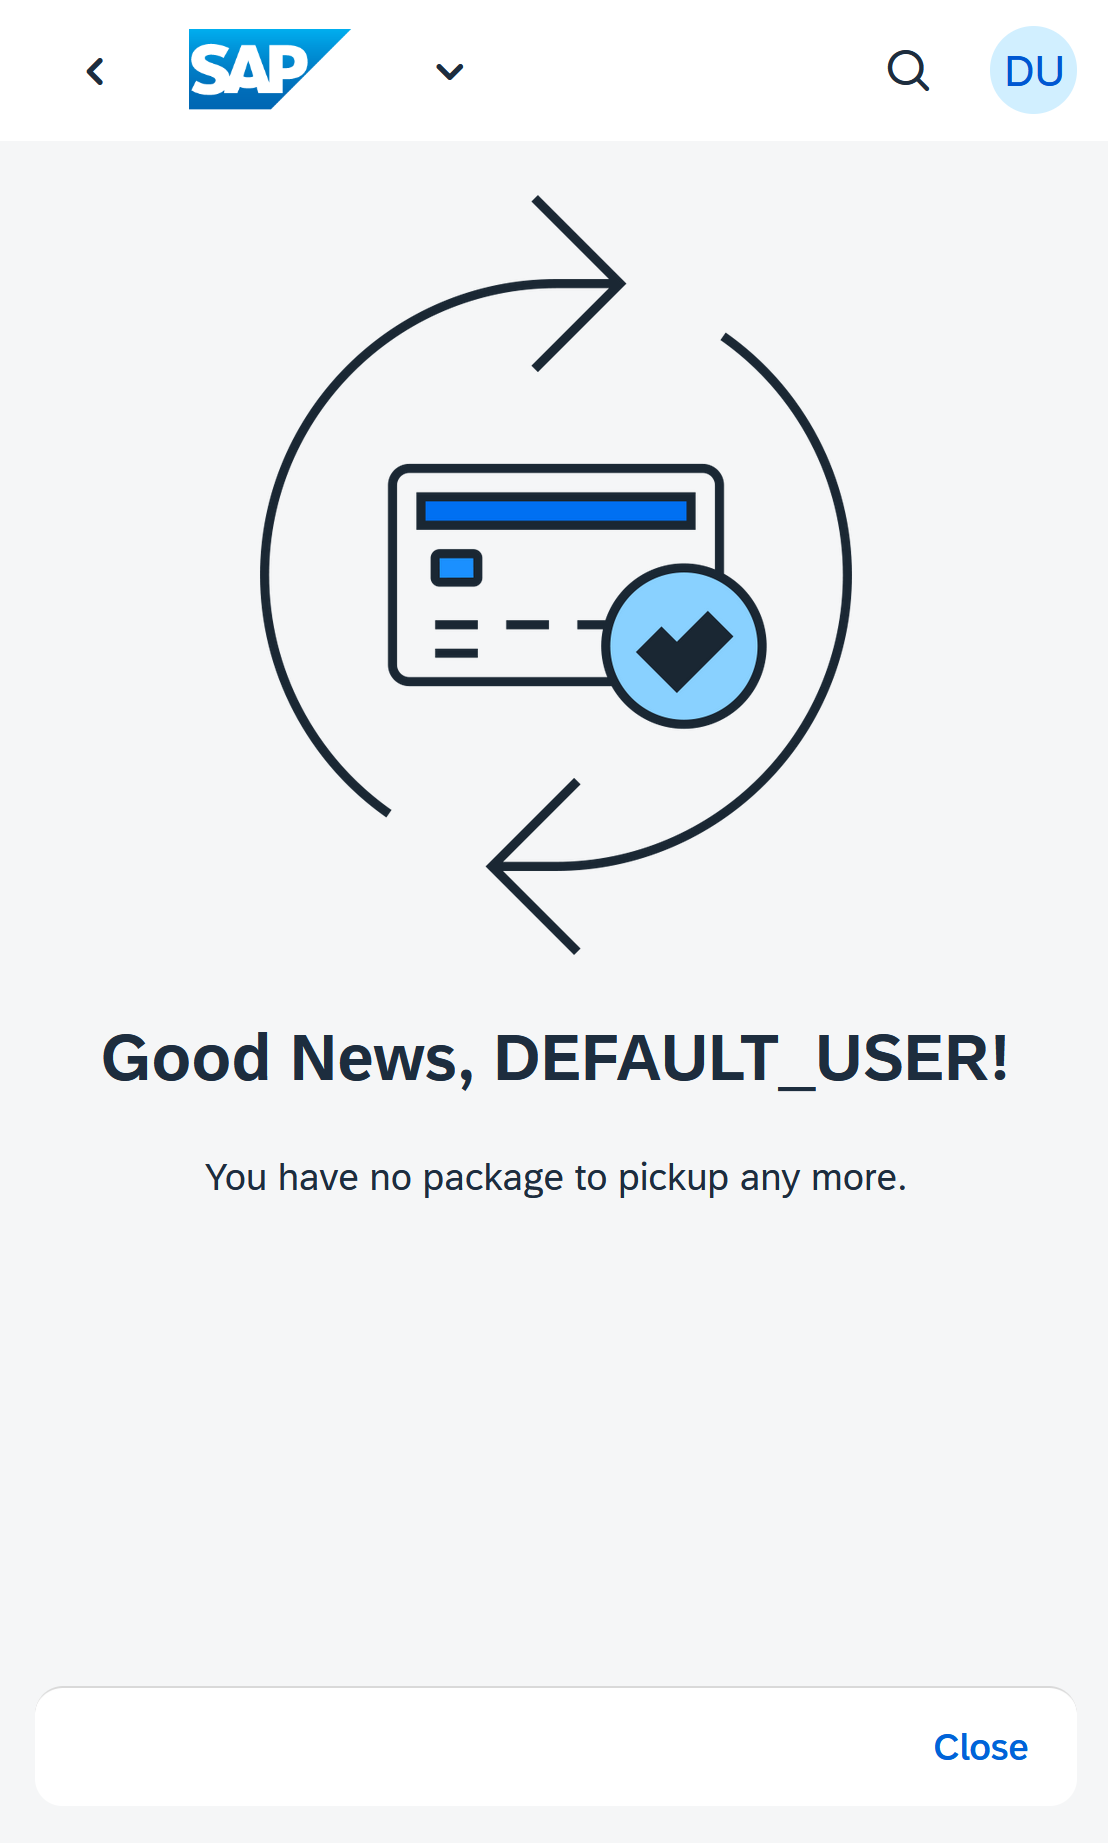
\includegraphics[width=0.45\linewidth]{images/user_doc/pickup/DoneScreenNoPackage.png}}
	\caption{Pickup Done Screen - Package Existence Guide}
	\label{fig:PickupDoneScreen-1}
\end{figure}

\pagebreak

\section{Receptionist}
\label{sec:UdocReceptionist}

As a logged in \textbf{Receptionist} (See \autoref{sec:GeneralRequisite} for all possible roles), one is granted to access the two applications under the \textbf{Parcel Handling} section, namely \textbf{Register Packages} (\autoref{subsec:rp}) and \textbf{Manage Packages} (\autoref{subsec:mp}). One can quick jump to the section by left clicking the "Parcel Handling" tab. One can enter the application by left click the tiles. (\autoref{fig:PHApplications})

\begin{figure}[H]
	\centering
	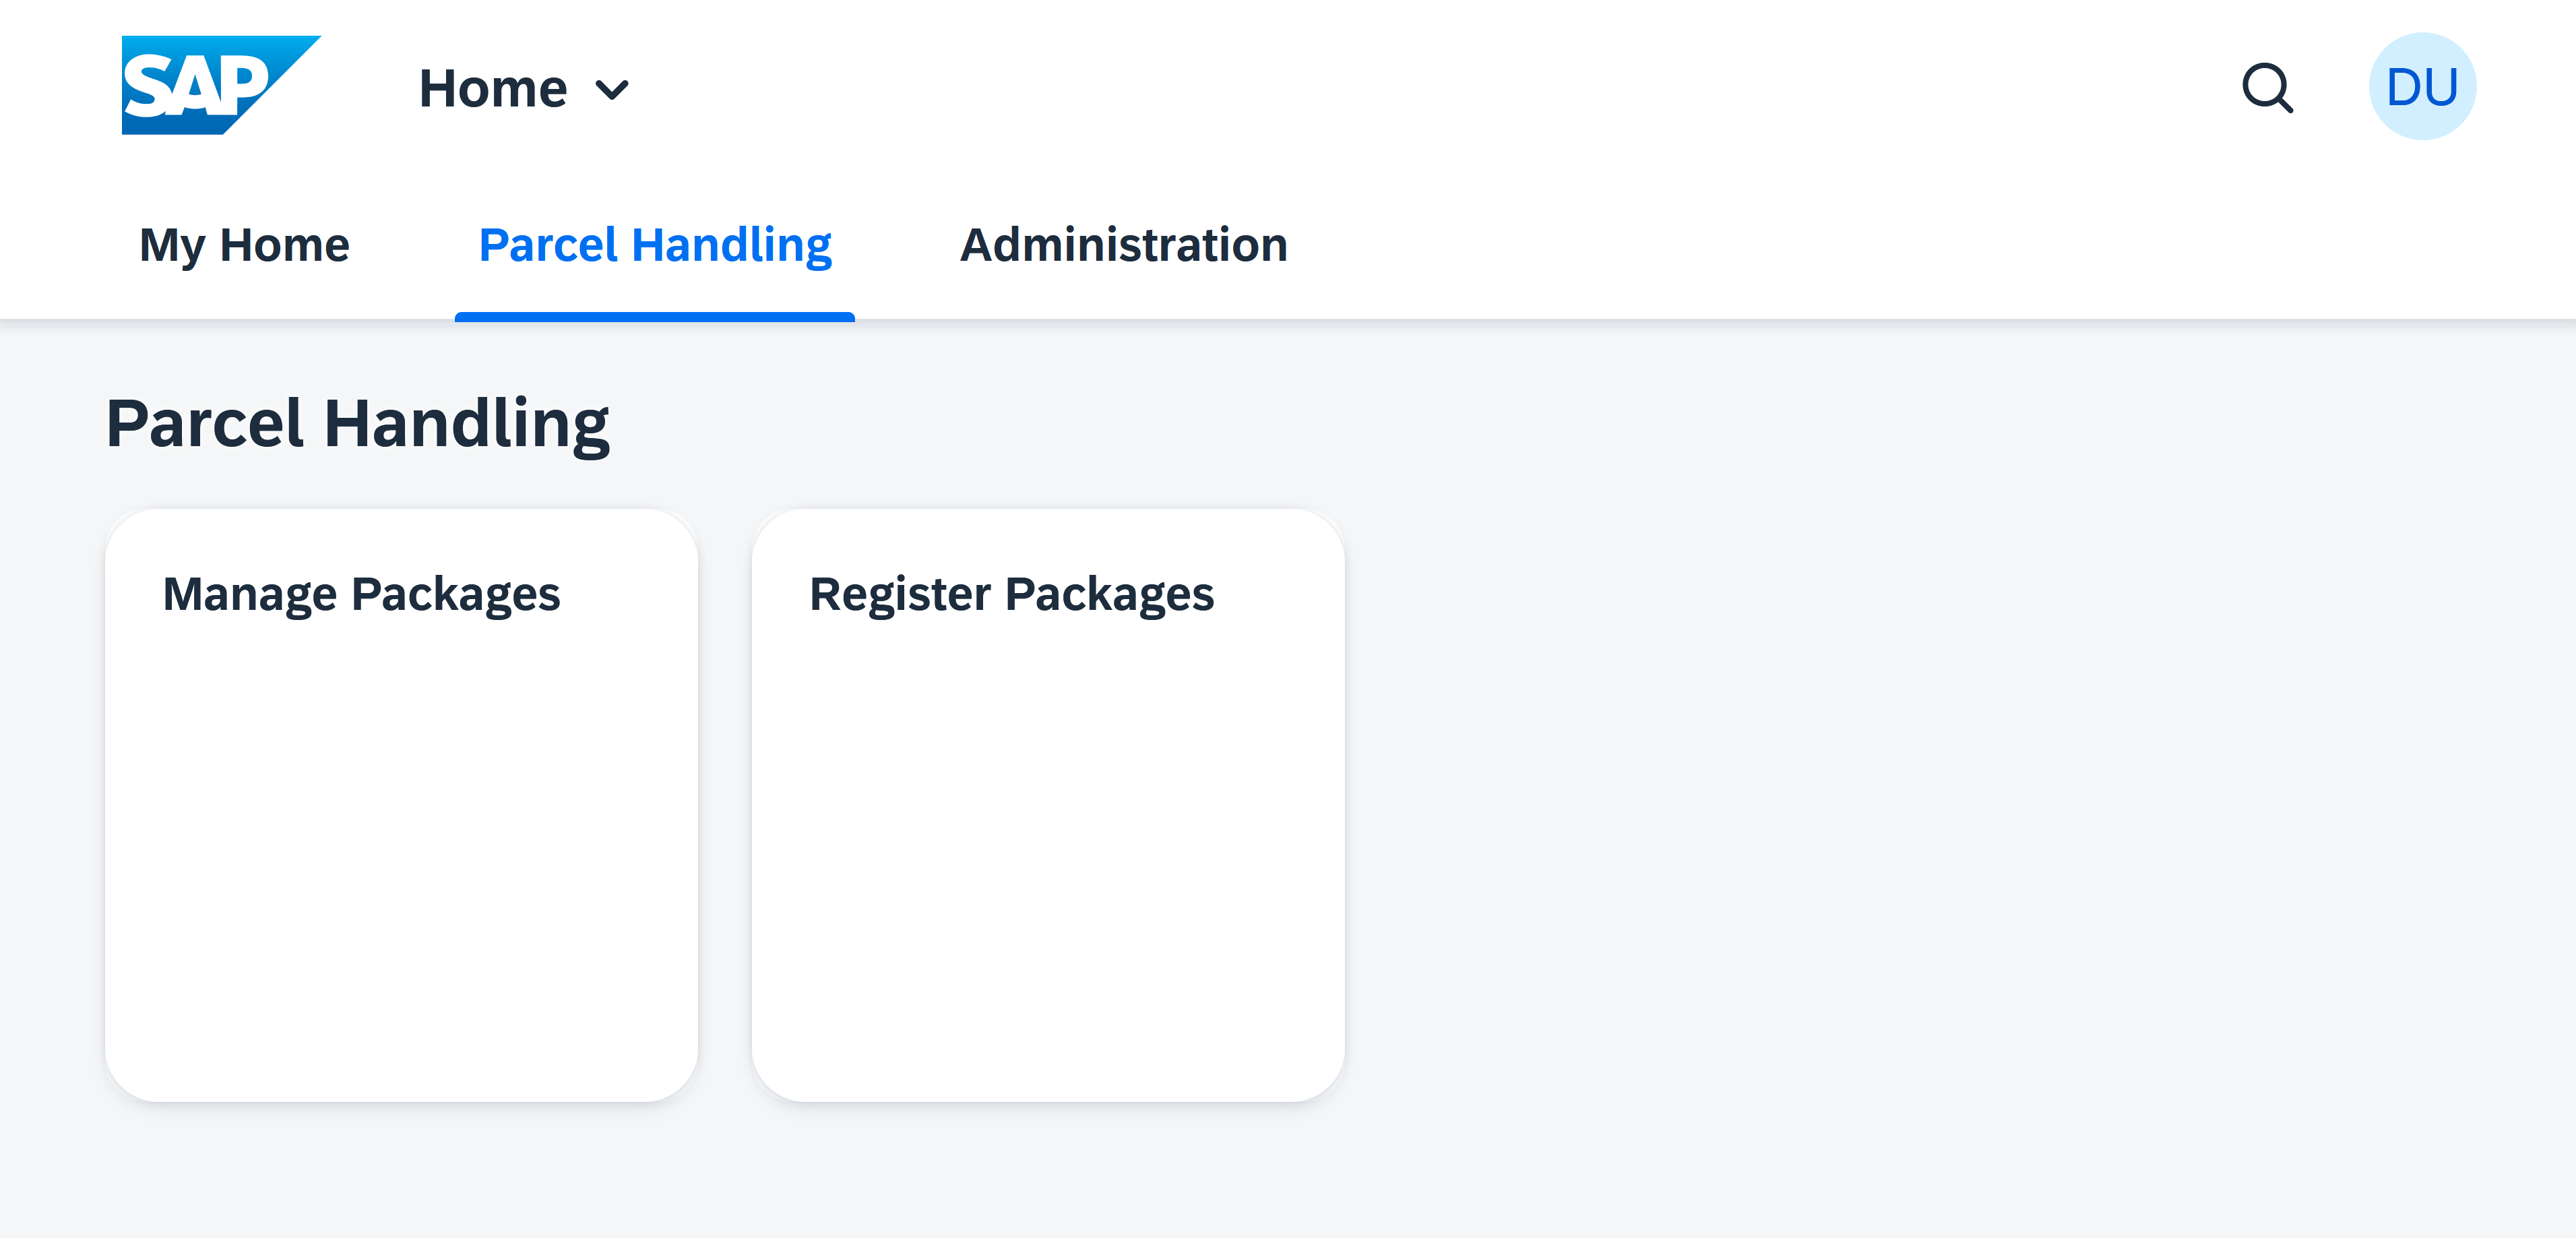
\includegraphics[width=1\linewidth]{images/user_doc/overviews/ParcelHandlingTab.png}
	\caption{Parcel Handling Applications}
	\label{fig:PHApplications}
\end{figure}


\subsection{Register Packages}
\label{subsec:rp}

When the delivery person arrived at the reception with the new parcels, the \textbf{Receptionist} shall use \textbf{Register Packages} application to register the newly arrived parcels into the system. (See \autoref{sec:UdocReceptionist} for all receptionist related applications) After the registration, \textbf{Receptionist} will be automatically redirected to  \textbf{Manage Packages}.
The summarized main actions the \textbf{Receptionist} can take within the application are listed here:

\begin{compactenum}
	\item Register a newly arrived package.
    \item Register multiple newly arrived packages.
    \item Discard current registration.
\end{compactenum}

\subsubsection{Data Entry}

As an \textbf{Receptionist}, by clicking at the \textbf{Register Packages} application tile, is redirected to the "Registration Form" (\autoref{fig:RPOverview}), which is the main and only screen of this application. At this point, \textbf{Recipient}, \textbf{Type}, \textbf{} and optionally \textbf{Comment} of the package are required by the form. (\autoref{fig:RPformEntry})

\begin{figure}[H]
	\centering
	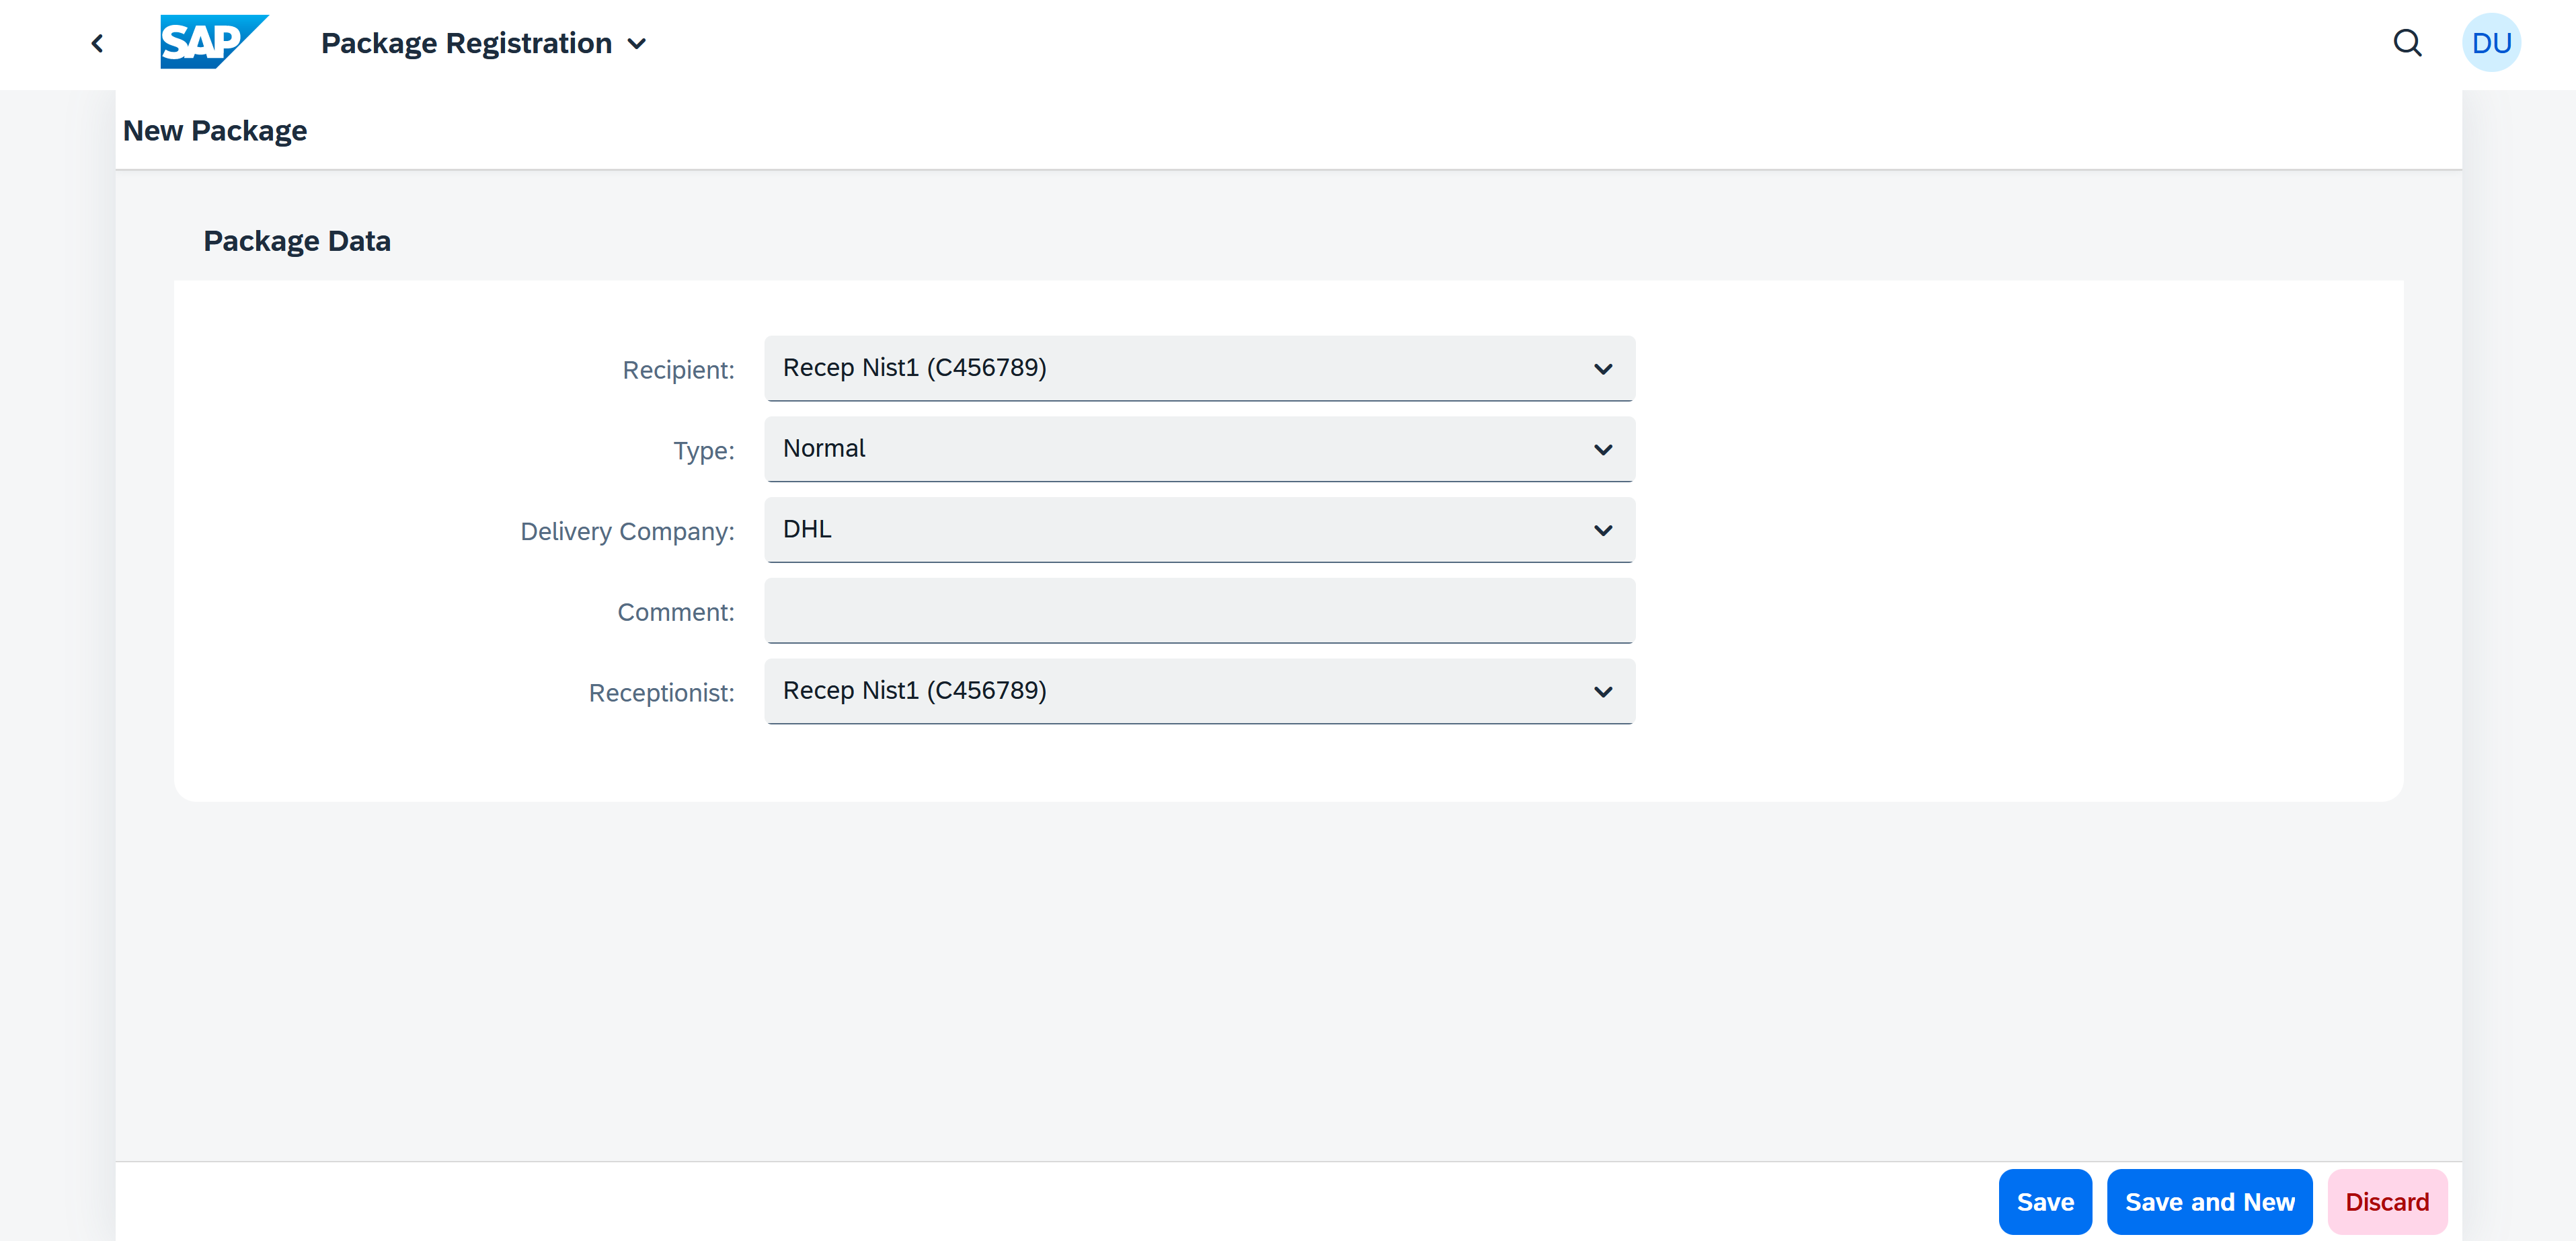
\includegraphics[width=1\linewidth]{images/user_doc/registration/overview.png}
	\caption{Register Packages Form - Overview}
	\label{fig:RPOverview}
\end{figure}


\begin{figure}[H]
	\centering
	\subcaptionbox{Step 1: Choose Recipient}{
		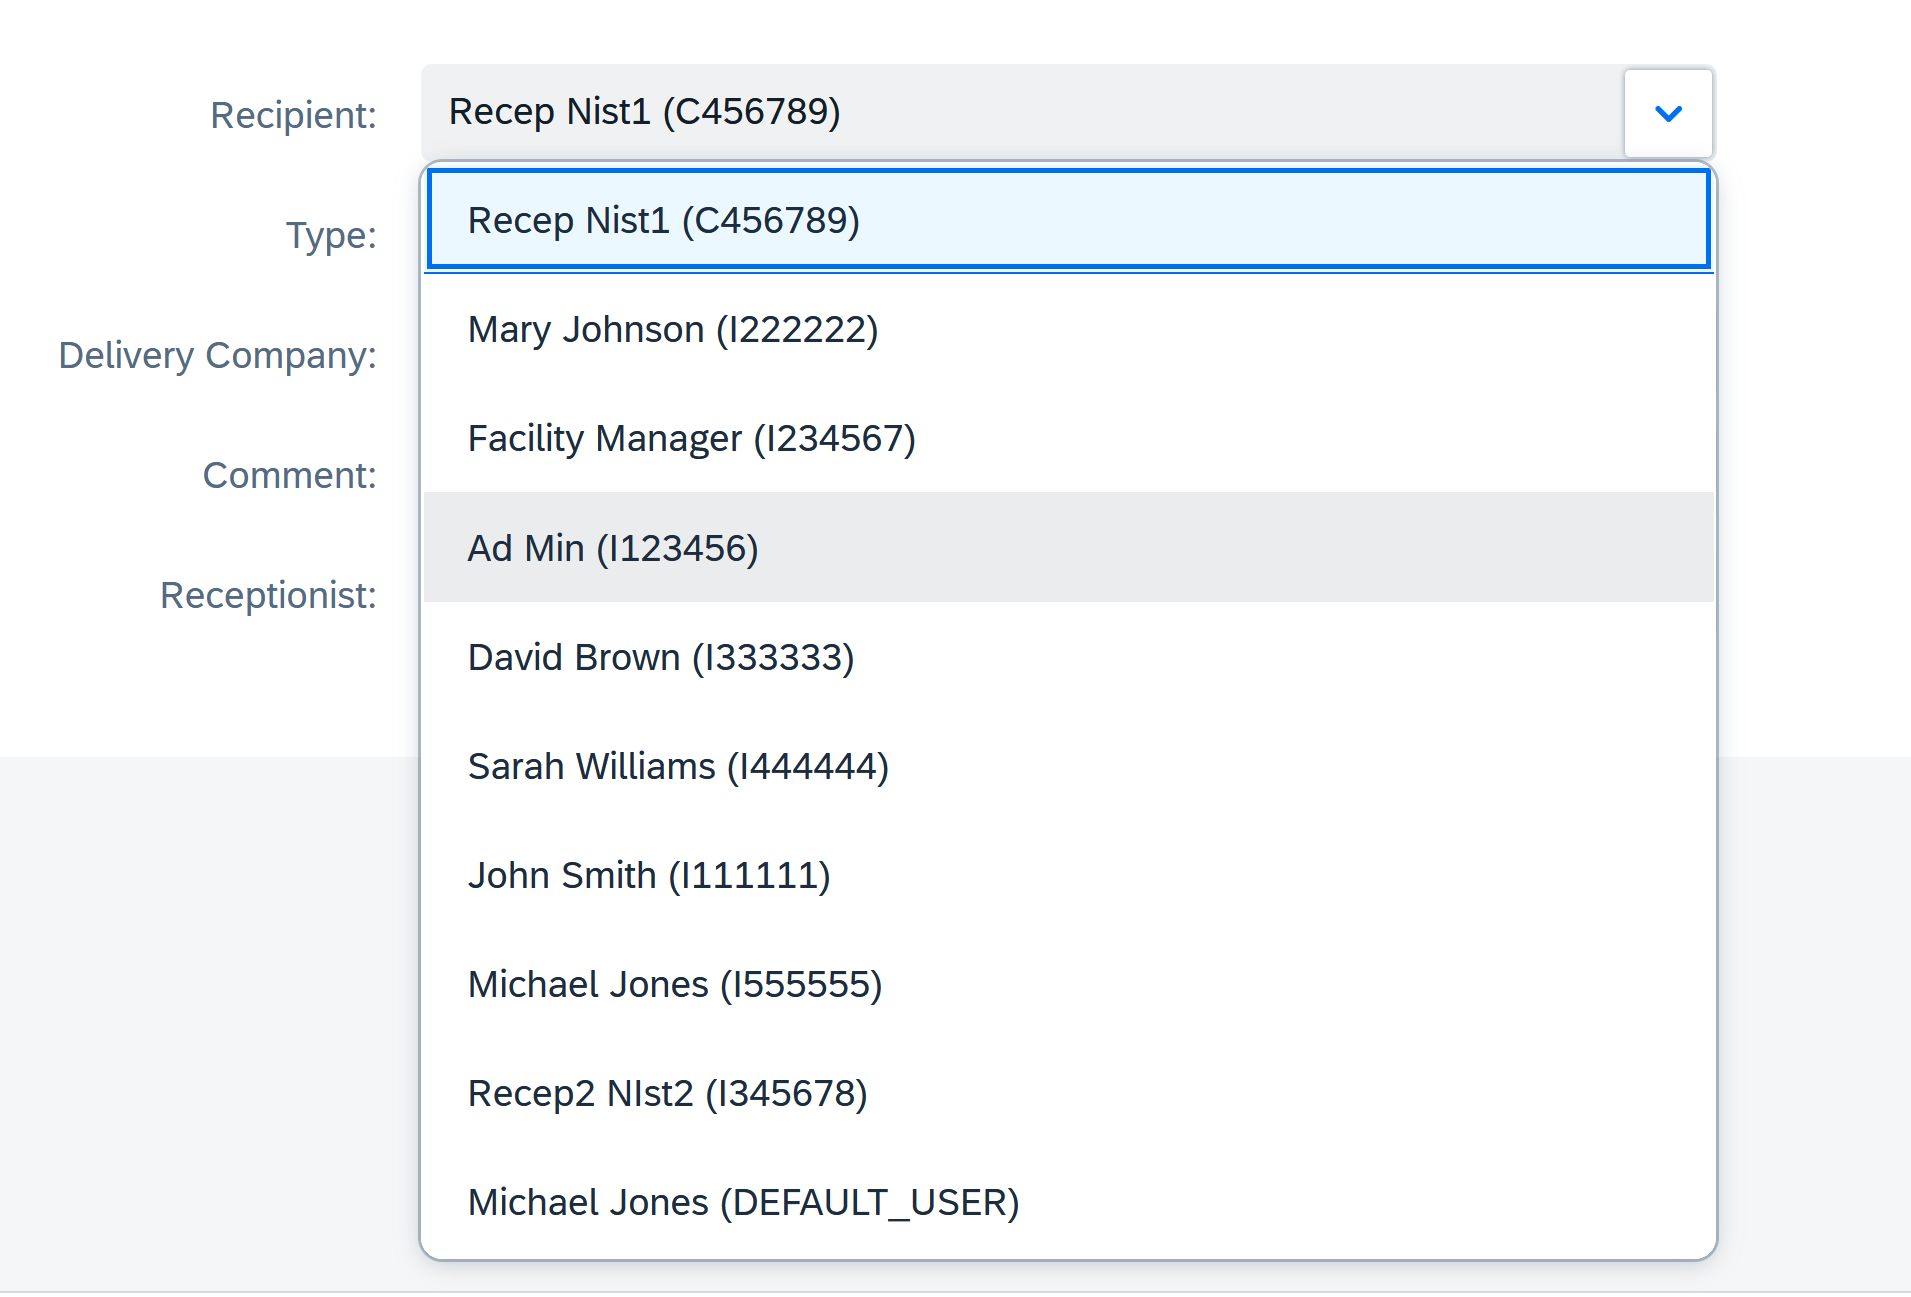
\includegraphics[width=0.45\linewidth]{images/user_doc/registration/entry1.png}}
   \hspace{5pt}
    \subcaptionbox{Step 2: Choose Package Type}{
		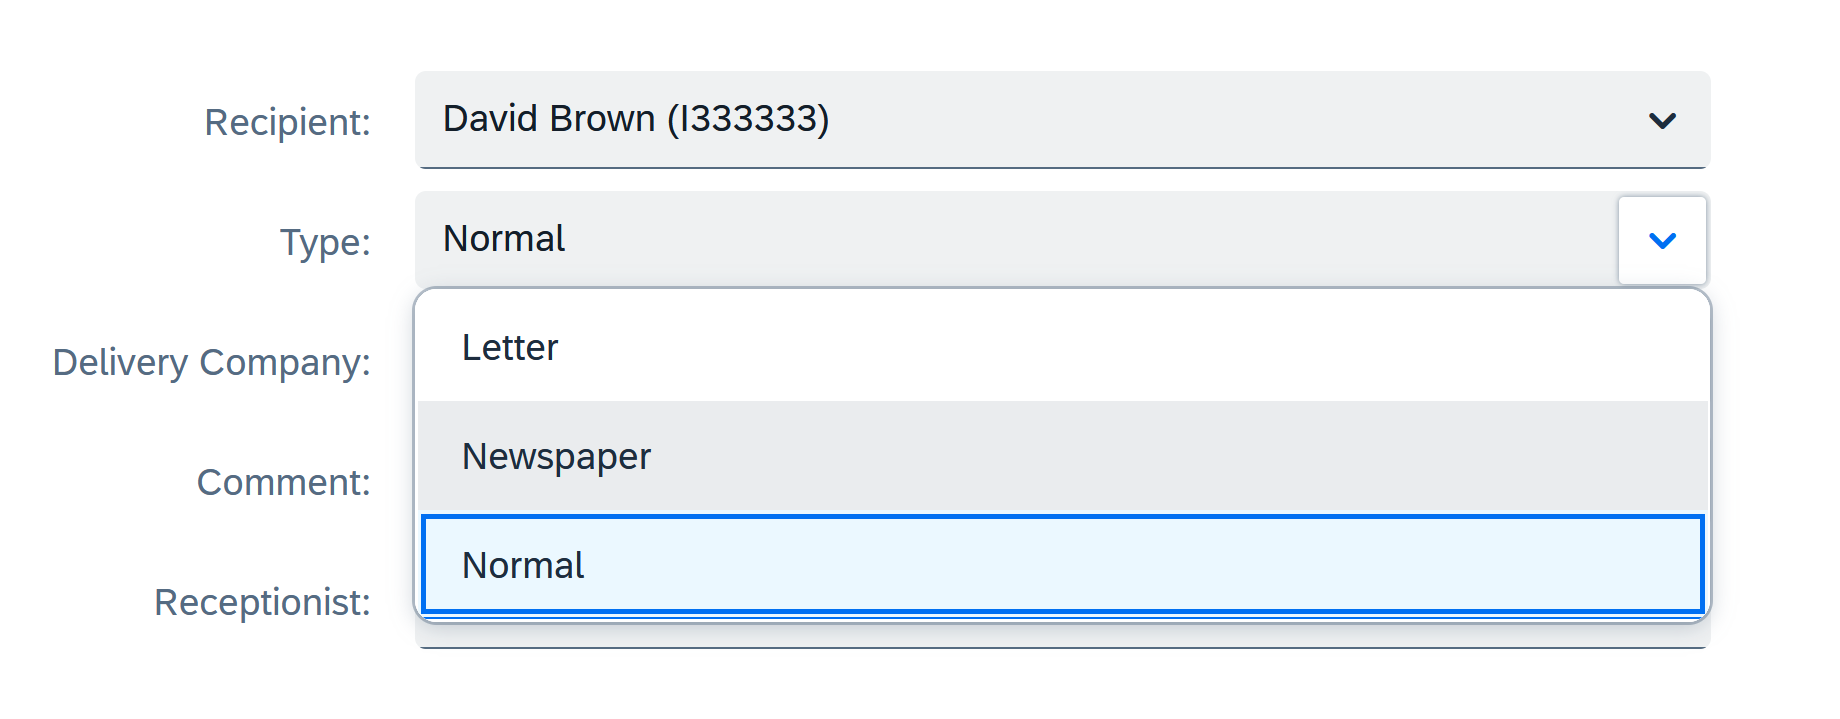
\includegraphics[width=0.45\linewidth]{images/user_doc/registration/entry2.png}}
  
	\subcaptionbox{Step 3: Choose Delivery Company}{
		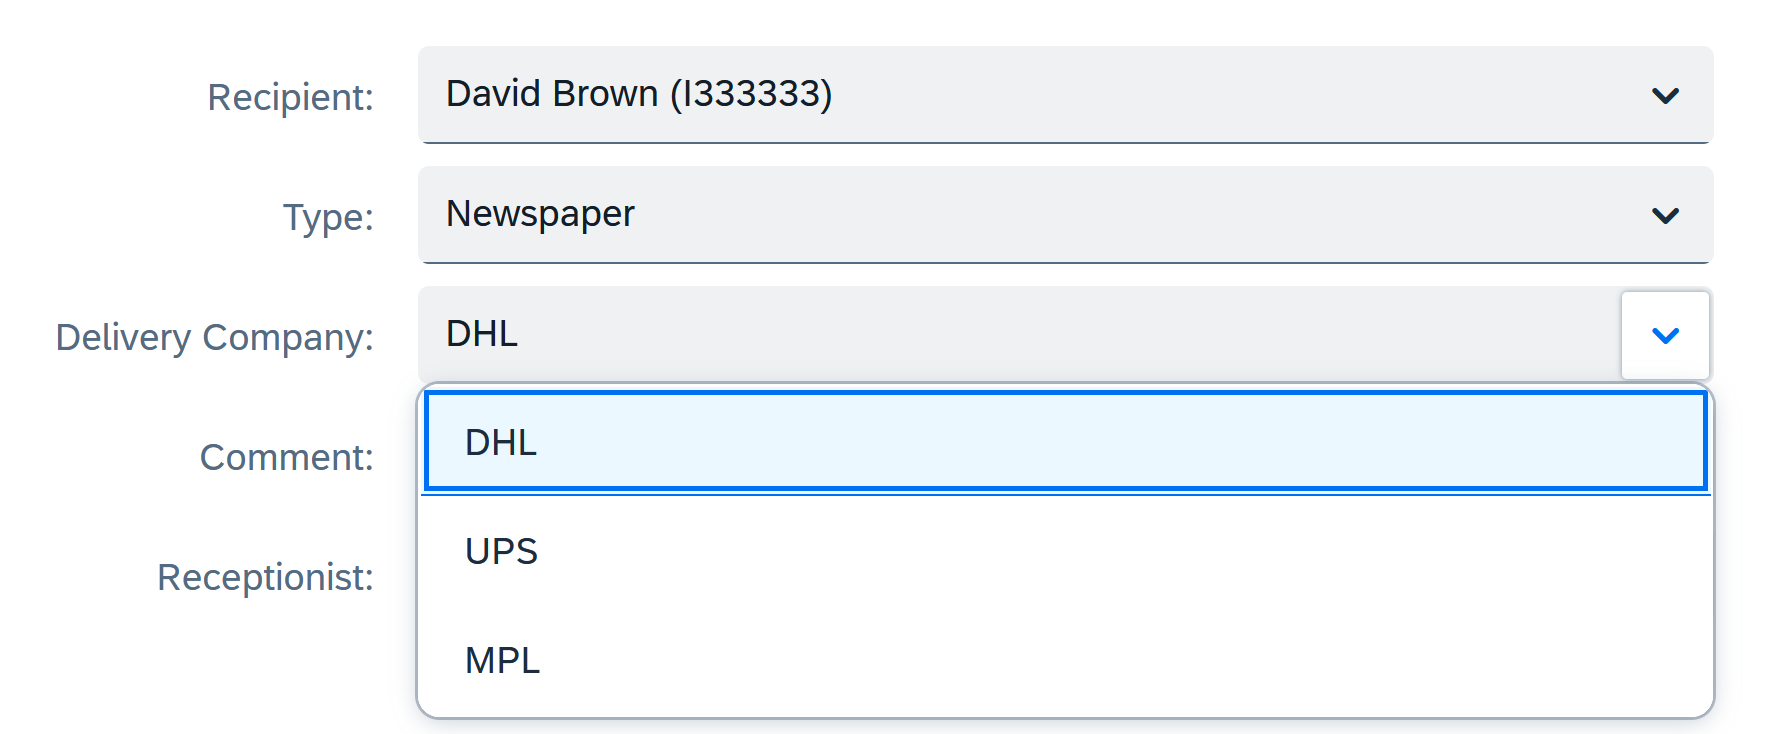
\includegraphics[width=0.45\linewidth]{images/user_doc/registration/entry3.png}}
    \hspace{5pt}
    \subcaptionbox{Step 4: Input any Comment if Needed}{
		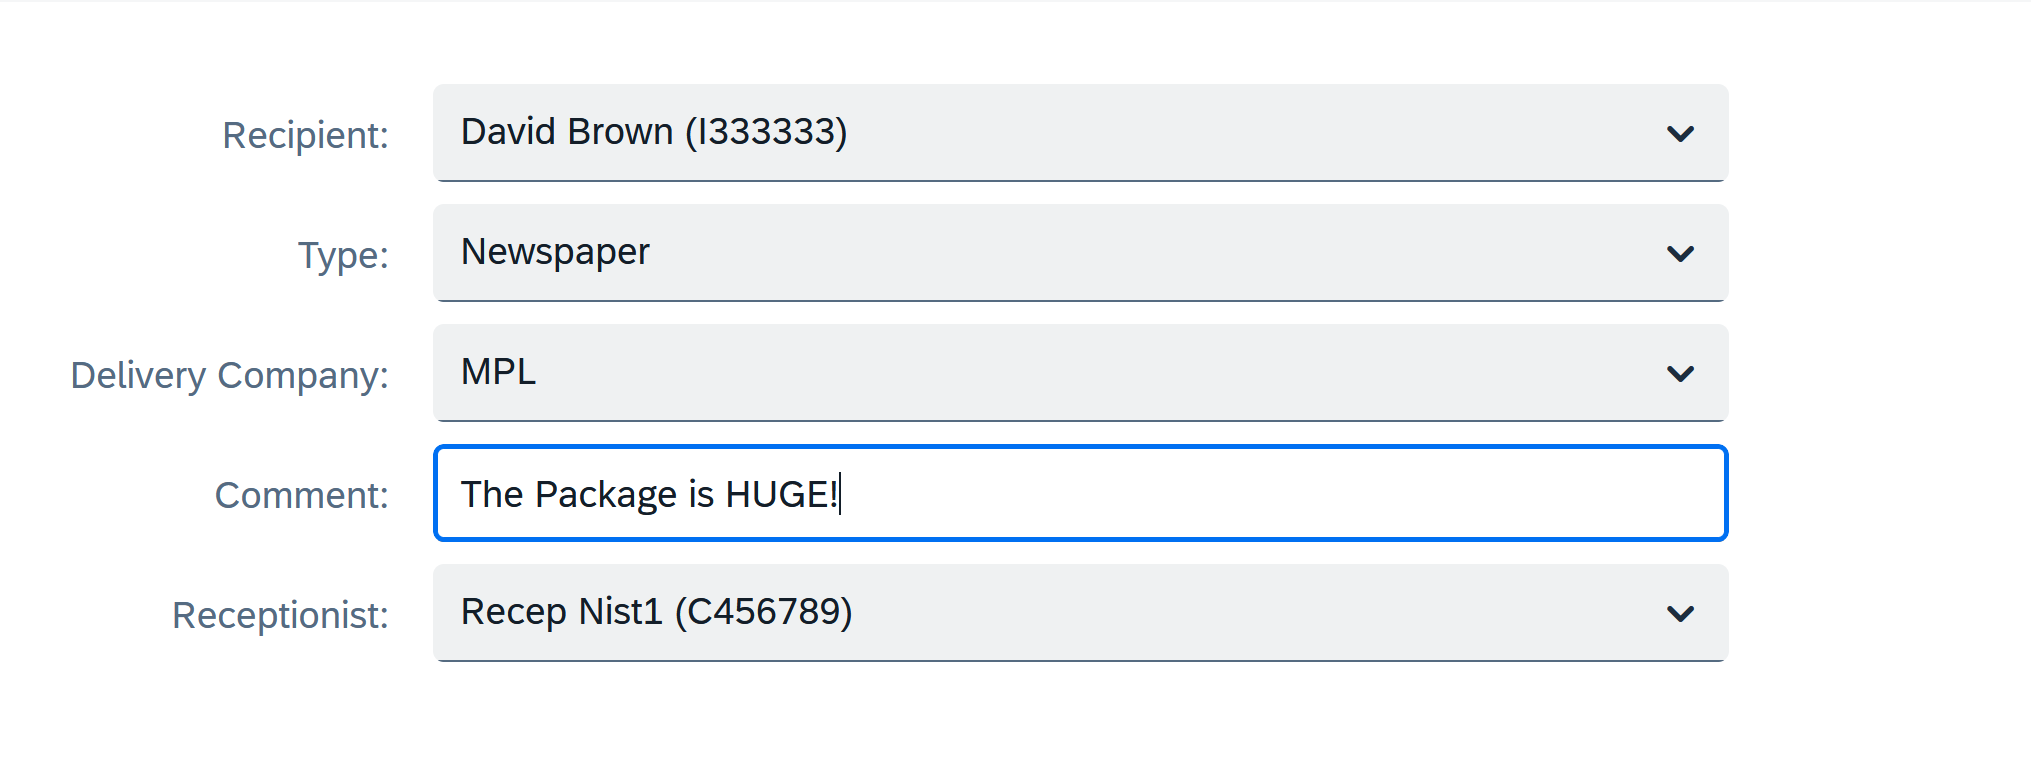
\includegraphics[width=0.45\linewidth]{images/user_doc/registration/entry4.png}}

    	\subcaptionbox{Step 3: Choose Responsible Receptionist}{
		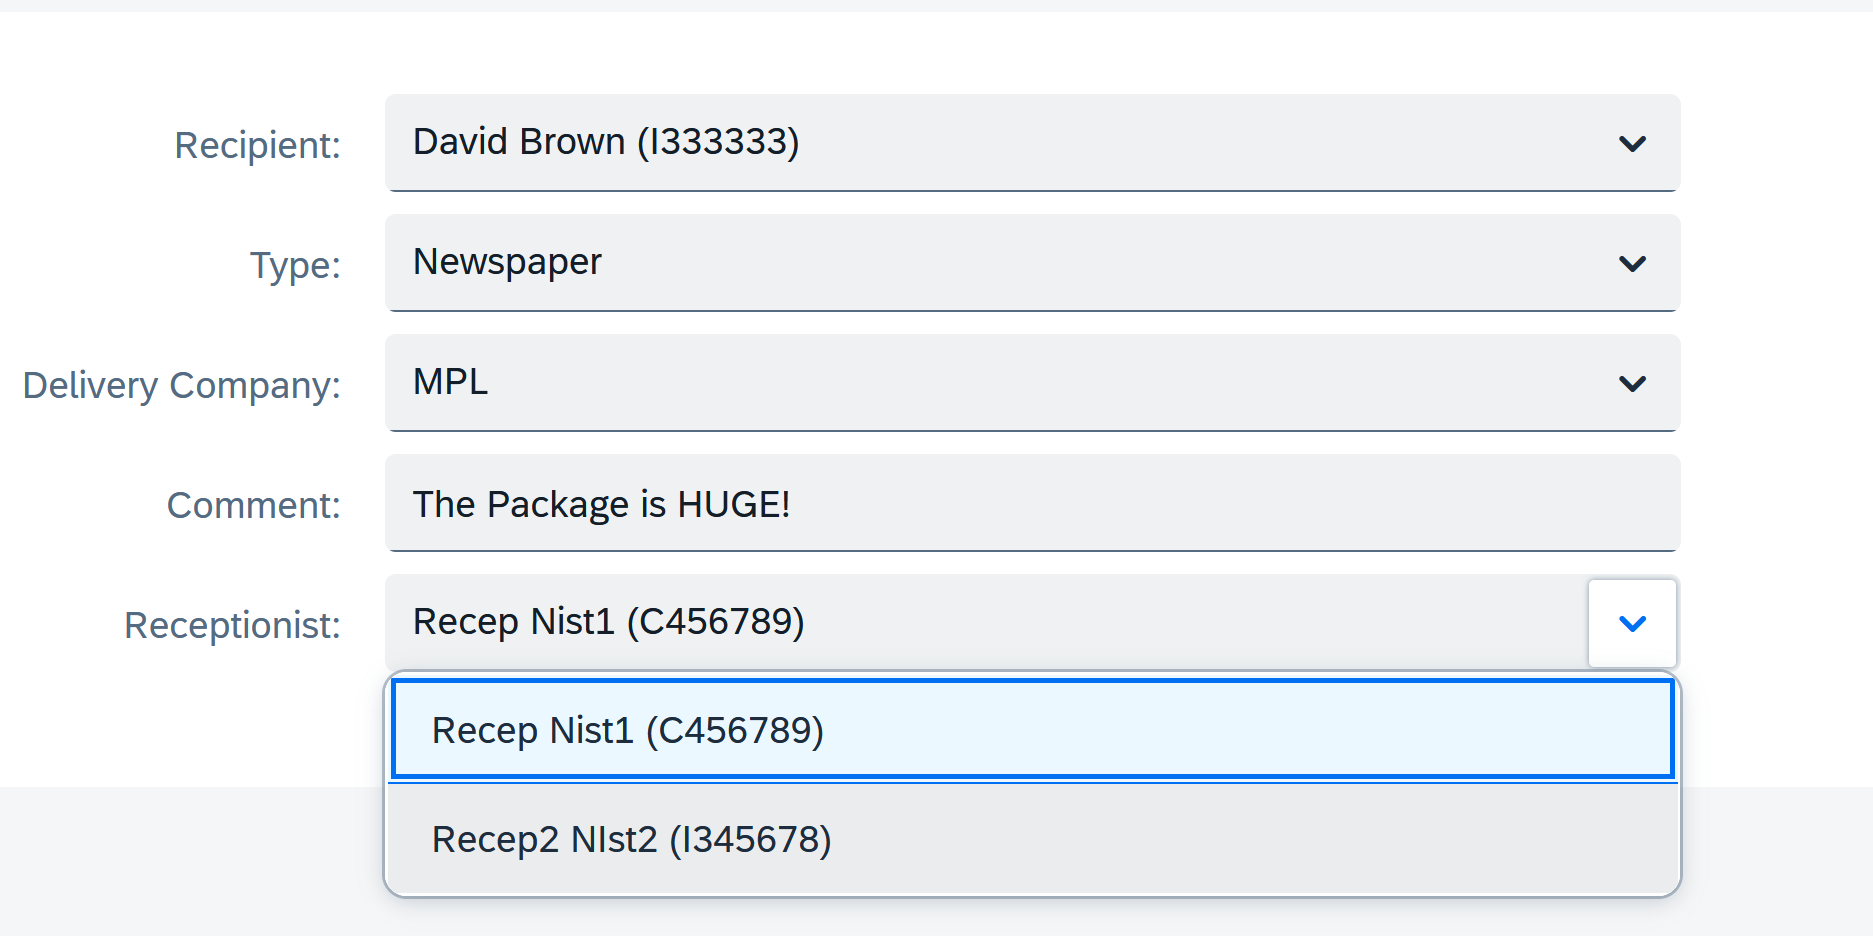
\includegraphics[width=0.45\linewidth]{images/user_doc/registration/entry5.png}}
  
    \caption{Register Packages Form - Form Entry Guide}
	\label{fig:RPformEntry}
\end{figure}

\subsubsection{Data Submitting}

When \textbf{Receptionist} finished entering the form and click the "Save" button, the entered package details are submitted, a package with \textit{new} status is created in the system, a success message toast appears and \textbf{Receptionist} is then navigated automatically to the \textbf{Manage Package} application. (\autoref{fig:RPsaveOp})

When \textbf{Receptionist} finished entering the form and click the "Save and New" button, the entered package details are submitted, a package with \textit{new} status is created in the system, a success message toast appears and the form is reset to default state. \textbf{Receptionist} may then start to register another package. (\autoref{fig:RPsaveNewOp})

When \textbf{Receptionist} finished entering the form and click the "Discard" button, the form is reset to default state and \textbf{Receptionist} is navigated back to the launch pad. (\autoref{fig:RPdiscardOp})

\begin{figure}[H]
	\centering
    \begin{subfigure}{1\linewidth}
        \centering
        \subcaptionbox {Success Toast}{
            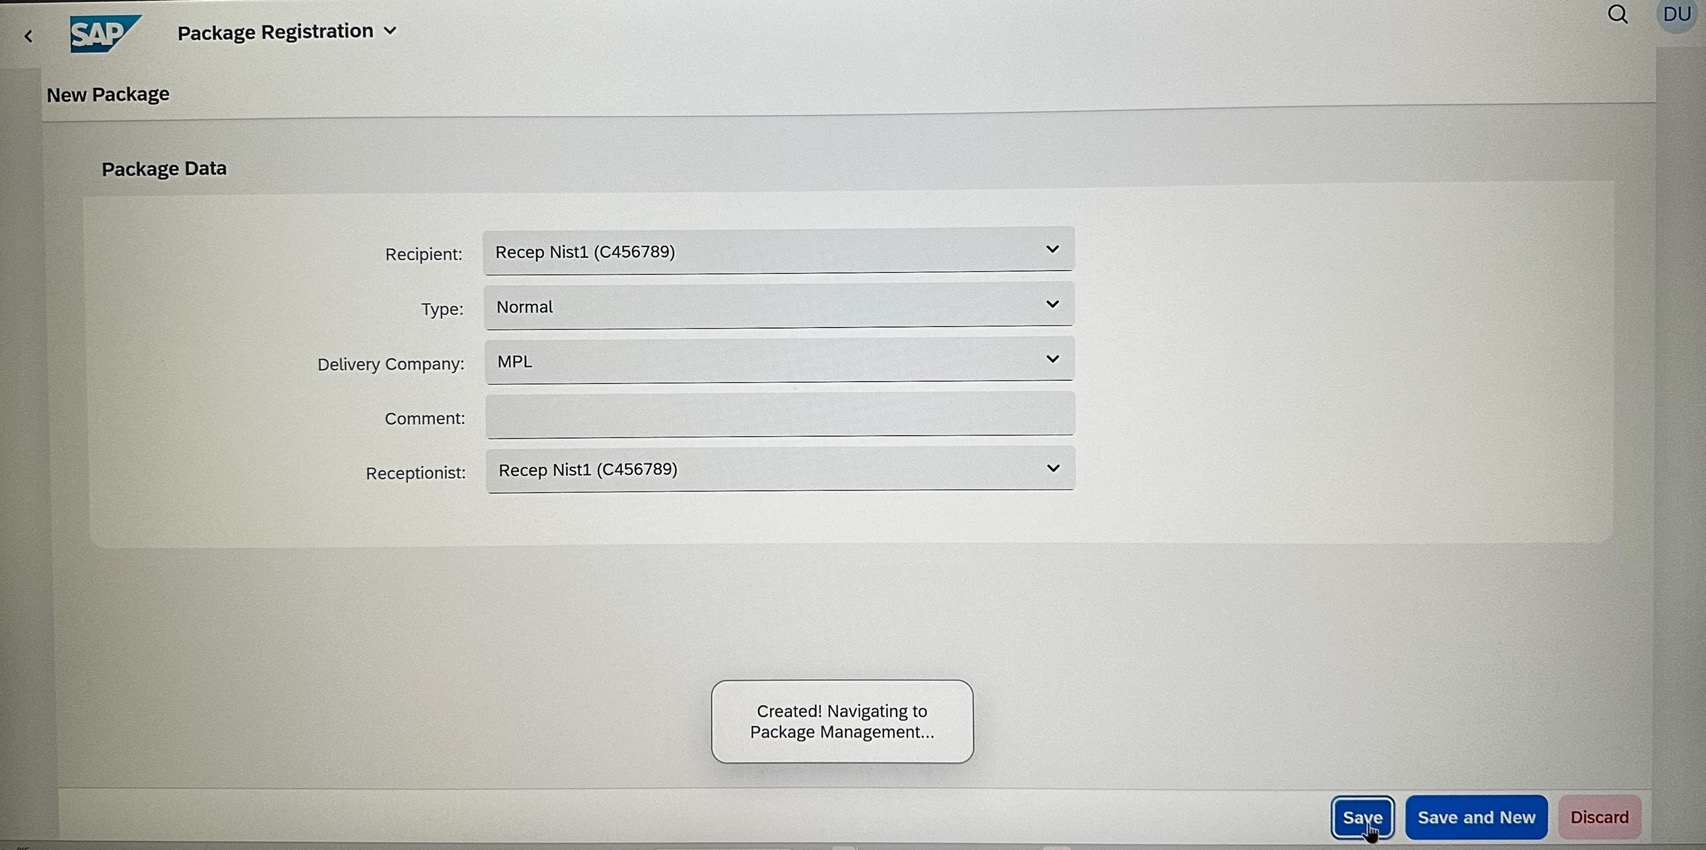
\includegraphics[width=0.45\linewidth]{images/user_doc/registration/SaveToast.jpg}
        }
        \vspace{5pt}
        \subcaptionbox {Target Navigation - Manage Package}{
            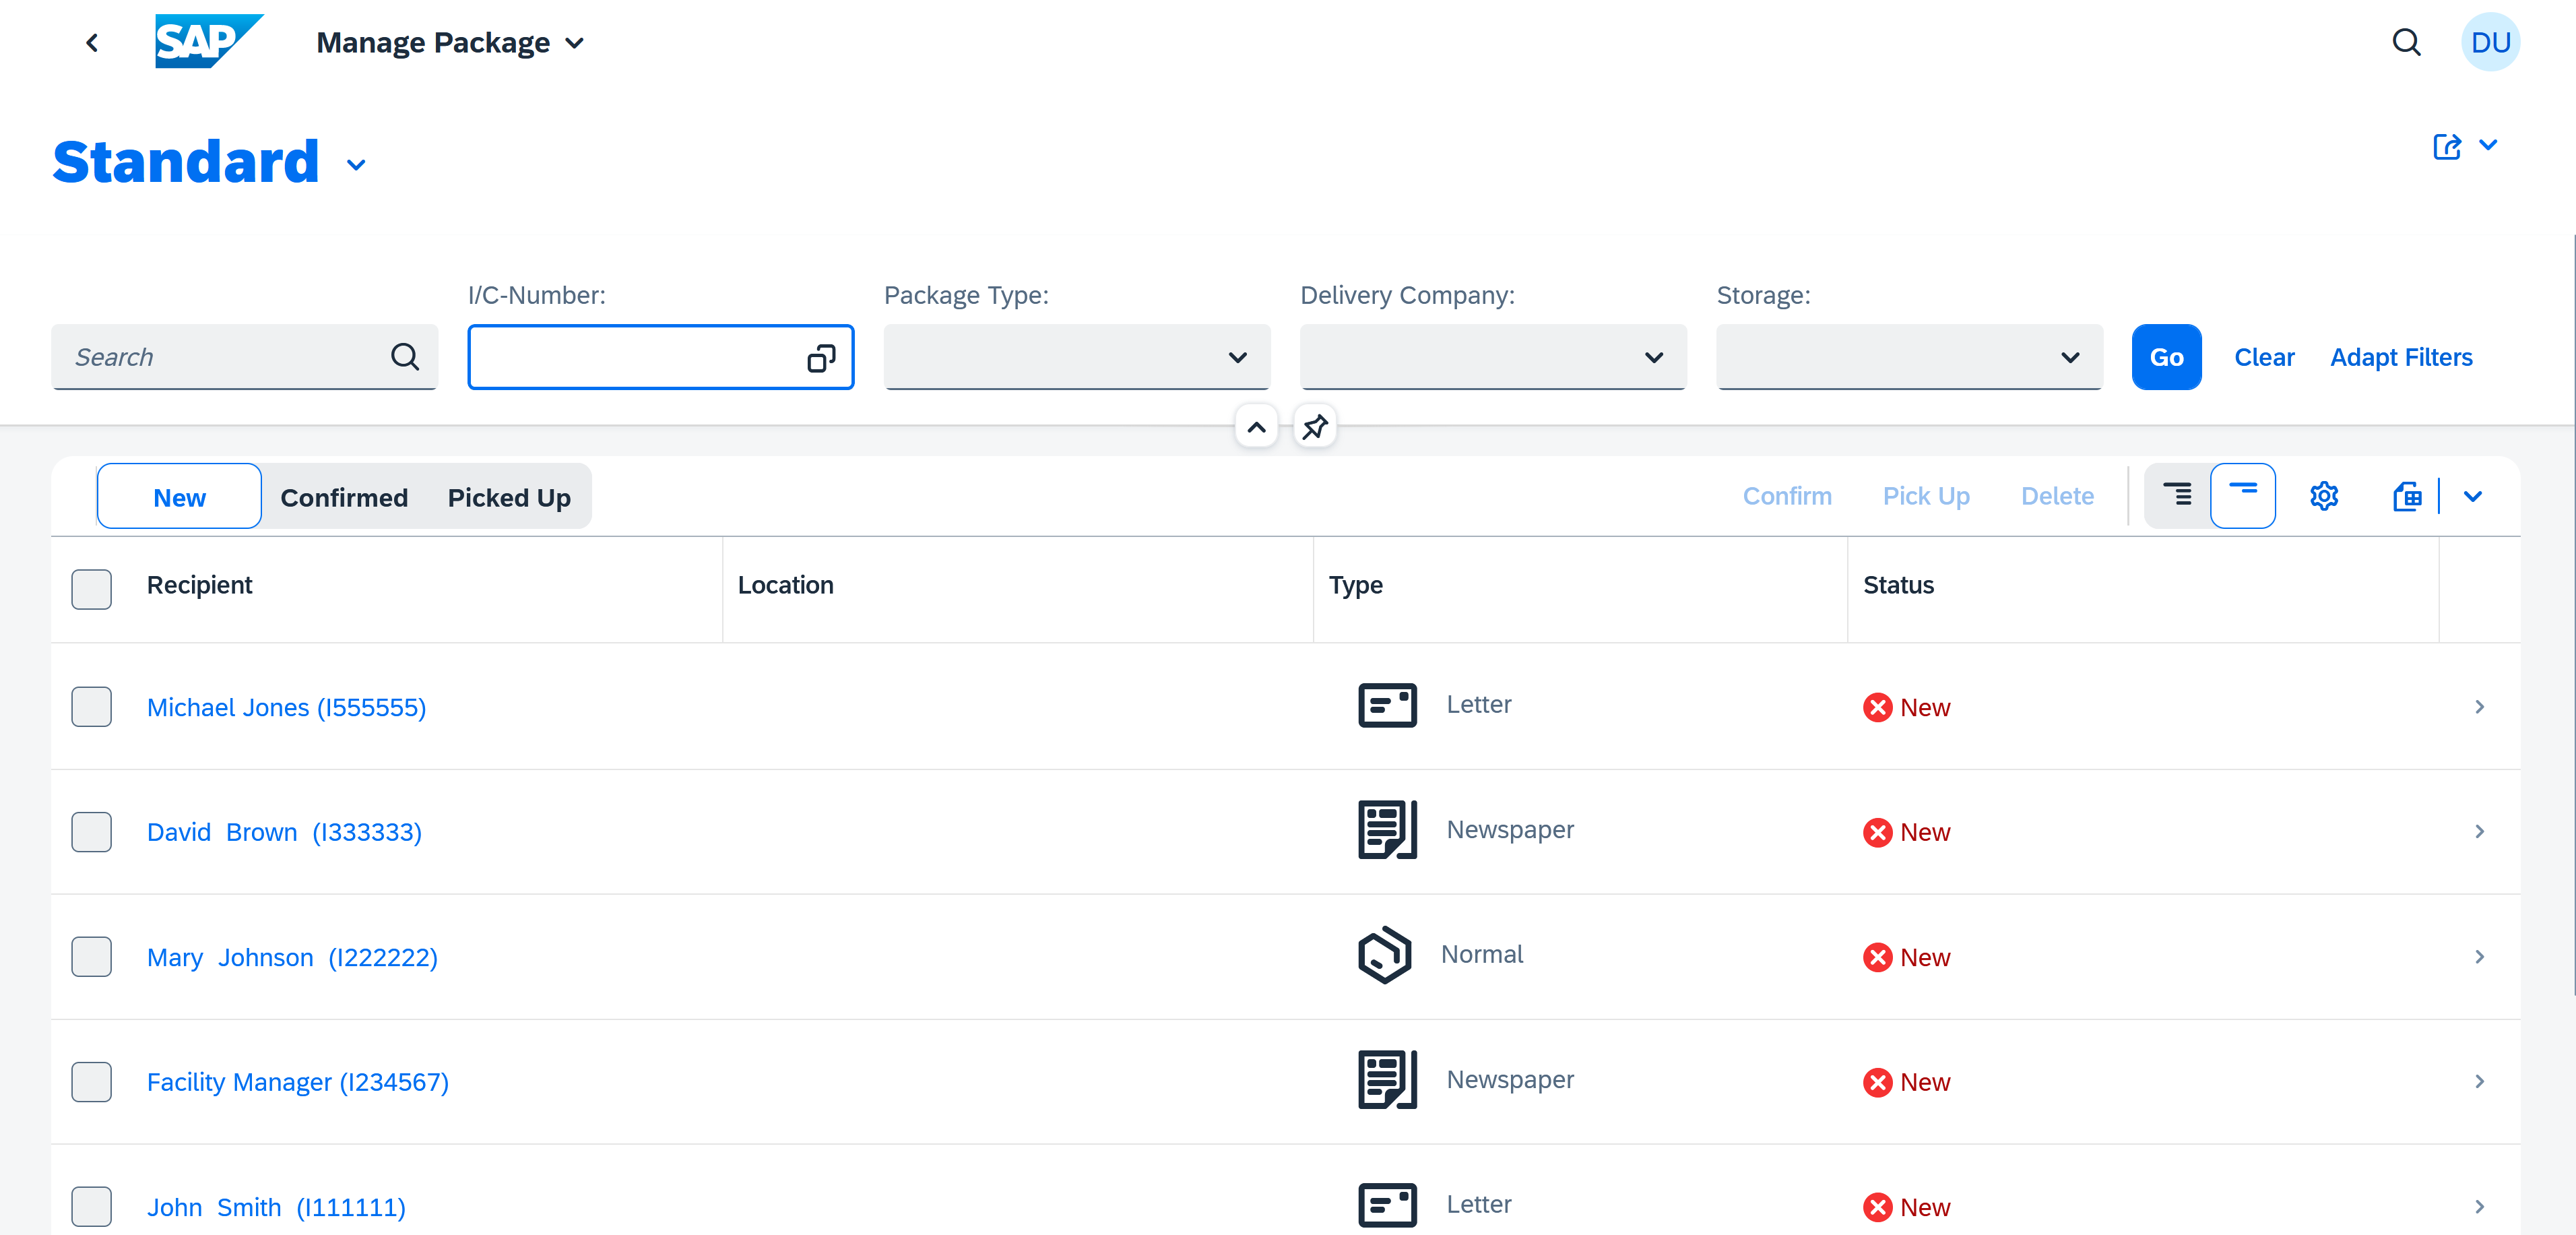
\includegraphics[width=0.45\linewidth]{images/user_doc/registration/target.png}
        }
        \caption{Option 1: Save}
    \end{subfigure}%
    \caption{Register Packages Form - Option 1: Save}
    \label{fig:RPsaveOp}
\end{figure}

\begin{figure}[H]
	\centering
    \begin{subfigure}{1\linewidth}
        \centering
        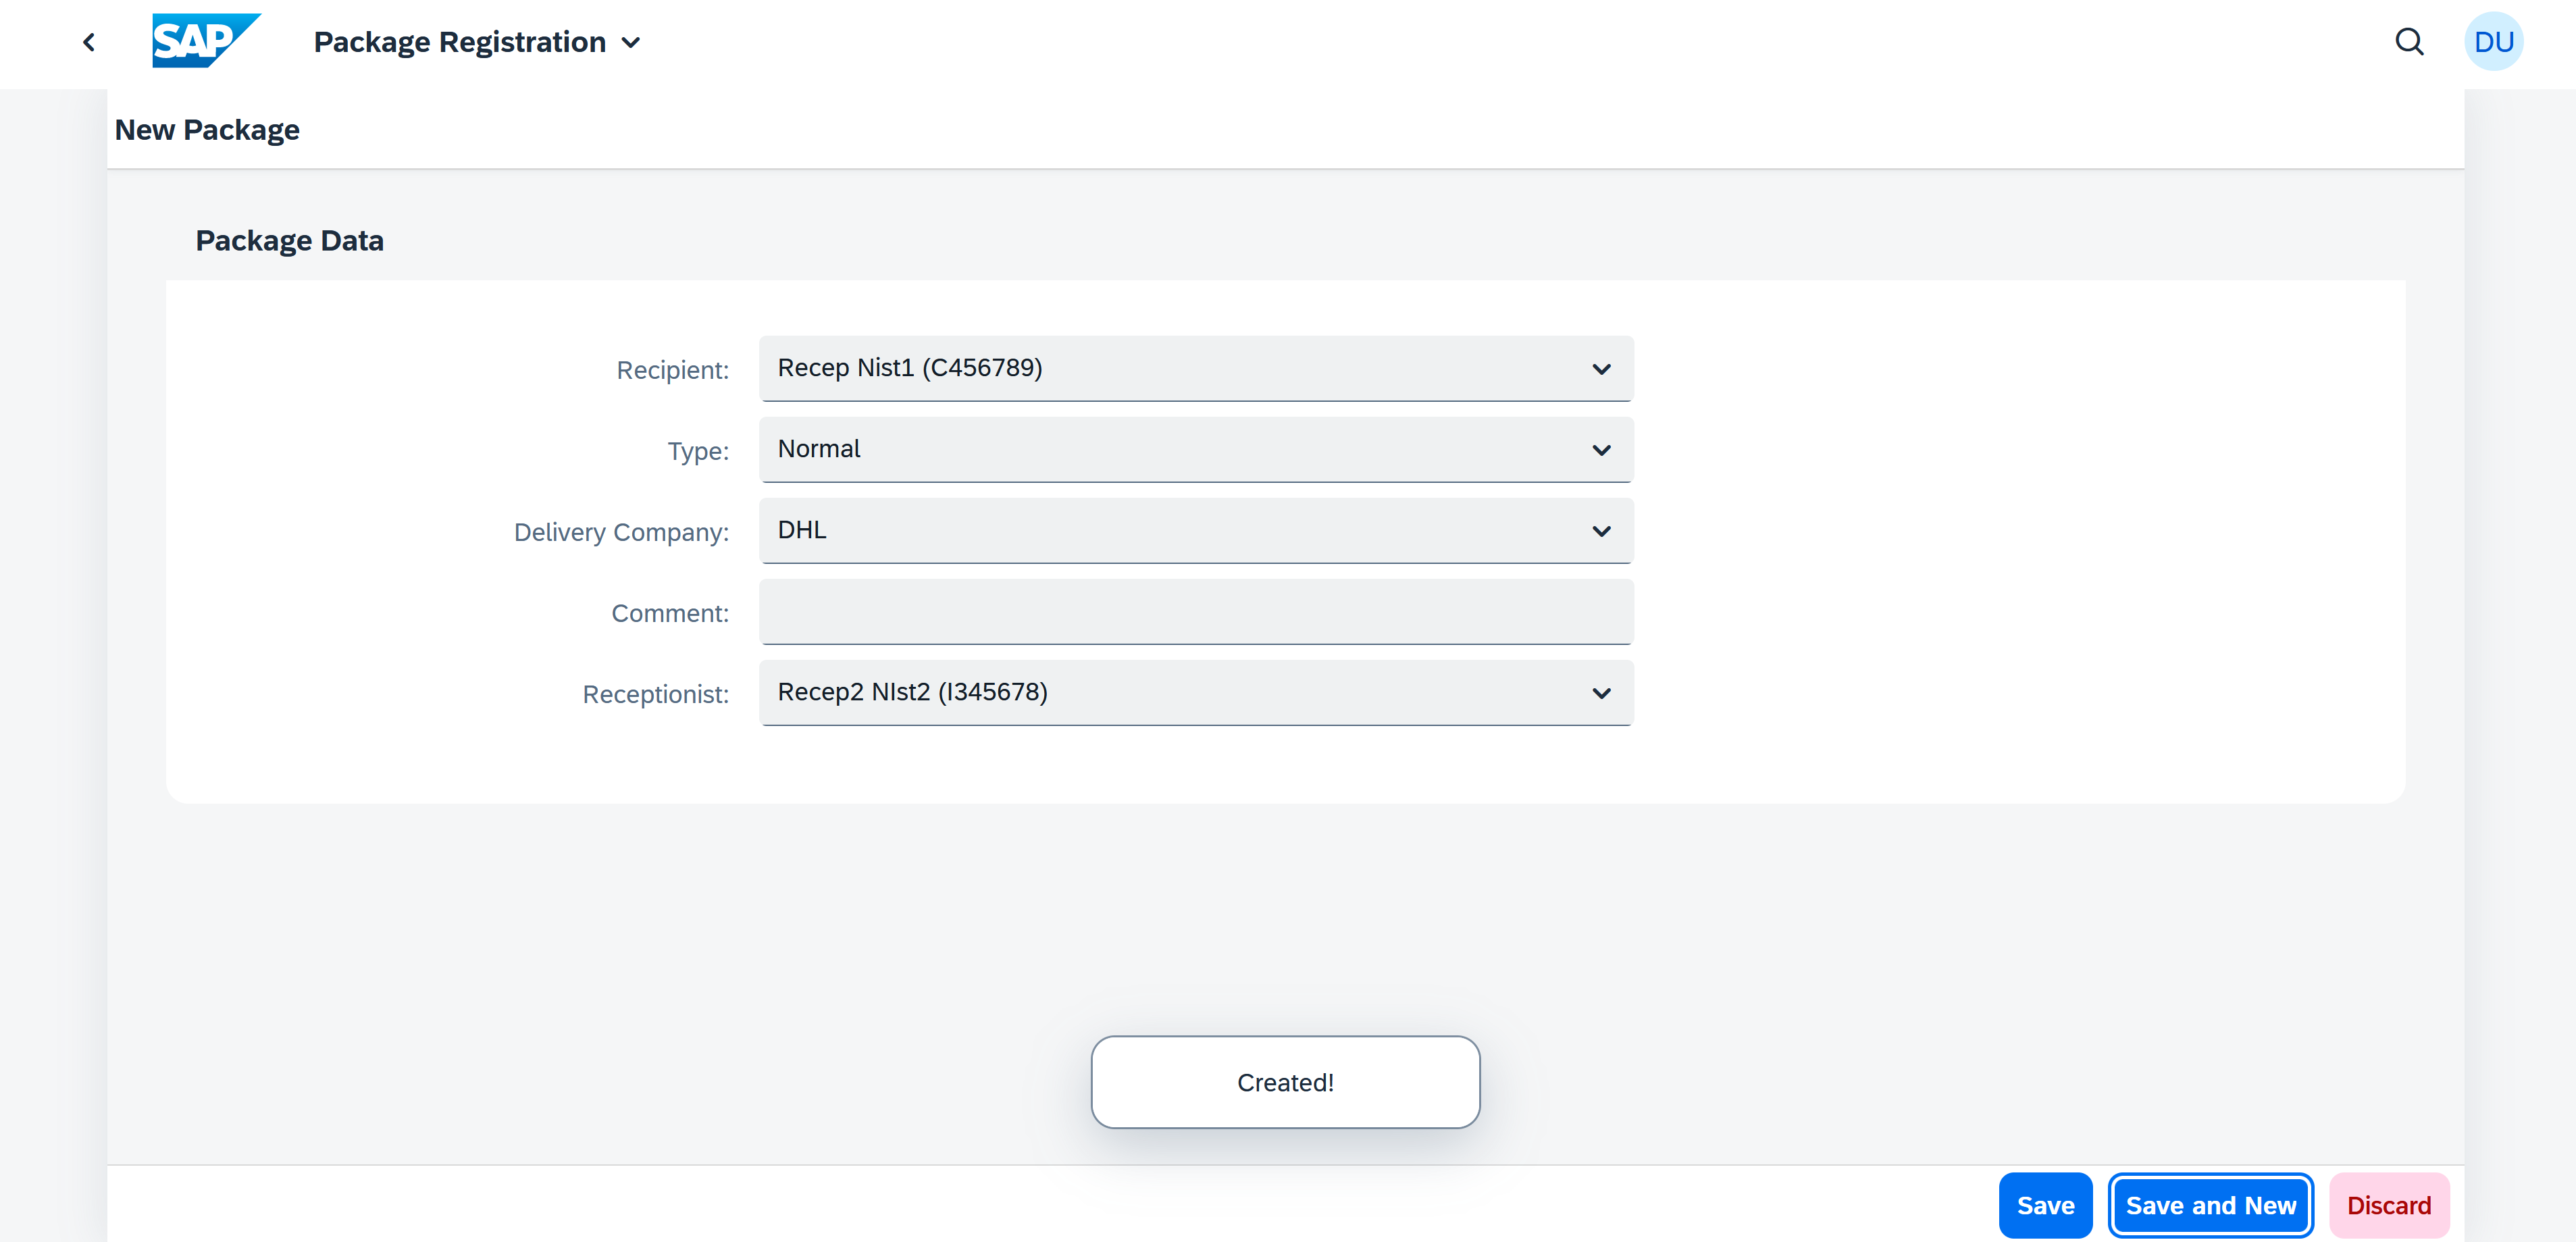
\includegraphics[width=1\linewidth]{images/user_doc/registration/saveAndNewToast.png}
    \end{subfigure}
    \caption{Register Packages Form - Option 2: Save and New}
    \label{fig:RPsaveNewOp}
\end{figure}

\begin{figure}[H]
	\centering
    \begin{subfigure}{1\linewidth}
        \centering
        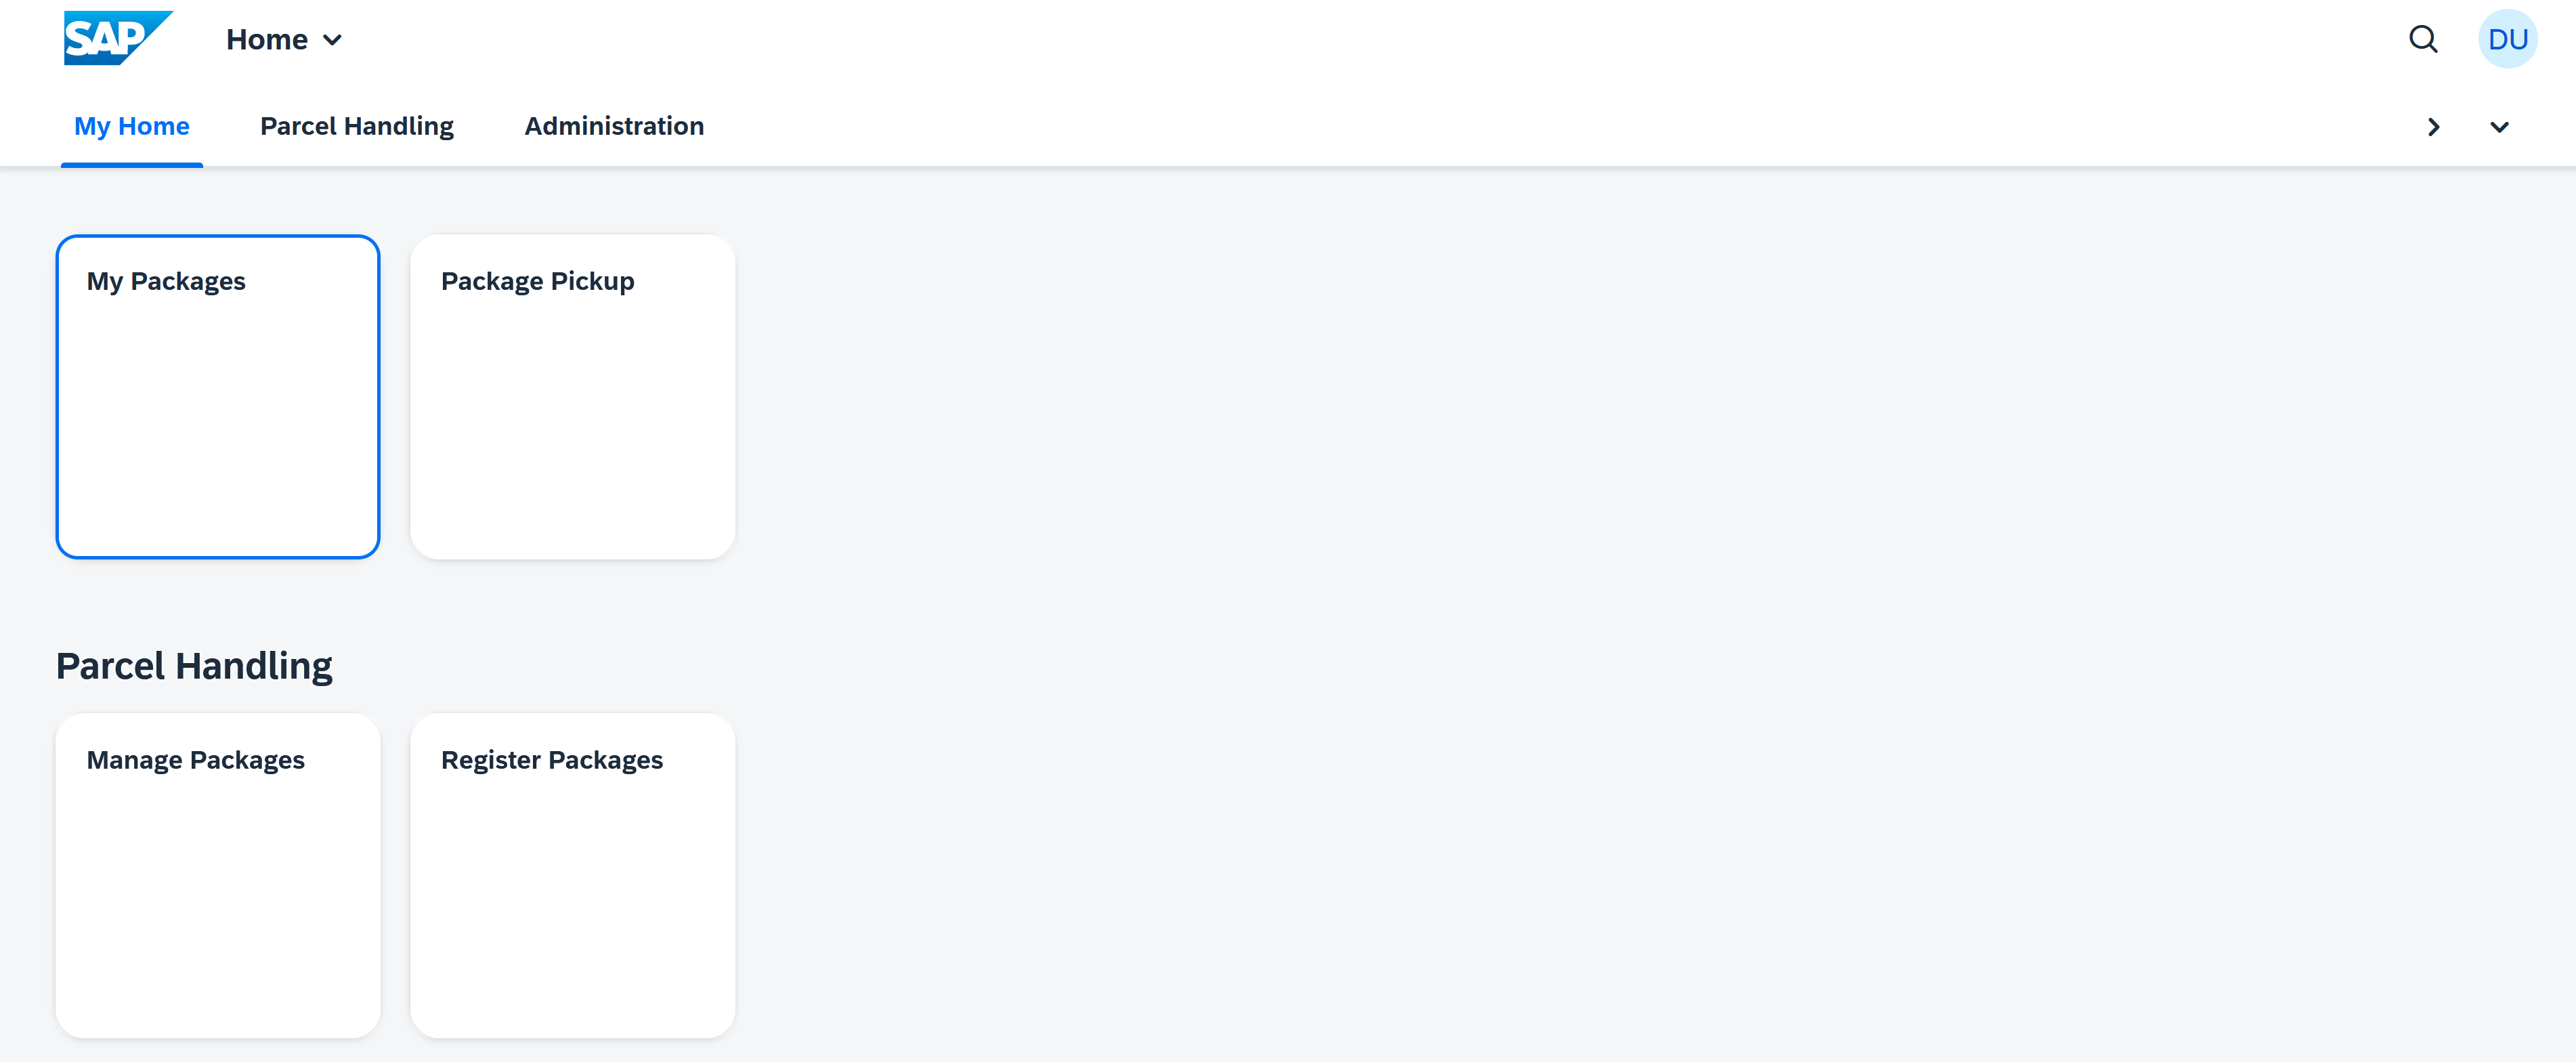
\includegraphics[width=1\linewidth]{images/user_doc/registration/discardTarget.png}
    \end{subfigure}
    \caption{Register Packages Form - Option 3: Discard}
    \label{fig:RPdiscardOp}
\end{figure}

\subsection{Manage Packages}                     
\label{subsec:mp}

The \textbf{Manage Packages} application is designed for \textbf{Receptionist} (See \autoref{sec:UdocReceptionist} for all receptionist related applications) to edit, confirm, pickup, check the existing packages in the system. The summarized main actions a \textbf{Receptionist} can take are listed here:

\begin{compactenum}
	\item Browse the existing packages.
        \begin{compactenum}
            \item Filtering possibility.
            \item Quick variant switch based on package status.
            \item Report List of packages info with selection capability.
            \item Detail page for single packages.
        \end{compactenum}
    \item Confirm package(s) which status is new.
    \item Pickup a package (single at a time) which status is confirmed. (As a backup manuvor in case the employee cannot access to mobile devices.
    \item Delete package(s) which status is new or confirmed.
    \item Edit package(s)' recipient, type, delivery company, and comment.
\end{compactenum}

\bigskip
Further explanation and restrictions of these operations are detailed in the coming sections.

\begin{figure}[H]
	\centering
	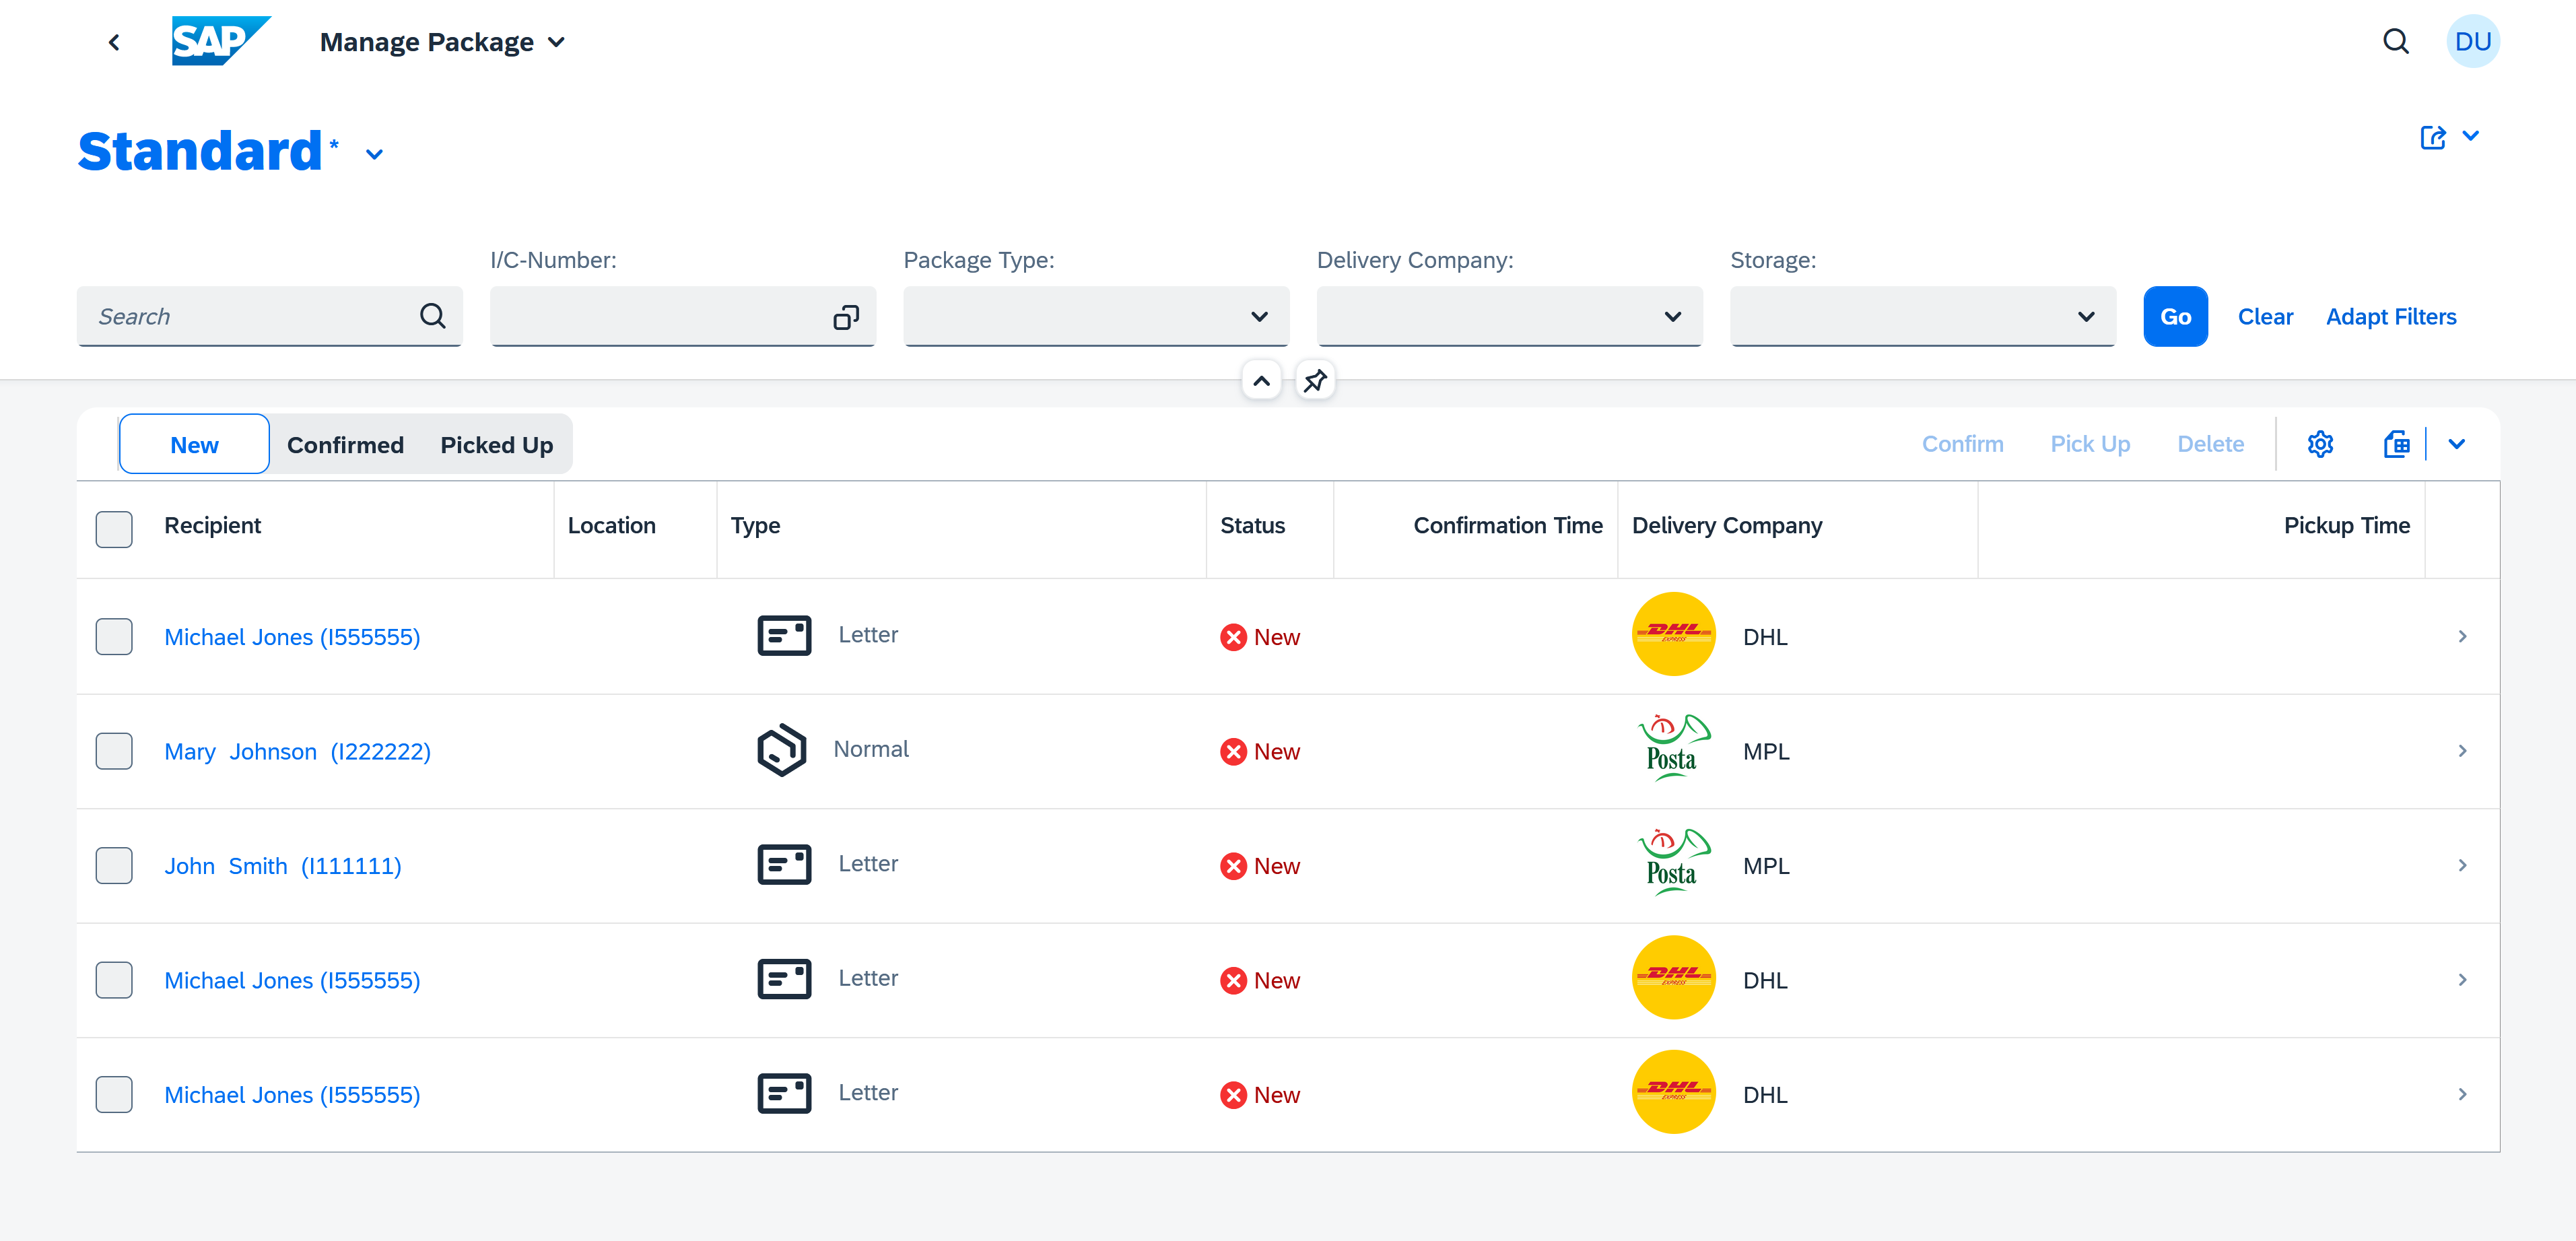
\includegraphics[height=200pt]{images/user_doc/managePack/ReportScreen/browse/Overview.png}
	\caption{Manage Packages Report Screen - Overview}
	\label{fig:MPReportOverview}
\end{figure}


\subsubsection{Browse Packages}
As an \textbf{Receptionist}, after clicking at the application tile, is redirected to the "Report Screen", which is the main screen of this application (\autoref{fig:MPReportOverview}). 
The upper part displays the search bar and the possible filters (\autoref{fig:MPFIlterBar}). 
In case the need of free text search of any possible content of the column, one can use the \textbf{"Search Bar"}. (\autoref{fig:MPSearchBar}) The search supports in-completed keywords and is case insensitive. One can also use the predefined filters, where value helps and entry helps are provided.
The default predefined filters are: \textbf{I/C-Number} (free text SAP ID input, \autoref{fig:MPIDFIlter}), \textbf{Type} (drop down of all available types), \textbf{Delivery Company} (drop down of all available companies) and \textbf{Storage} (drop down of all available storage). 
For drop down filters, one can click at the small drop down arrow and select zero to many options (\autoref{fig:MPDefaultDropDown}). When adjusting the filtering values, the list view is temporarily locked. After adjusting the filtering values, one can run and review the filter result by clicking the "Go" Button. (\autoref{fig:MPAjustFilters})

\begin{figure}[H]
	\centering
	
\includegraphics[width=1\linewidth]{images/user_doc/managePack/ReportScreen/browse/FilterBar.png}
	\caption{Manage Packages Report Screen - Filter Bar}
	\label{fig:MPFIlterBar}
\end{figure}

\begin{figure}[H]
	\centering
	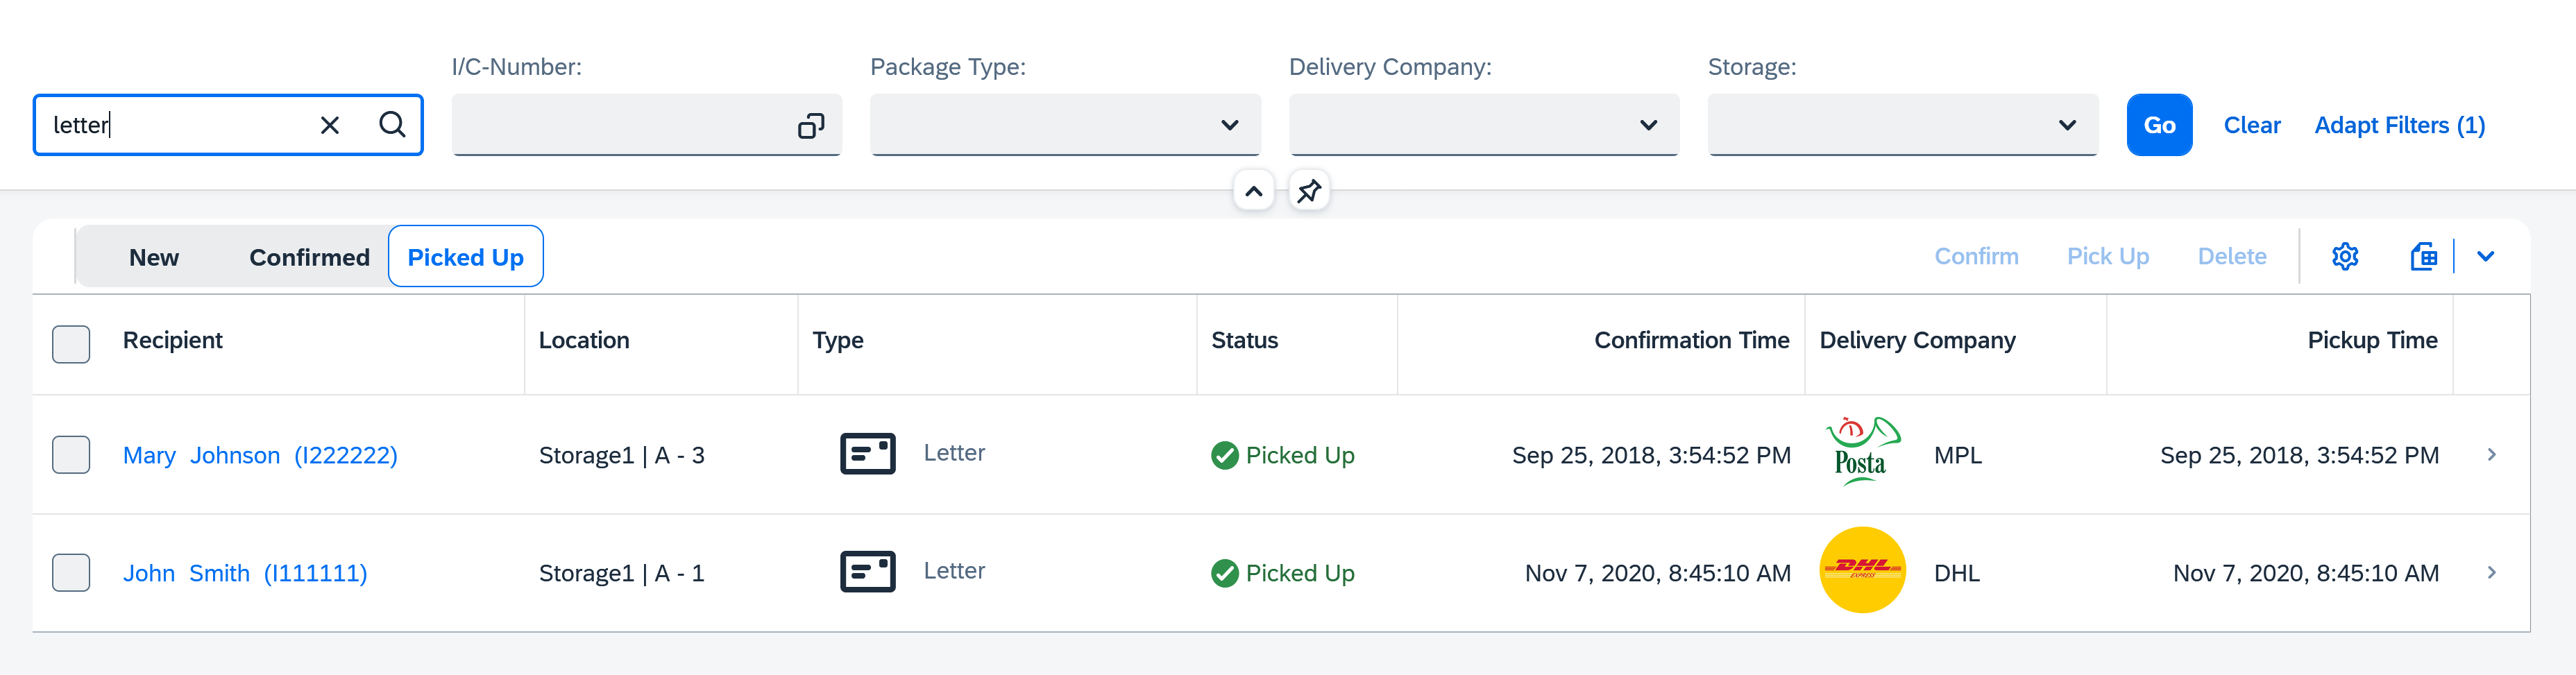
\includegraphics[width=1\linewidth]{images/user_doc/managePack/ReportScreen/browse/defaultSearchBarUsage.png}
	\caption{Manage Packages Report Screen - Filter Bar - Search Bar Usage Guide}
	\label{fig:MPSearchBar}
\end{figure}

\begin{figure}[H]
	\centering
	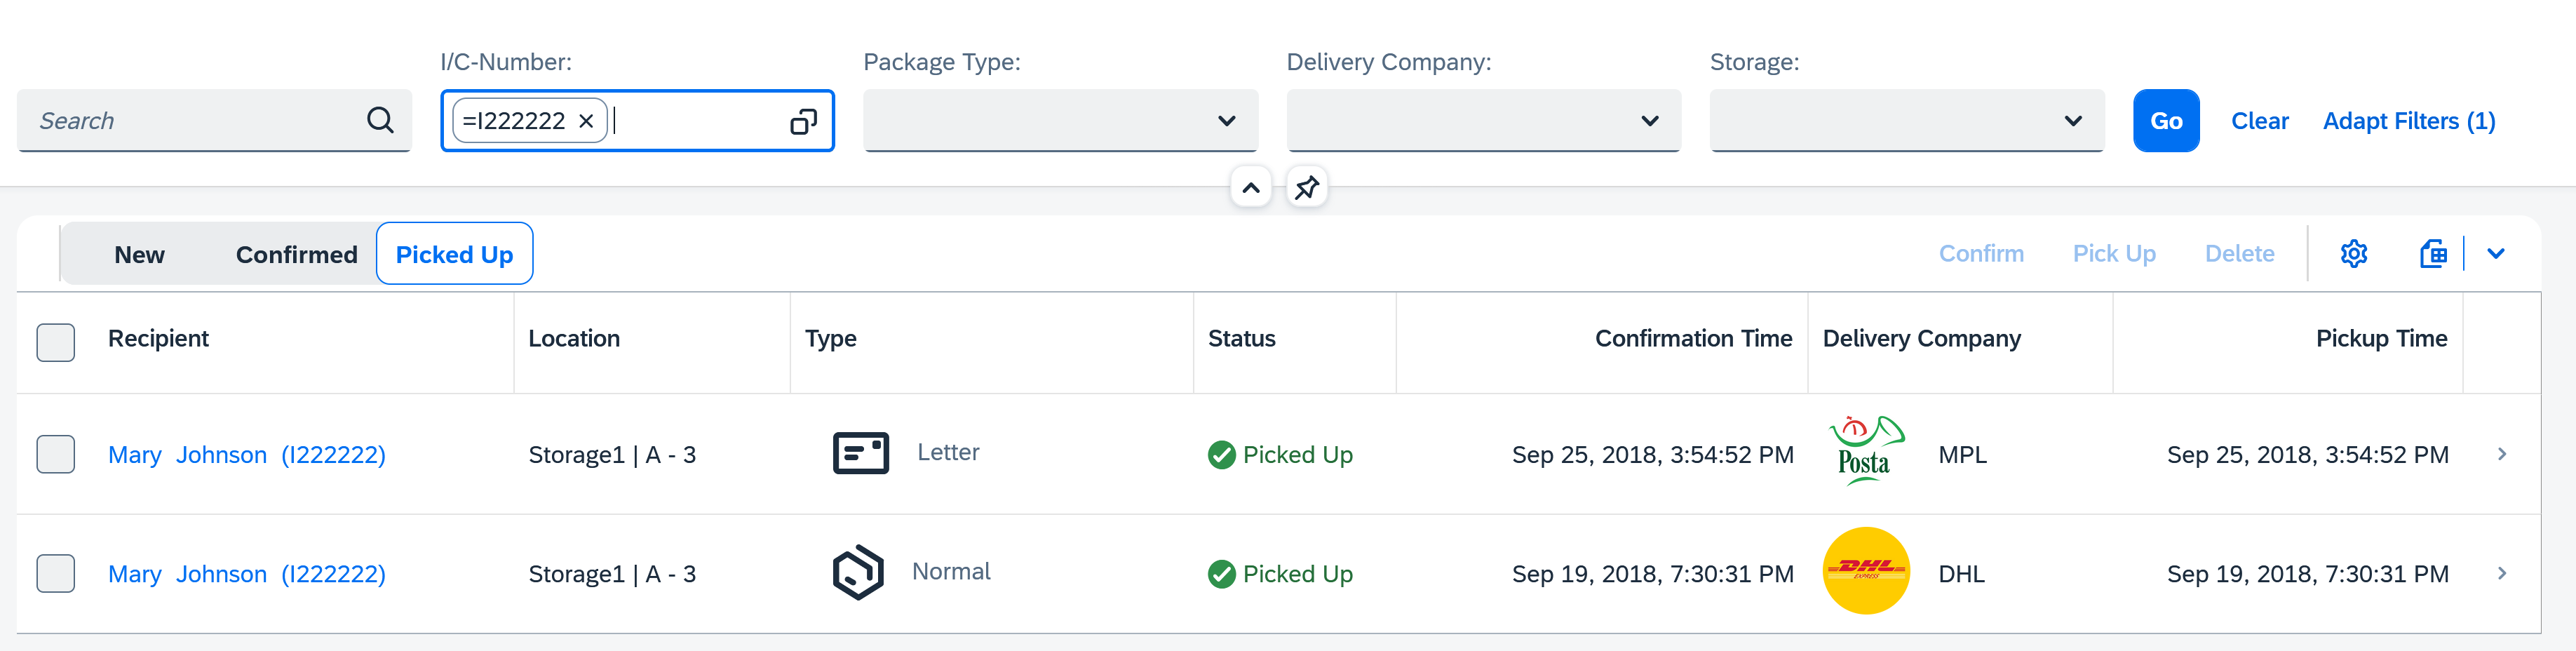
\includegraphics[width=1\linewidth]{images/user_doc/managePack/ReportScreen/browse/defaultFreeTextIdUsage.png}
	\caption{Manage Packages Report Screen - Filter Bar - ID Filter Usage Guide}
	\label{fig:MPIDFIlter}
\end{figure}

\begin{figure}[H]
	\centering
	\subcaptionbox{Type Filter}{
		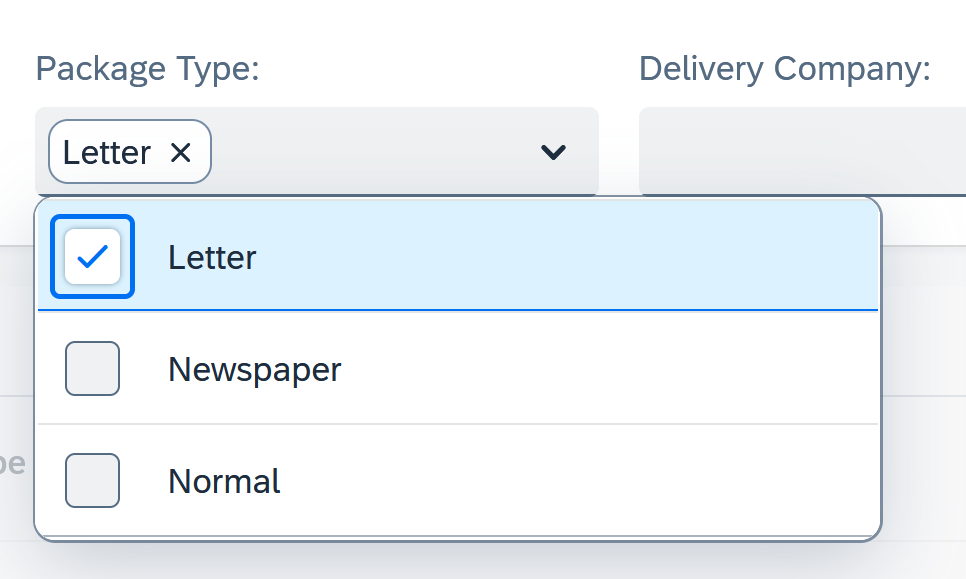
\includegraphics[width=0.45\linewidth]{images/user_doc/managePack/ReportScreen/browse/defaultType.png}}
	\hspace{5pt}
	\subcaptionbox{Company Filter}{
		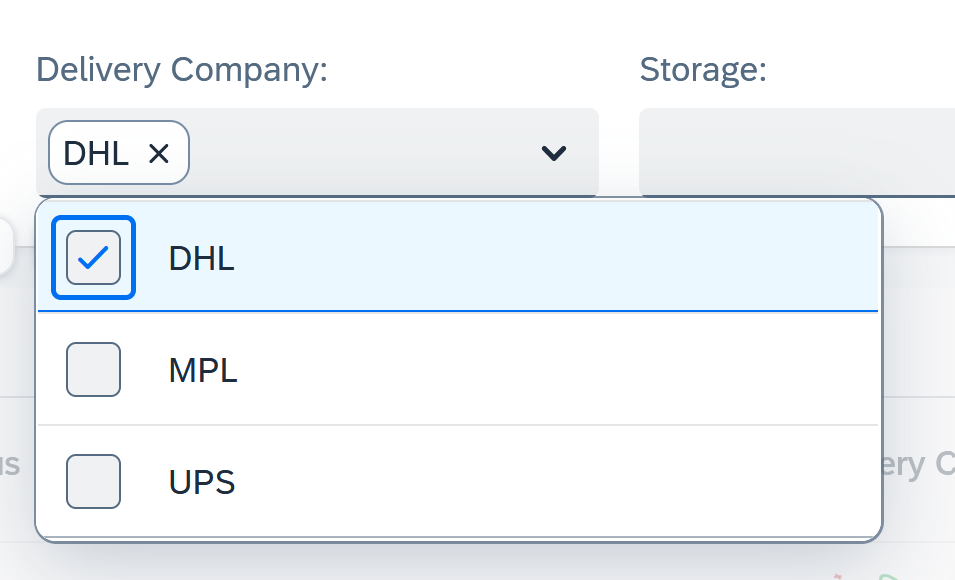
\includegraphics[width=0.45\linewidth]{images/user_doc/managePack/ReportScreen/browse/defaultCompany.png}}

    \subcaptionbox{Storage Filter}{
		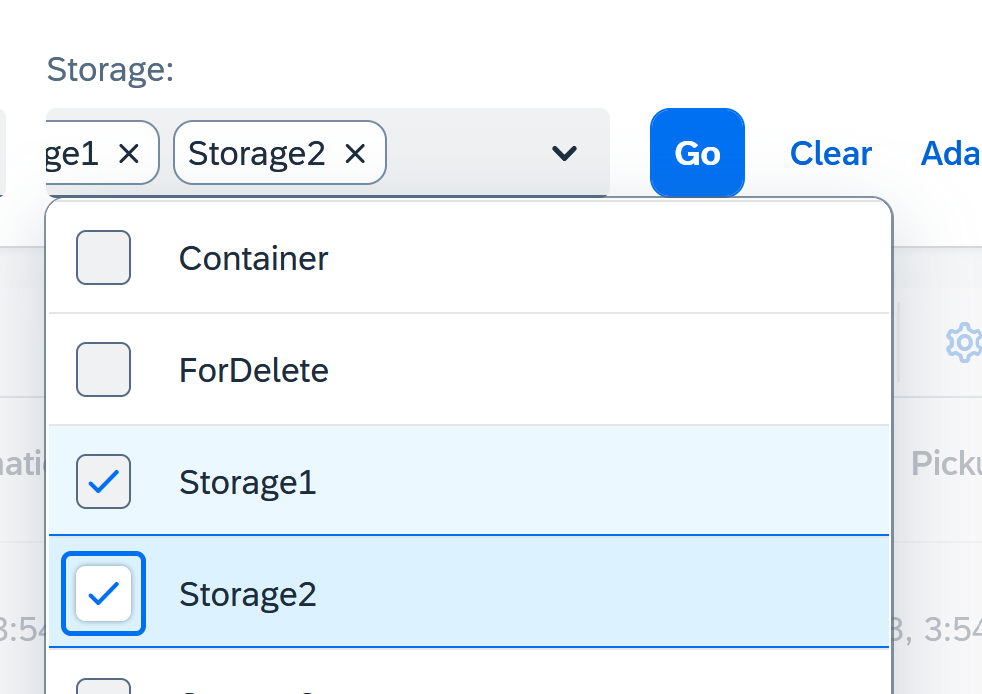
\includegraphics[width=0.45\linewidth]{images/user_doc/managePack/ReportScreen/browse/defaultStorage.png}}
	\caption{Manage Packages Report Screen - Filter Bar - Default Drop Down Filters Show Case}
	\label{fig:MPDefaultDropDown}
\end{figure}

\begin{figure}[H]
		\centering
	\subcaptionbox{While Adjusting the Filter}{
		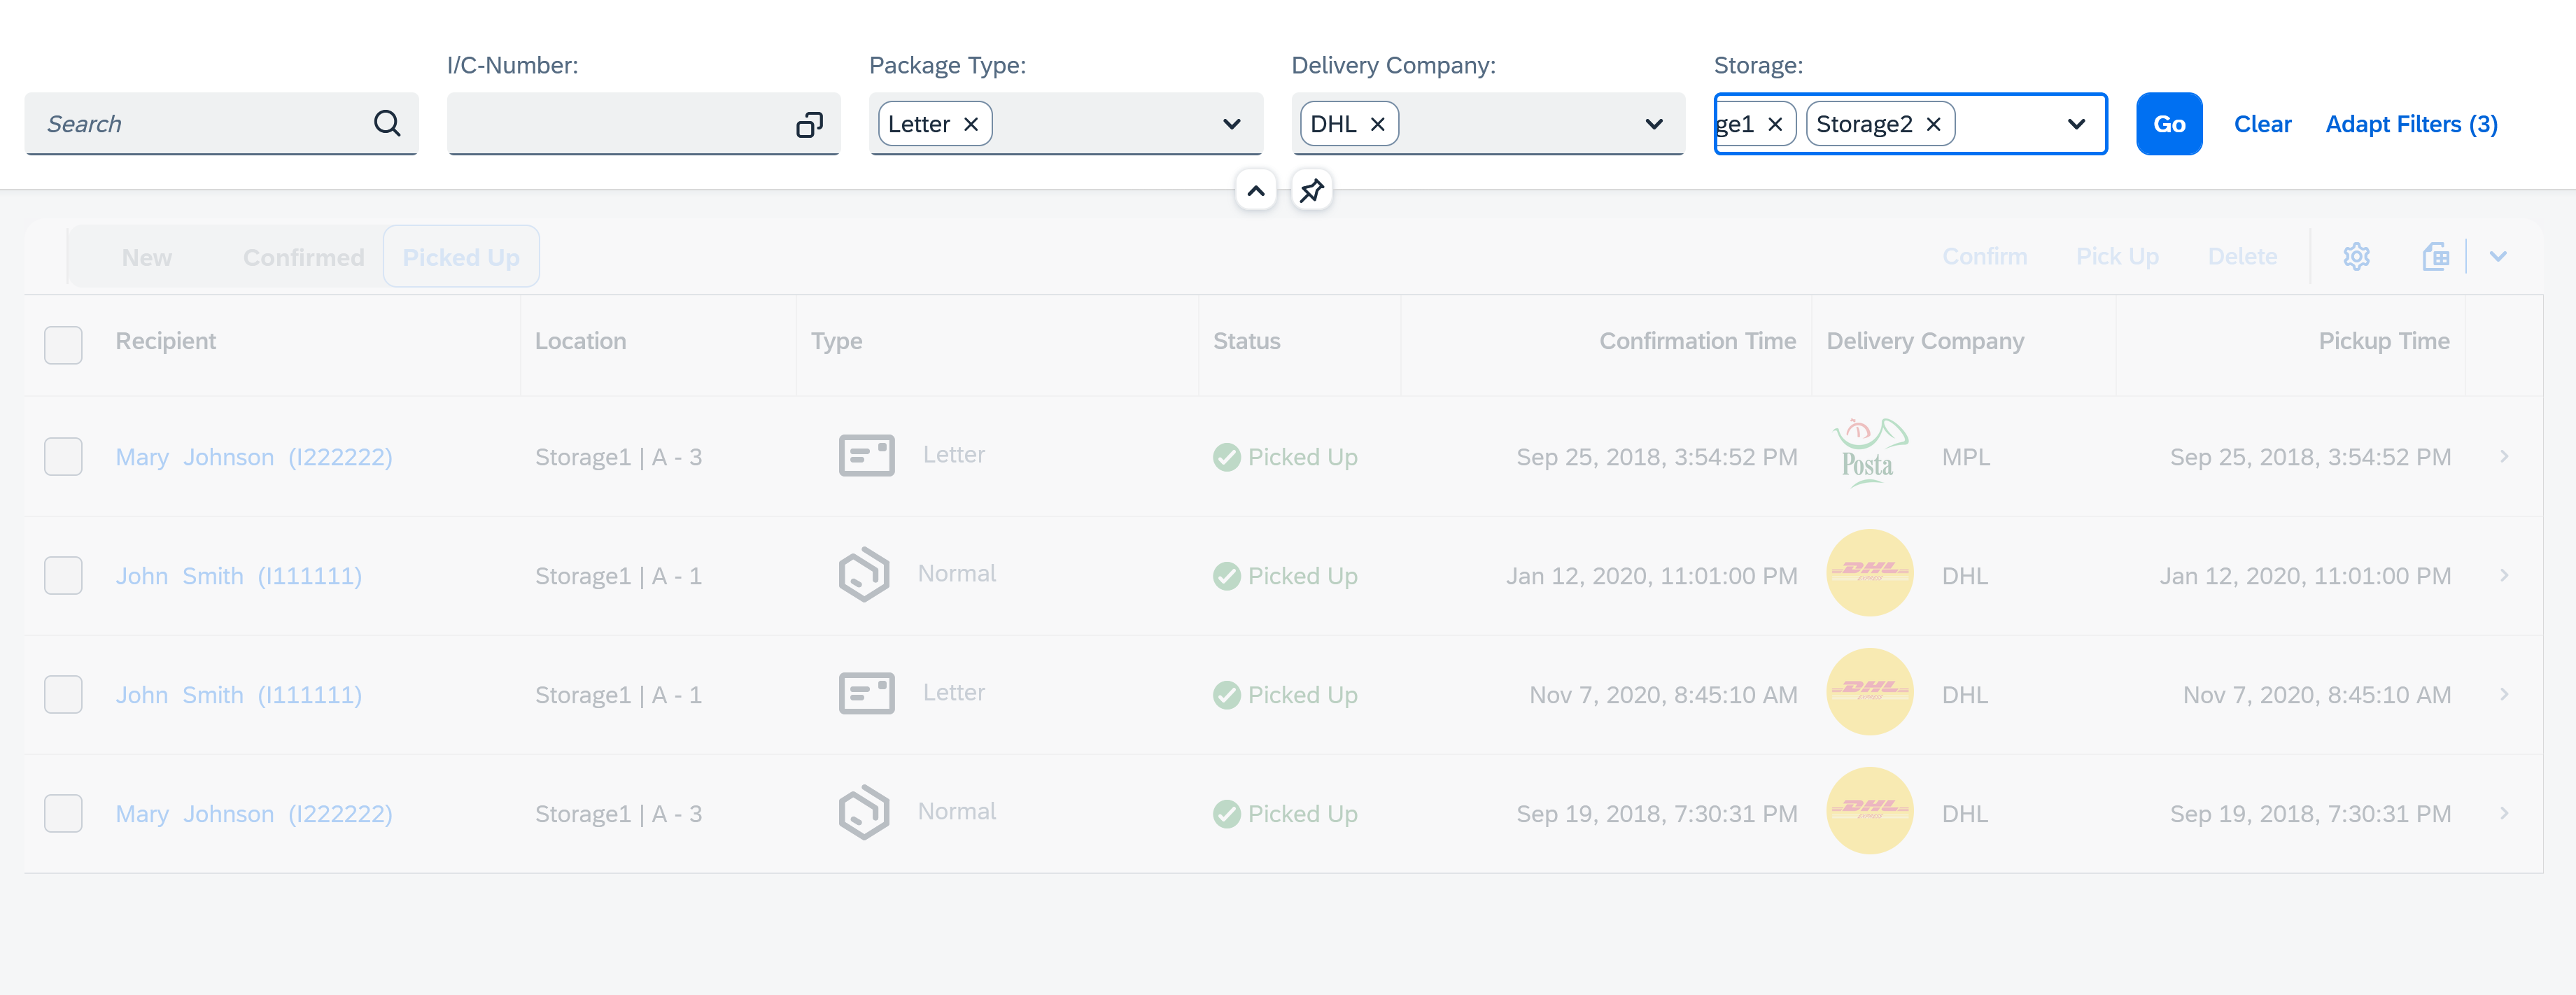
\includegraphics[width=0.45\linewidth]{images/user_doc/managePack/ReportScreen/browse/filterOnAdjusting.png}}
	\hspace{5pt}
	\subcaptionbox{Clicked "Go"}{
		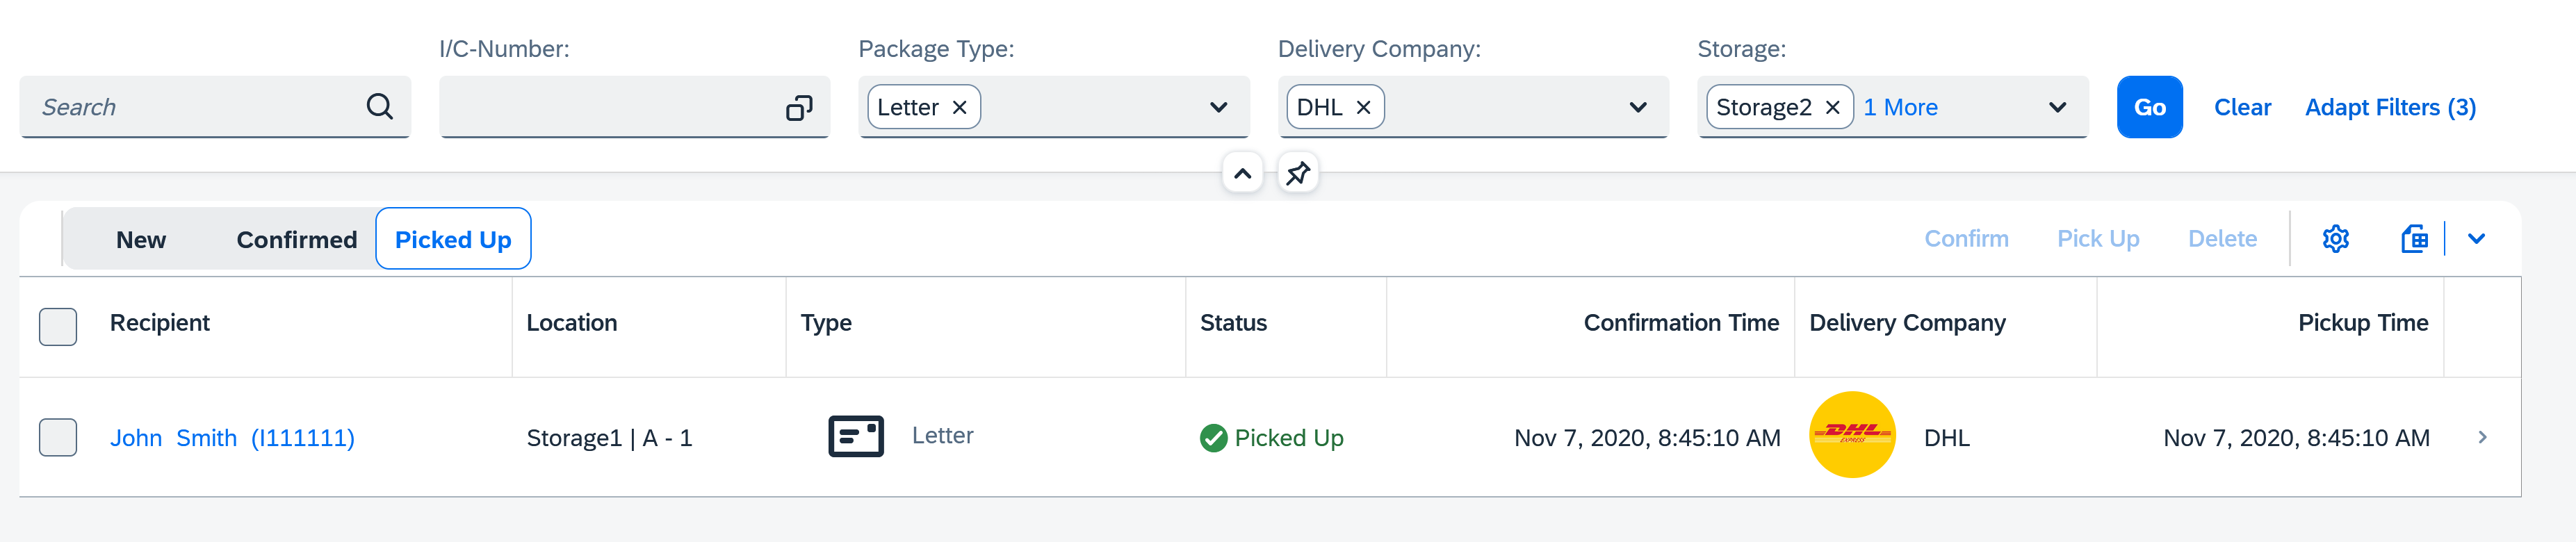
\includegraphics[width=0.45\linewidth]{images/user_doc/managePack/ReportScreen/browse/filterAfterGo.png}}
    \caption{Manage Package Report Screen - Adjust Filters}
    \label{fig:MPAjustFilters}
\end{figure}

In the middle there is a variant bread cum on the left and three action buttons on the right (\autoref{fig:MPMiddle}). The variant breadcrumb shows the three possible status of the packages. When clicking on one of the variants, the list of packages with corresponding status are displayed (\autoref{fig:MPbreadcrumbShowCase}, \autoref{fig:MPBreadCrumb}). The three action buttons are by default inactivated. They will be activated when certain conditions are full filled (i.e. the action can be performed).

\begin{figure}[H]
	\centering
	\subcaptionbox{Variants Bread}{
		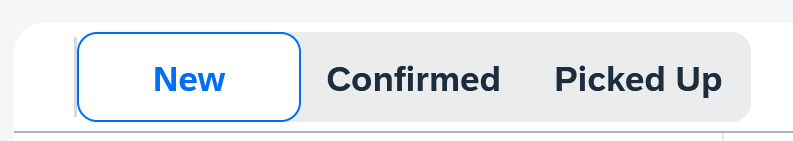
\includegraphics[width=0.45\linewidth]{images/user_doc/managePack/ReportScreen/browse/VariantsBread.png}}
	\hspace{5pt}
	\subcaptionbox{Action Buttons}{
		
\includegraphics[width=0.45\linewidth]{images/user_doc/managePack/ReportScreen/browse/buttonInactive.png}}
  \caption{Manage Packages Report Screen - Middle Control}
	\label{fig:MPMiddle}
\end{figure}

\begin{figure}[H]
	\centering
	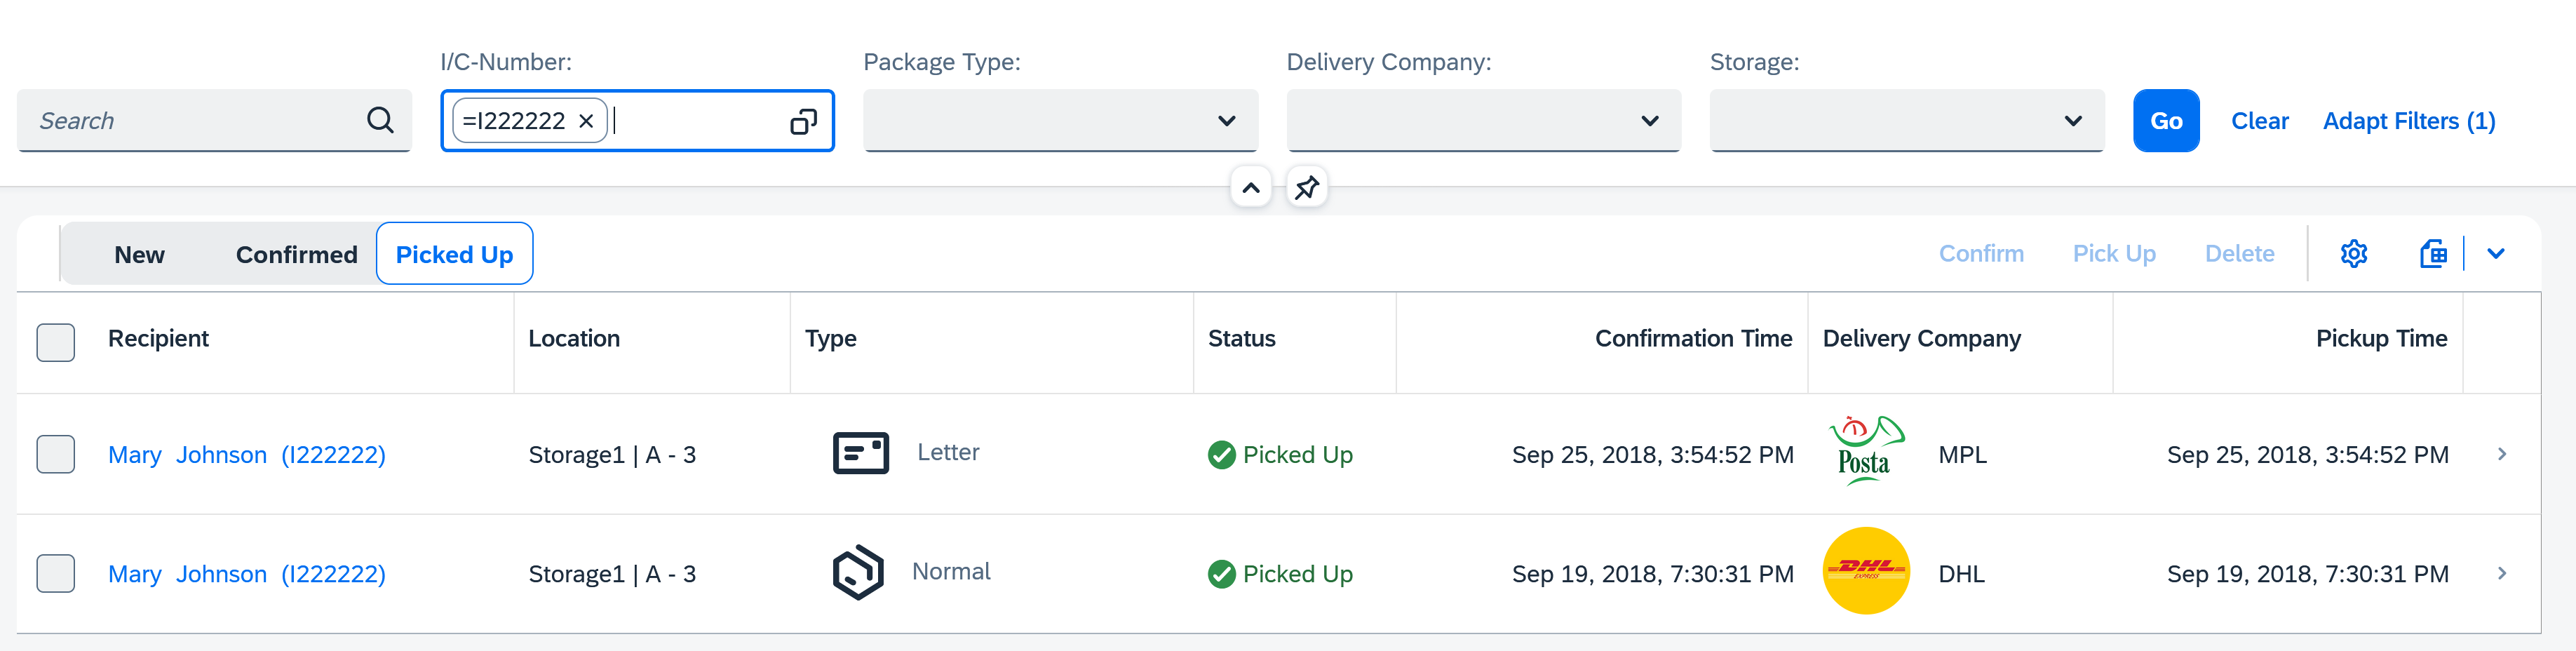
\includegraphics[width=1\linewidth]{images/user_doc/managePack/ReportScreen/browse/defaultFreeTextIdUsage.png}
	\caption{Manage Packages Report Screen - Middle Control - Breadcrumb Show Case}
	\label{fig:MPbreadcrumbShowCase}
\end{figure}


\begin{figure}[H]
	\centering
	\subcaptionbox{New Variant}{
		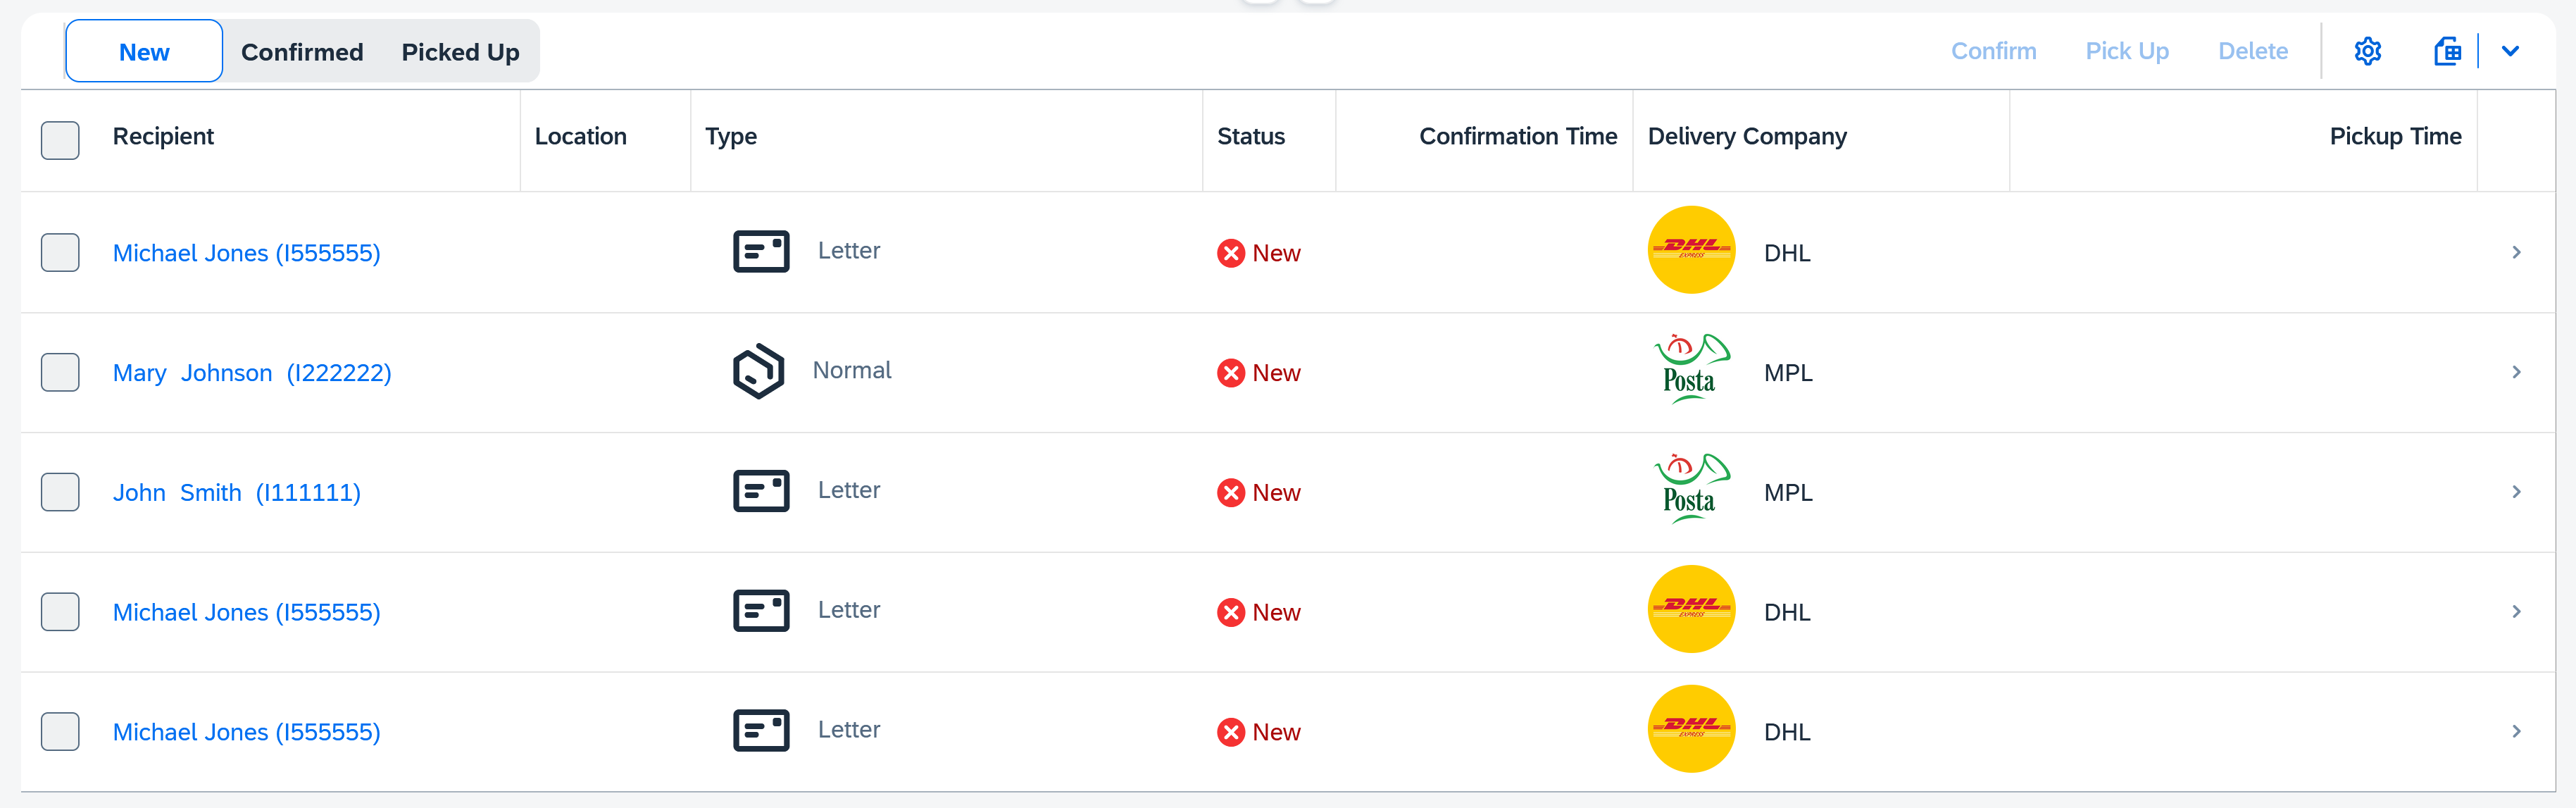
\includegraphics[width=0.45\linewidth]{images/user_doc/managePack/ReportScreen/browse/NewVariant.png}}
	\hspace{5pt}
	\subcaptionbox{Confirmed Variant}{
		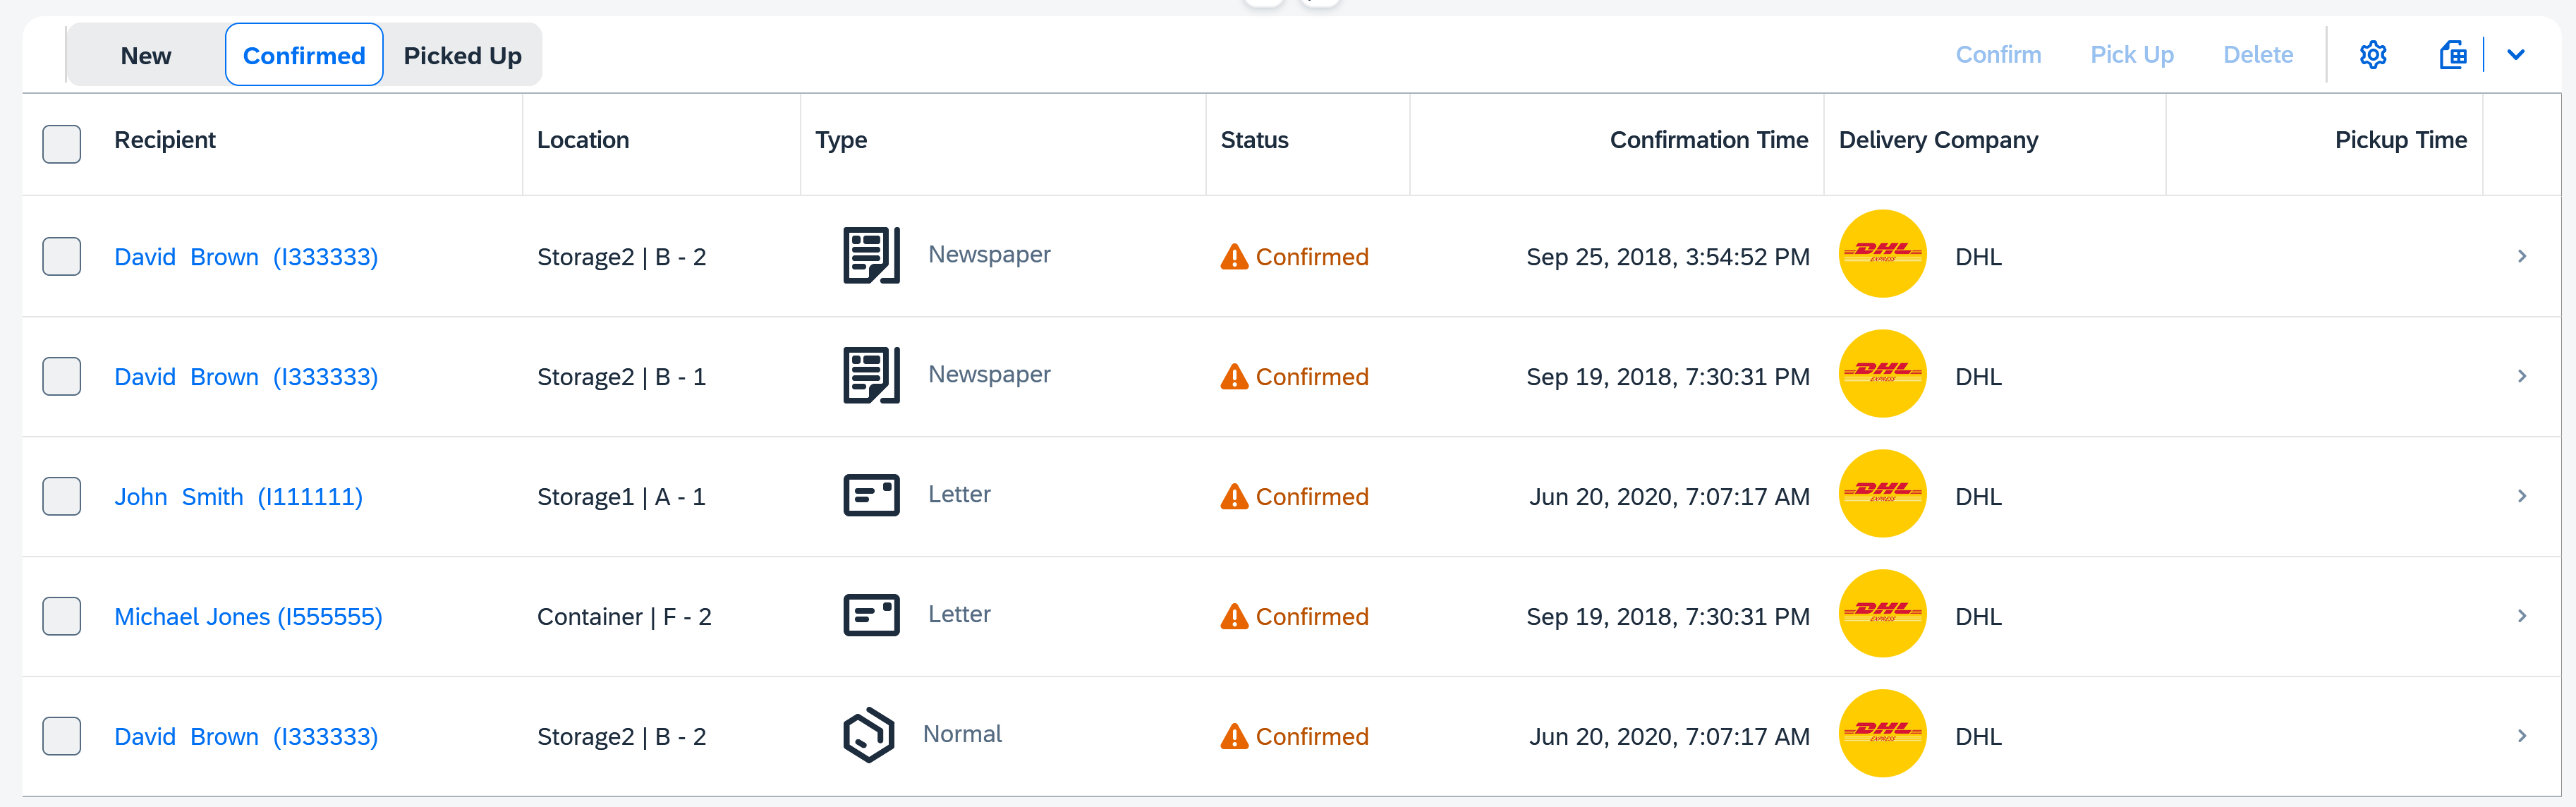
\includegraphics[width=0.45\linewidth]{images/user_doc/managePack/ReportScreen/browse/ConfirmedVariant.png}}

    \subcaptionbox{Picked Up Variant}{
		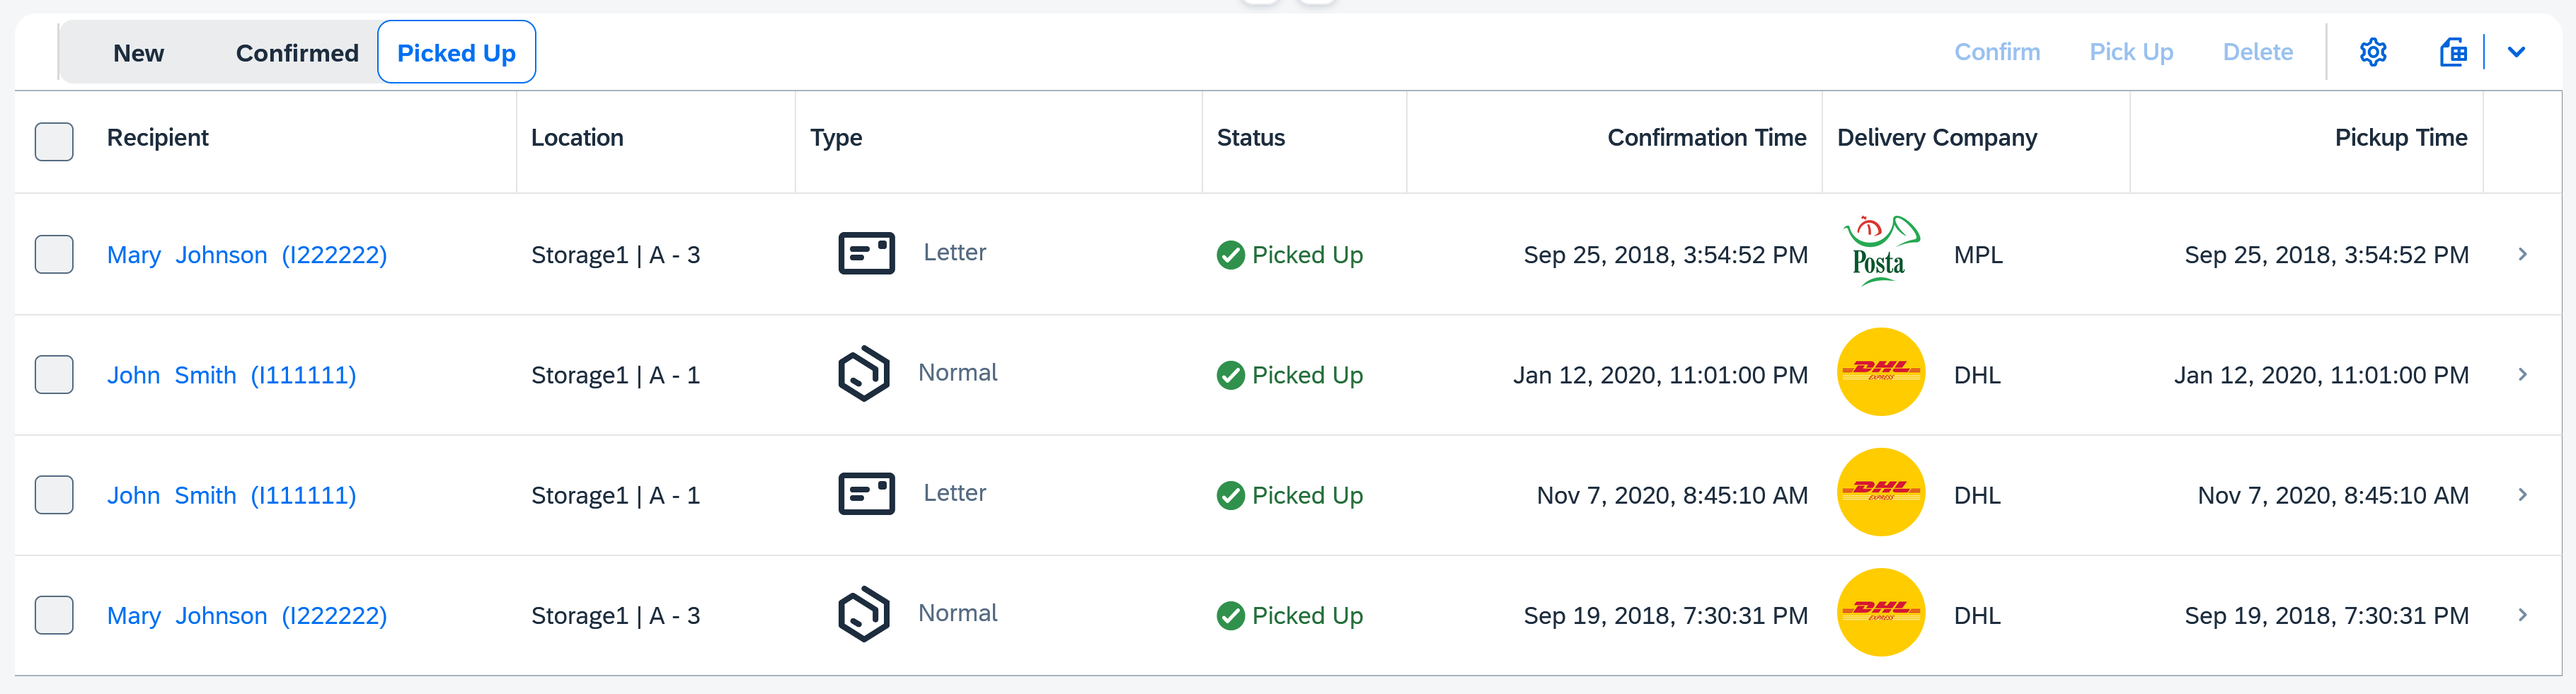
\includegraphics[width=0.45\linewidth]{images/user_doc/managePack/ReportScreen/browse/pickedupVariant.png}}
	\caption{Manage Packages Report Screen - Middle Control - Breadcrumb Show Case}
	\label{fig:MPBreadCrumb}
\end{figure}

The lower part displays the list of packages. The information provides for each packages are: \textbf{Recipient} (the recipient info, full name and SAP ID), \textbf{Location} (the storage and storage slot info of the package, if applicable), \textbf{Type} (the type of the package, existing types are newspaper, letter and normal), \textbf{Status} (the status of the package, existing status are new, confirmed and picked up), \textbf{Delivery Company} (the delivery company of the package), \textbf{Confirmation Time} (the confirmation time of the package, if applicable), \textbf{Pickup Time} (the picked up time of the package, if applicable).
In case selection of package is needed, one can select a package by ticking the selection box before the listed package item. One can also select and de-select all packages by toggling the selection box at the left corner of the list header (\autoref{fig:MPListSelection}).
In case contact info is needed for certain recipient, one can click at the \textbf{recipient}, a pop up contact card will display the email and phone number of the recipient (\autoref{fig:MPReportCOntactCard}).

\begin{figure}[H]
	\centering
	\subcaptionbox{Select All}{
		\includegraphics[width=0.45\linewidth]{images/user_doc/managePack/ReportScreen/browse/listSelectAll.png}}
	\hspace{5pt}
	\subcaptionbox{Deselect All}{
		\includegraphics[width=0.45\linewidth]{images/user_doc/managePack/ReportScreen/browse/listDeSelectAll.png}}
    \caption{Manage Packages Report Screen - Report List - Selection Show Case}
	\label{fig:MPListSelection}
\end{figure}

\begin{figure}[H]
	\centering
	\includegraphics[height=200pt]{images/user_doc/managePack/ReportScreen/browse/contactcard.png}
	\caption{Manage Packages Report Screen - Report List - Contact Card Show Case}
	\label{fig:MPReportCOntactCard}
\end{figure}

Further details of a package can be obtained by clicking at the package list items. On click, one is navigated to the "Package Detail Screen" displaying \textbf{Basic}, \textbf{General Data} and \textbf{Administrative Data} of the package. (\autoref{fig:MPdetailOverview})

In case the contact info of recipient or receptionist is needed, a contact card can be displayed by clicking on the person. (\autoref{fig:MPObjectContactCard})

\begin{figure}[H]
	\centering
	\includegraphics[height=200pt]{images/user_doc/managePack/DetailScreen/browse/overview.png}
	\caption{Manage Packages Detail Screen - Overview}
	\label{fig:MPdetailOverview}
\end{figure}

\begin{figure}[H]
	\centering
	\subcaptionbox{Receptionist}{
		\includegraphics[width=0.45\linewidth]{images/user_doc/managePack/DetailScreen/browse/contactcard_recep.png}}
	\hspace{5pt}
	\subcaptionbox{Recipient}{
		\includegraphics[width=0.45\linewidth]{images/user_doc/managePack/DetailScreen/browse/contactcard_user.png}}
    \caption{Manage Packages Detail Screen - Contact Card}
	\label{fig:MPObjectContactCard}
\end{figure}

\subsubsection{Confirm Packages}

Confirm a package happens after a \textbf{Receptionist} registered a delivered package when the \textbf{Receptionist} would like to allocate the package a storage slot. Only packages with \textit{new} status can be confirmed. One to many \textit{new} packages can be confirmed at a single time.

The \textbf{Confirm} button at the middle control part is used to trigger the confirm action. It is inactivated until the following conditions are all full filled:

\begin{compactenum}
    \item At the \textbf{New} variant.
    \item At least one \textit{new} package is selected.
\end{compactenum}

\bigskip
Once the \textbf{Receptionist} selected the packages (\autoref{fig:MPReportConfirmBtn}), the \textbf{Confirm} button is activated and clicked, a dialog pops up for the \textbf{Receptionist} to allocate a slot for the package(s) (\autoref{fig:MPReportConfirmDlg}). One should select the storage first from the \textbf{Storage} drop down list and then the slot from the \textbf{Slot} drop down list. The \textbf{Slot} drop down shows always the available slots under the selected storage (\autoref{fig:MPReportConfirmDlgSelection}).

After selected the slot, if one clicks "Close", nothing will happen and dialog will be closed. If one clicks "Save", the packages will be confirmed (i.e. filled with the selected slot info and status changed to confirmed). The dialog will be closed, a message toast indicates the success confirm and the package(s) will be moved from the current \textbf{New} variant to \textbf{Confirmed} Variant. (\autoref{fig:MPReportConfirmDlgButton})

At this point, the package(s) are ready to be picked up, by employee through \textbf{Package Pickup} (\autoref{subsec:pp}) application or by \textbf{Receptionist} using the pickup backup function (\autoref{subsubsec:MPpickup}) of this application.

\bigskip
Note that the confirm action is not irreversible, i.e. a \textit{confirmed} package can no longer be reset to \textit{new} and the confirmed package location can no longer be changed.

\begin{figure}[H]
	\centering
	\includegraphics[width=1\linewidth]{images/user_doc/managePack/ReportScreen/browse/confirmActivated.png}
	\caption{Manage Packages Report Screen - Confirm Step 1 - Select Packages}
	\label{fig:MPReportConfirmBtn}
\end{figure}

\begin{figure}[H]
	\centering
	\includegraphics[height=150pt]{images/user_doc/managePack/ReportScreen/confirm/confirmDialog.png}
	\caption{Manage Packages Report Screen - Confirm Step 2 - Confirm Dialog}
	\label{fig:MPReportConfirmDlg}
\end{figure}

\begin{figure}[H]
	\centering
	\subcaptionbox{Choose Storage}{
		\includegraphics[width=0.45\linewidth]{images/user_doc/managePack/ReportScreen/confirm/confirmStorageDropDown.png}}
	\hspace{5pt}
	\subcaptionbox{Choose Slot}{
		\includegraphics[width=0.45\linewidth]{images/user_doc/managePack/ReportScreen/confirm/confirmSlotDropdown.png}}
    \caption{Manage Packages Report Screen - Confirm Step 3 - Confirm Dialog - Location Selection}
	\label{fig:MPReportConfirmDlgSelection}
\end{figure}

\begin{figure}[H]
	\centering
	\subcaptionbox{Clicked "Save" and Proceeded}{
		\includegraphics[width=0.45\linewidth]{images/user_doc/managePack/ReportScreen/confirm/confirmedToast.png}}
	\hspace{5pt}
	\subcaptionbox{Clicked "Close" and Cancelled}{
		\includegraphics[width=0.45\linewidth]{images/user_doc/managePack/ReportScreen/browse/conifirmClosedClicked.png}}
    \caption{Manage Packages Report Screen - Confirm Step 4 - Confirmed / Cancelled}
	\label{fig:MPReportConfirmDlgButton}
\end{figure}

\subsubsection{Pickup Package}
\label{subsubsec:MPpickup}

Pickup a package happens when the recipients (package owners) came to the reception trying to pickup their confirmed packages and are unable to access the \textbf{Pickup Packages} application on their own. In this case a \textbf{Receptionist} may pickup the package in system on behalf of the recipients. Only packages with \textit{confirmed} status can be confirmed. Only one \textit{confirmed} package at one time can be pickup.

The \textbf{Pickup} button at the middle control part is used to trigger the pickup action. It is inactivated until all the following conditions are full filled:

\begin{compactenum}
    \item At the \textbf{Confirmed} variant.
    \item Exactly one \textit{confirmed} package is selected.
\end{compactenum}

\bigskip
Once the \textbf{Confirm} button is activated (\autoref{fig:MPReportPickupBtn}) and clicked, a warning message box (\autoref{fig:MPReportPickupDlg}) pops up verifying the \textbf{Receptionist}'s intention to mark a package as pickup. If one "OK" is clicked, the packages will be picked up (i.e. status is changed to pickup, all related processes are closed, package logs can no longer be removed from the system). The dialog will be closed, a message toast indicates the success pickup and the package will be moved from the current \textbf{Confirmed} variant to \textbf{Picked Up} Variant. (\autoref{fig:MPReportPickupDlgButton})

\bigskip
Note that the confirm action is not irreversible, i.e. a \textit{picked up} package can no longer be reset to \textit{confirm} or \textit{new}. However, the picked up package's information can still be modified (see \autoref{subsubsec:MPedit}).

\begin{figure}[H]
	\centering
	\includegraphics[width=1\linewidth]{images/user_doc/managePack/ReportScreen/pickup/pickupEnabled.png}
	\caption{Manage Packages Report Screen - Pickup Step 1 - Select Packages}
	\label{fig:MPReportPickupBtn}
\end{figure}

\begin{figure}[H]
	\centering
	\includegraphics[height=100pt]{images/user_doc/managePack/ReportScreen/pickup/pickupDialogOk.png}
	\caption{Manage Packages Pickup Dialog - Pickup Step 2}
	\label{fig:MPReportPickupDlg}
\end{figure}

\begin{figure}[H]
	\centering
	\subcaptionbox{Clicked "OK" and Proceeded}{
		\includegraphics[width=0.45\linewidth]{images/user_doc/managePack/ReportScreen/pickup/pickupToast.png}}
	\hspace{5pt}
	\subcaptionbox{Clicked "Cancel" and Cancelled}{
		\includegraphics[width=0.45\linewidth]{images/user_doc/managePack/ReportScreen/pickup/pickupCanceled.png}}
    \caption{Manage Packages Report Screen - Pickup Step 3 - Pickup / Cancelled}
	\label{fig:MPReportPickupDlgButton}
\end{figure}

\subsubsection{Delete Packages}

Delete a package can be done in two ways: Batch deletions at the "Report Screen" or single deletion at "Detail Screen". Only packages with \textit{confirmed} or \textit{new} status can be deleted. Packages with \textit{picked up} status can no longer be removed. Note that the deletion action is not irreversible.

\bigskip
In case the \textbf{Receptionist} is at "Report Screen" and want to delete one to many package, one can use the "Delete" button at the middle control bar. The "Delete" button is in activated until the following conditions are full filled:

\begin{compactenum}
    \item At the \textbf{Confirmed} or \textbf{New} variant.
    \item At least one package is selected.
\end{compactenum}

\bigskip
Once the \textbf{Delete} button is activated (\autoref{fig:MPReportDeleteBtn}) and clicked, a warning message box (\autoref{fig:MCReportDeleteDlg}) pops up verifying the \textbf{Receptionist}'s intention to delete a package. If one "OK" is clicked, the packages will be deleted (i.e. the package no longer exist in the system). The message box will be closed, a message toast indicates the success deletion and the package will be removed from everywhere. If "Cancel" is clicked, the message box is closed and nothing happens. (\autoref{fig:MPReportDeleteDone})

\begin{figure}[H]
	\centering
	\subcaptionbox{Enabled}{
		\includegraphics[width=0.95\linewidth]{images/user_doc/managePack/ReportScreen/delete/deleteEnabled.png}}

	\subcaptionbox{Disabled for Picked Up Packages}{
		\includegraphics[width=0.95\linewidth]{images/user_doc/managePack/ReportScreen/delete/deleteDisabled.png}}
    \caption{Manage Packages Report Screen - Delete Step 1 - Select Packages}
	\label{fig:MPReportDeleteBtn}
\end{figure}

\begin{figure}[H]
	\centering
	\includegraphics[height=100pt]{images/user_doc/managePack/ReportScreen/delete/deleteDlalog.png}
	\caption{Manage Packages Delete Dialog - Delete Step 2}
	\label{fig:MPReportDeleteDlg}
\end{figure}

\begin{figure}[H]
	\centering
	\includegraphics[height=100pt]{images/user_doc/managePack/ReportScreen/delete/deleteToast.png}
	\caption{Manage Packages Delete Dialog - Delete Step 3 - Deleted}
	\label{fig:MPReportDeleteDone}
\end{figure}


\bigskip
In case the \textbf{Receptionist} is at "Detail Screen" and want to delete the displayed package, the "Delete" button at the top right corner (page header) shall be used. 
The Delete" button is activated if the following conditions are full filled:

\begin{compactenum}
    \item The displayed package is in the status \textbf{new} or \textbf{confirmed}
\end{compactenum}

\bigskip
If the "Delete" button is activated and once clicked, a warning message box pops up verifying the \textbf{Receptionist}'s intention to delete the displayed package. If "Delete" is clicked, the packages will be deleted (i.e. the package no longer exist in the system). The message box will be closed, \textbf{Receptionist} got navigated back to "Report Screen" and a message toast indicates the success deletion. The package will be removed from everywhere. If "Cancel" is clicked, the message box is closed and nothing happens. (\autoref{fig:MPDetailDeleteGuide})

\begin{figure}[H]
	\centering
    \vspace{5pt}
	\subcaptionbox{Step 1: Deletion Enabled for Non-picked Up Packages}{
		\includegraphics[width=0.95\linewidth]{images/user_doc/managePack/DetailScreen/delete/deleteEnabled2.png}}
    \vspace{10pt}
	\subcaptionbox{Step 2: Deletion Verification}{
		\includegraphics[height=150pt]{images/user_doc/managePack/DetailScreen/delete/deleteDialog2.png}}
    \vspace{10pt}
    \subcaptionbox{Step 3: Navigated Back}{
		\includegraphics[width=1\linewidth]{images/user_doc/managePack/ReportScreen/delete/deleteToast.png}}
    \caption{Manage Packages Detail Screen - Delete Package Guide}
	\label{fig:MPDetailDeleteGuide}
\end{figure}

\subsubsection{Edit Package}
\label{subsubsec:MPedit}

Edit a package can be done at "Detail Screen".
In case the \textbf{Receptionist} is at "Detail Screen" and want to edit the displayed package, one can use the "Edit" button at top right corner (page header). 
When the "Edit" button is clicked, a editing dialog pops up, allowing \textbf{Receptionist} to modified the \textbf{Recipient}, \textbf{Type}, \textbf{Delivery Company}, \textbf{Comment} of the package. (\autoref{fig:MPDetailEditBtn})
When click "Save", the modified details are submitted, the dialog closes, a message toast pops up indicating the success and the changes reflects ont the "Detail Screen". When click "Close", any changes will be discard, the dialog simply closes.
(\autoref{fig:MPReportEditDone}

\begin{figure}[H]
	\centering
    \vspace{5pt}
	\subcaptionbox{Step 1: Edit Dialog}{
		\includegraphics[width=0.45\linewidth]{images/user_doc/managePack/DetailScreen/edit/editDialog.png}}
    \hspace{5pt}
    \subcaptionbox{Step 2: Modify Recipient}{
		\includegraphics[width=0.45\linewidth]{images/user_doc/managePack/DetailScreen/edit/editSelection1.png}}
	\subcaptionbox{Step 3: Modify Type}{
		\includegraphics[width=0.45\linewidth]{images/user_doc/managePack/DetailScreen/edit/editSelection2.png}}
    \hspace{5pt}
    \subcaptionbox{Step 4: Modify Delivery Company}{
		\includegraphics[width=0.45\linewidth]{images/user_doc/managePack/DetailScreen/edit/editSelection3.png}}
    \caption{Manage Packages Detail Screen - Edit Dialog Guide}
	\label{fig:MPDetailEditBtn}
\end{figure}


\begin{figure}[H]
	\centering
	\includegraphics[width=1\linewidth]{images/user_doc/managePack/DetailScreen/edit/editToast.png}
	\caption{Manage Packages Detail Screen - Edited}
	\label{fig:MPReportEditDone}
\end{figure}

\pagebreak

\section{Facility Manager}
\label{sec:UdocFacilityManager}

As a logged in \textbf{Facility Manager} (See \autoref{sec:GeneralRequisite} for all possible roles, one is granted to access the two applications under the \textbf{Administration} section, namely \textbf{Manage Companies} (\autoref{subsec:mc}) and \textbf{Manage Storage} (\autoref{subsec:ms}). One can quick jump to the section by left clicking the "Administration" tab. One can enter the application by left click the tiles. (\autoref{fig:ManagerApplications})

\begin{figure}[H]
	\centering
	\includegraphics[width=1\linewidth]{images/user_doc/overviews/AdminTab.png}
	\caption{Facility Management Applications}
	\label{fig:ManagerApplications}
\end{figure}


\subsection{Manage Companies}
\label{subsec:mc}

The \textbf{Manage Companies} application is used by \textbf{Facility Manager} (in short \textbf{FM}) maintaining the information of potential delivery companies delivering the package in the system. For each delivery company, its name, optionally a logo and the administration data (creation time, creation user, last modified time, last modified user) are stored. The administration data are auto maintained and is not editable by the \textbf{FM}. The summarized main actions the \textbf{FM} can take within the application are listed here:

\begin{compactenum}
	\item Browse the delivery companies.
        \begin{compactenum}
            \item Filtering possibility.
            \item Report List of delivery companies info.
            \item Detail page for single delivery company.
        \end{compactenum}
    \item Add new delivery companies. (name and logo)
    \item Edit existing delivery companies (name and logo).
    \item Delete package(s) which status is new or confirmed.
\end{compactenum}

\subsubsection{Browse}
As an \textbf{FM}, after clicking at the application tile, is redirected to the "Report Screen", which is the main screen of the application. (\autoref{fig:CompanyOverview})

\begin{figure}[H]
	\centering
	\includegraphics[width=1\linewidth]{images/user_doc/company/report/overview.png}
	\caption{Manage Companies - Overview}
	\label{fig:CompanyOverview}
\end{figure}

The upper part displays the search bar and the possible filters. 
In case the need of free text search of any possible content of the column, one can use the \textbf{"Search Bar"}. The search supports in-completed keywords and is case insensitive. One can also use the fixed filters for administration data. "Created By" and "Last Updated By" accepts free text of any valid SAP ID. "Created On" and "Last Updated On" requires entries of time stamps. \textbf{FM} can click at the double square at the right of input bar to open a filter help dialog, where specific criteria (e.g. between, equal, contains, etc.) can be chosen and a time entry clock can be used to enter time stamps. (\autoref{fig:CompanyOverview})

When adjusting the filtering values, the list view is temporarily locked. After adjusting the filtering values, one can run and review the filter result by clicking the "Go" button or hit "Enter" on keyboard. In case a company is edited and the table content is not reflected, click the "Go" button or hit "Enter" on keyboard to refresh. (\autoref{fig:CompanyOverview})

The lower part displays the list of delivery companies. In the list header, number of total delivery companies in the list is displayed on the left and two action buttons, "Create" and "Delete" are placed on the right. (\autoref{fig:CompanyOverview})

The information provides for each delivery companies in the list body (table) are: \textbf{Delivery Company} (company name with logo), \textbf{Created On} (the creation time of the company), \textbf{Created By} (the company creator's SAP ID). (\autoref{fig:CompanyOverview})

In case selection of package is needed, one can select a package by ticking the selection box before the listed package item. One can also de-select all packages by clicking at the selection box at the left corner of the table header. (\autoref{fig:CompanyOverview})

\bigskip

When the \textbf{FM} click at one item of the table, the \textbf{FM} is redirected to the "Detail Screen" displays the details of the selected item. (\autoref{fig:MCdetailOVerview})

\begin{figure}[H]
	\centering
	\includegraphics[width=1\linewidth]{images/user_doc/company/detail/DetailOverview.png}
	\caption{Manage Company Detail Screen - Overview}
	\label{fig:MCdetailOVerview}
\end{figure}

The "Detail Screen" displays the company name as the title on the left and two action buttons, "Delete" and "Edit" at the right in the header, and its full administration data in the body. (\autoref{fig:MCdetailOVerview})

\subsubsection{Add}

\textbf{FM} can add new delivery company to the system at "Report Screen" by clicking the "Create" button. 
When the "Create" button is clicked, a creation dialog pops up, where the \textbf{Name} and the \textbf{Logo} info of the company should be entered. The \textbf{Name} waits for input of free text of the company name and should not be left empty. The \textbf{Logo} waits for input of free text of a url to the image of the company's logo and can be left empty. (\autoref{fig:MCreportCreateGuide} - a,b)

After filling the dialog form, if "Create" is clicked, the entered info will be submitted, the dialog will be closed, a success message toast is displayed and the entered company appears in the table on the "Report Screen". If "Cancel" is clicked, the dialog will be closed, entered data is discarded and nothing happens. (\autoref{fig:MCreportCreateGuide} - c)

\begin{figure}[H]
	\centering
	\subcaptionbox{Step 1: Create Dialog}{
		\includegraphics[width=0.45\linewidth]{images/user_doc/company/report/createDlg.png}}
    \hspace{5pt}
    \subcaptionbox{Step 2: Data Entry}{
		\includegraphics[width=0.45\linewidth]{images/user_doc/company/report/createDlgEntries.png}}
    \vspace{10pt}
   \subcaptionbox{Step 3: Post Creation}{
		\includegraphics[width=1\linewidth]{images/user_doc/company/report/createdToast.png}}
    \caption{Manage Company Report Screen - Create Dialog Guide}
	\label{fig:MCreportCreateGuide}
\end{figure}

\subsubsection{Edit Company}

Edit a delivery company can be done at "Detail Screen" by the \textbf{FM}.
\bigskip

In case the \textbf{FM} is at "Detail Screen" and want to edit the displayed company, the \textbf{FM} can use the "Edit" button at top right corner (page header). 
When the "Edit" button is clicked, a editing dialog pops up, allowing \textbf{FM} to modified the \textbf{Name}, \textbf{Logo} of the company. Initially the fields are filled with current data of the company. The \textbf{Name} should contain free text of the company's name and should not be left empty. The \textbf{Logo} should contain free text of a url to the logo image and can be left empty.
When click "Save", the modified details are submitted, the dialog closes, a message toast pops up indicating the success and the changes reflects on the "Detail Screen". When click "Close", any changes will be discard, the dialog simply closes. (\autoref{fig:MCDetailEditGuide}, \autoref{fig:MCDetailEditDlgBad})

\begin{figure}[H]
	\centering
    \vspace{5pt}
	\subcaptionbox{Step 1: Edit Dialog}{
		\includegraphics[width=0.35\linewidth]{images/user_doc/company/detail/EditDlg.png}}
    \hspace{5pt}
    \subcaptionbox{Step 2: Post Success Edit}{
		\includegraphics[width=0.55\linewidth]{images/user_doc/company/detail/EditToast.png}}
    \caption{Manage Company Detail Screen - Edit Dialog Guide}
	\label{fig:MCDetailEditGuide}
\end{figure}

\begin{figure}[H]
	\centering
    \vspace{5pt}
	\subcaptionbox{Empty Company Name}{
		\includegraphics[width=0.35\linewidth]{images/user_doc/company/detail/EditBadInput.png}}
    \hspace{5pt}
    \subcaptionbox{Step 2: Error Message}{
		\includegraphics[width=0.55\linewidth]{images/user_doc/company/detail/editBadInputErrorMsg.png}}
    \caption{Manage Companies Detail Screen - Edit Dialog - Bad Inputs Example}
	\label{fig:MCDetailEditDlgBad}
\end{figure}

\subsubsection{Delete Company}

Delete an existing delivery company can be done in two ways: Batch deletions at the "Report Screen" or single deletion at "Detail Screen". The deletion of a company implies that, the delivery company will be removed completely and any association of existing packages to this company is automatically removed as well. This means those packages will no longer holds any company information. The deletion action is irreversible. 

In case the \textbf{FM} is at "Report Screen" and want to delete one to many companies, one can use the "Delete" button at the list header. The "Delete" button is inactivated until the following conditions are full filled:

\begin{compactenum}
    \item At least one delivery company is selected.
\end{compactenum}

Once the \textbf{Delete} button is activated and clicked, a warning message box pops up verifying the \textbf{FM}'s intention to delete a package. If "OK" is clicked, the company(s) will be deleted. The message box will be closed, a message toast indicates the success deletion and the package will be removed from everywhere. If "Cancel" is clicked, the message box is closed and nothing happens.
(\autoref{fig:MCReportDeleteStep1}, \autoref{fig:MCReportDeleteDlg}, 
\autoref{fig:MCReportDeleteStep3})

\begin{figure}[H]
	\centering
	\includegraphics[width=0.90\linewidth]{images/user_doc/company/report/deleteBtnEnable.png}
	\caption{Manage Companies - Delete - Step 1: Select Company to Delete}
	\label{fig:MCReportDeleteStep1}
\end{figure}

\begin{figure}[H]
	\centering
	\includegraphics[height=100pt]{images/user_doc/company/report/deleteConfirmaton2.png}
	\caption{Manage Companies - Delete - Step 2: Delete Dialog}
	\label{fig:MCReportDeleteDlg}
\end{figure}

\begin{figure}[H]
	\centering
	\includegraphics[width=0.90\linewidth]{images/user_doc/company/report/deleteToast.png}
	\caption{Manage Companies - Delete - Step 3: Post Delete}
	\label{fig:MCReportDeleteStep3}
\end{figure}

\bigskip
In case the \textbf{FM} is at "Detail Screen" and want to delete the displayed company, the "Delete" button at the top right corner (page header) shall be used. 

Once clicked, a warning message box pops up verifying the \textbf{FM}'s intention to delete the displayed company. If "Delete" is clicked, the company will be deleted. The message box will be closed, \textbf{FM} got navigated back to "Report Screen" and a message toast indicates the success deletion. If "Cancel" is clicked, the message box is closed and nothing happens. (\autoref{fig:MCDetailDeleteGuide})

\begin{figure}[H]
	\centering
	\subcaptionbox{Step 1: Deletion Verification When Clicked "Delete"}{
		\includegraphics[height=150pt]{images/user_doc/company/detail/deleteConfirmation.png}}
    \vspace{10pt}
	\subcaptionbox{Step 2: Navigated Back After Deletion}{
		\includegraphics[width=1\linewidth]{images/user_doc/company/detail/AfterDeletionBack.png}}
    \caption{Manage Companies Detail Screen - Delete Company Guide}
	\label{fig:MCDetailDeleteGuide}
\end{figure}



\subsection{Manage Storage}
\label{subsec:ms}

The \textbf{Manage Storage} application is used by \textbf{Facility Manager} (in short \textbf{FM}) maintaining the information of potential storage places and storage slots within certain storage holding the package in the system.  
The summarized main actions the \textbf{FM} can take within the application are listed here:

\begin{compactenum}
	\item Browse the storage and slots in the storage.
        \begin{compactenum}
            \item Filtering possibility.
            \item Report List of storage.
            \item Detail page for storage.
            \item Detail page for slot.
        \end{compactenum}
    \item Add new storage.
        \begin{compactenum}
            \item At Storage Report Page.
        \end{compactenum}
    \item Edit existing storage.
        \begin{compactenum}
            \item At Storage Detail Page.
        \end{compactenum}
    \item Delete existing storage.
        \begin{compactenum}
            \item At Storage Report Page.
            \item At Storage Detail Page.
        \end{compactenum}
    \item Add new storage slot.
        \begin{compactenum}
            \item At Storage Detail Page.
        \end{compactenum}
    \item Batch add new storage slots.
        \begin{compactenum}
            \item At Storage Detail Page.
        \end{compactenum}
    \item Edit existing storage slot.
        \begin{compactenum}
            \item At Slot Detail Page.
        \end{compactenum}
    \item Delete existing storage slot.
        \begin{compactenum}
            \item At Slot Detail Page.
            \item At Storage Detail Page.
        \end{compactenum}
\end{compactenum}

\subsubsection{Browse}

As an \textbf{FM}, after clicking at the application tile, is redirected to the "Storage Report Screen", which is the main screen of the application. (\autoref{fig:MSstorageReportPage})

\begin{figure}[H]
	\centering
	\includegraphics[width=1\linewidth]{images/user_doc/storage/StorageReportPage/reportDefaultOverview.png}
	\caption{Manage Storage - Storage Report Screen}
	\label{fig:MSstorageReportPage}
\end{figure}

The upper part displays the search bar and the possible filters. 
In case the need of free text search of any possible content of the column, one can use the \textbf{"Search Bar"}. The search supports in-completed keywords and is case insensitive. 
\textbf{FM} can also use the default filters, "Building Floor" and "Building", which are two drop down of all available building floors and buildings. \textbf{FM} may use the "Adapt Filter" option (right most of the filter bar), through which \textbf{FM} can add more filters options onto the filter bar.
(\autoref{fig:MSstReportFilterBar}, 
\autoref{fig:MSstorageReportFilterDefault}, 
\autoref{fig:MSstorageReportFilterAdaption})

\begin{figure}[H]
	\centering
	\includegraphics[width=1\linewidth]{images/user_doc/storage/StorageReportPage/reportFilterBar.png}
	\caption{Manage Storage Storage Report Screen - Filter Bar}
	\label{fig:MSstReportFilterBar}
\end{figure}

\begin{figure}[H]
	\centering
	\subcaptionbox{Drop Down of All Possible Building Floor Options}{
		\includegraphics[width=0.45\linewidth]{images/user_doc/storage/StorageReportPage/defaultFIlterBF.png}}
    \hspace{5pt}
    \subcaptionbox{Drop Down of All Possible Building Options}{
		\includegraphics[width=0.45\linewidth]{images/user_doc/storage/StorageReportPage/defaultFIlterBD.png}}
    \caption{Manage Storage Storage Report Screen - Filter Drop down Show Case}
	\label{fig:MSstorageReportFilterDefault}
\end{figure}

\begin{figure}[H]
	\centering
	\subcaptionbox{Option Dialog 1: Simple List}{
		\includegraphics[width=0.45\linewidth]{images/user_doc/storage/StorageReportPage/filterOption.png}}
    \hspace{5pt}
    \subcaptionbox{Option Dialog 2: Grouped}{
		\includegraphics[width=0.45\linewidth]{images/user_doc/storage/StorageReportPage/filterOption2.png}}

    \vspace{10pt}
	\subcaptionbox{After Filter Adaption}{
		\includegraphics[width=1\linewidth]{images/user_doc/storage/StorageReportPage/filterAdaption.png}}
    \caption{Manage Storage Storage Report Screen - Filter Adaption Guide}
	\label{fig:MSstorageReportFilterAdaption}
\end{figure}

When adjusting the filtering values, the list view is temporarily locked. After adjusting the filtering values, one can run and review the filter result by clicking the "Go" button or hit "Enter" on keyboard. In case a storage is edited or deleted and the table content is not reflected, click the "Go" button or hit "Enter" on keyboard to refresh and get the freshest storage info. 
(\autoref{fig:MSstorageReportFilterLock})

\begin{figure}[H]
	\centering
    \vspace{5pt}
	\subcaptionbox{While Adjusting the Filters the Storage List is Locked}{
		\includegraphics[width=0.45\linewidth]{images/user_doc/storage/StorageReportPage/listLock.png}}
    \hspace{5pt}
    \subcaptionbox{Clicked "Go" to Display the Filtering Results}{
		\includegraphics[width=0.45\linewidth]{images/user_doc/storage/StorageReportPage/filterAfterGo.png}}
    \caption{Manage Storage Storage Report Screen - Filter Lock}
	\label{fig:MSstorageReportFilterLock}
\end{figure}

\bigskip

The lower part displays the list report of storage. In the list header, number of total storage in the list is displayed on the left and two action buttons, "Create" and "Delete", and a table column "setting" (icon) are placed on the right. (\autoref{fig:MSrl})

The default columns provides for each storage in the list body (table) are: \textbf{Name} (storage name), \textbf{Location} (the building floor the storage located on), \textbf{Location Instructions} (any helping info regarding the location of the storage), \textbf{Total Number of Packages} (the total number of the packages that had been confirmed in this storage since its creation), \textbf{Current Utilizations} (the number of packages that are currently confirmed in this storage), \textbf{Map} (a link, on click opens a new tab to the map of the location of the storage). 
(\autoref{fig:MSrl})

\textbf{FM} may add more columns to the table by clicking the "setting" icon on the list header. A column adaption dialog will pop up for the \textbf{FM} to select the columns to show.
(\autoref{fig:MSstorageReportColumnAdaption})

\begin{figure}[H] % Storage List
	\centering
	\includegraphics[width=1\linewidth]{images/user_doc/storage/StorageReportPage/reportList.png}
	\caption{Manage Storage Storage Report Screen - Storage List}
	\label{fig:MSrl}
\end{figure}

\begin{figure}[H] % MSstorageReportColumnAdaption
	\centering
	\subcaptionbox{Step 1: column "setting"}{
		\includegraphics[width=0.45\linewidth]{images/user_doc/storage/StorageReportPage/columnSettings.png}}
    \hspace{5pt}
	\subcaptionbox{Step 2: Column Selection Dialog}{
		\includegraphics[width=0.45\linewidth]{images/user_doc/storage/StorageReportPage/columnAdaptionDlg.png}}
    
    \vspace{10pt}
    \subcaptionbox{Step 3: Selected Columns Displayed}{
        \includegraphics[width=0.95\linewidth]{images/user_doc/storage/StorageReportPage/columnMOre.png}}
    \caption{Manage Storage Storage Report Screen - Column Adaption Guide}
	\label{fig:MSstorageReportColumnAdaption}
\end{figure}

In case selection of storage is needed, \textbf{FM} can select a package by ticking the selection box before the listed storage item. One can also deselect all storage by clicking at the selection box at the left corner of the table header.

\bigskip

When the \textbf{FM} click at one item of the table, the \textbf{FM} is redirected to the "Storage Detail Screen".
(\autoref{fig:MSdetailOVerview})

\begin{figure}[H]
	\centering
	\includegraphics[width=1\linewidth]{images/user_doc/storage/StorageReportPage/storageObjWithSlots.png}
	\caption{Manage Storage Storage Detail Screen - Overview}
	\label{fig:MSdetailOVerview}
\end{figure}

The header part of "Storage Detail Screen" displays the storage name as the title and location instruction as description on the left and two action buttons, "Delete" and "Edit" at the right.
Under the title it displays important info of the storage (location, total utilization, current utilization and map). On click the map, the \textbf{FM} will be redirected out of the application to the map of the storage.
(\autoref{fig:MSstorageObjHeader})

\begin{figure}[H] % StorageObjHeader
	\centering
	\includegraphics[width=1\linewidth]{images/user_doc/storage/StorageObjectPage/StorageObjHeader.png}
	\caption{Manage Storage Storage Detail Screen - Header}
	\label{fig:MSstorageObjHeader}
\end{figure}

The bottom body part displays the list of slots contained by the given storage. The list of slots displays the following columns / information: \textbf{Name} (slot name), \textbf{Total Number of Packages} (total number of the packages stored in the slot since its creation date), \textbf{status} (the status of the slot). The availiable status of the slot are: inuse (indicates there is currently at least one package stored inside), empty (indicates there is no package inside) and unavailable (indicates the slot cannot be used due to some reasons).
(\autoref{fig:MSstorageObjSlotList})

\begin{figure}[H] % slotList
	\centering
	\includegraphics[width=1\linewidth]{images/user_doc/storage/StorageObjectPage/slotList.png}
	\caption{Manage Storage Storage Detail Screen - Slot List}
	\label{fig:MSstorageObjSlotList}
\end{figure}

\bigskip

When the \textbf{FM} clicks on one slot item in the slot list, the \textbf{FM} is redirected to slot's "Slot Detail Page". 
(\autoref{fig:MSslotObjOverview})

\begin{figure}[H] % slotObjOverview
	\centering
	\includegraphics[width=1\linewidth]{images/user_doc/storage/SlotObjectPage/slotObjOverview.png}
	\caption{Manage Storage Slot Detail Screen}
	\label{fig:MSslotObjOverview}
\end{figure}


\subsubsection{Add Storage}

\textbf{FM} can add new storage to the system at "Report Screen" by clicking the "Create" button.
When the "Create" button is clicked, a creation dialog pops up. The \textbf{Name} waits for input of free text of the storage and should not be left empty. The \textbf{Map} waits for input of free text of a url to the location of the storage and can be left empty. The \textbf{Location Instruction} waits for input of free text and can be left empty.
(\autoref{fig:MSreportCreateGuide})

After filling the dialog form, if "Create" is clicked, the entered info will be submitted, the dialog will be closed, a success message toast is displayed and the entered storage appears in the table on the "Report Screen". If "Cancel" is clicked, the dialog will be closed, entered data is discarded and nothing happens.
(\autoref{fig:MSreportCreateGuide})

\begin{figure}[H]
	\centering
	\subcaptionbox{Step 1: Open Create Dialog}{
		\includegraphics[width=0.45\linewidth]{images/user_doc/storage/StorageReportPage/createStorageDlg.png}}
    \hspace{5pt}
    \subcaptionbox{Step 2.1: Data Entry - Select Building Floor}{
		\includegraphics[width=0.45\linewidth]{images/user_doc/storage/StorageReportPage/csdlgDropDown.png}}
  
    \vspace{10pt}
    \subcaptionbox{Step 2.2: Data Entry - Bad Input Warning Example}{
		\includegraphics[width=0.45\linewidth]{images/user_doc/storage/StorageReportPage/csdlgBadInput.png}}
    \hspace{5pt}
    \subcaptionbox{Step 2.2: Data Entry - Filled}{
		\includegraphics[width=0.45\linewidth]{images/user_doc/storage/StorageReportPage/csdlgFilled.png}}

    \vspace{10pt}
    \subcaptionbox{Step 3: Post Creation}{
		\includegraphics[width=1\linewidth]{images/user_doc/storage/StorageReportPage/createdToast.png}}
    
    \caption{Manage Storage Storage Report Screen - Create Storage Dialog Guide}
	\label{fig:MSreportCreateGuide}
\end{figure}


\subsubsection{Edit Storage}

\textbf{FM} can edit a storage at "Storage Detail Screen".
In case the \textbf{FM} is at "Storage Detail Screen" and want to edit the displayed company, the \textbf{FM} can use the "Edit" button at top right corner (page header). 
When the "Edit" button is clicked, a editing dialog pops up, allowing \textbf{FM} to modified the \textbf{Name}, \textbf{Building Floor}, \textbf{Map}, \textbf{Location Instructions} of the company. Initially the fields are filled with current data of the storage. The entry rules are the same as creating the storage.
When click "Save", the modified details are submitted, the dialog closes, a message toast pops up indicating the success and the changes reflects on the "Storage Detail Screen". When click "Close", any changes will be discard, the dialog simply closes.
(\autoref{fig:MSDetailEditBtn})

\begin{figure}[H]
	\centering
    \vspace{5pt}
	\subcaptionbox{Step 1: Edit Dialog}{
		\includegraphics[width=0.30\linewidth]{images/user_doc/storage/StorageObjectPage/storageEditDlg.png}}
    \hspace{5pt}
    \subcaptionbox{Step 2: Post Success Edit}{
		\includegraphics[width=0.60\linewidth]{images/user_doc/storage/StorageObjectPage/storageEditedToast.png}}
    \caption{Manage Storage Storage Detail Screen - Edit Dialog Guide}
	\label{fig:MSDetailEditBtn}
\end{figure}

\subsubsection{Delete Storage}

\textbf{FM} can delete a storage in two ways: Batch deletions at the "Storage Report Screen" or single deletion at "Storage Detail Screen". 
The deletion of a storage implies that, the storage will be removed completely from the system. The deletion action is irreversible. 

In case the \textbf{FM} is at "Storage Report Screen" and want to delete one to many storage, the \textbf{FM} can use the "Delete" button at the list header. The "Delete" button is in activated until the following conditions are full filled:

\begin{compactenum}
    \item At least one storage is selected.
\end{compactenum}

Once the \textbf{Delete} button is activated and clicked, a warning message box pops up verifying the \textbf{FM}'s intention to delete a storage. If one "Delete" is clicked, the selected storage will be deleted. The message box will be closed, a message toast indicates the success deletion. If "Cancel" is clicked, the message box is closed and nothing happens.
(\autoref{fig:MSreportDeleteGuide})

\begin{figure}[H]
	\centering
	\subcaptionbox{Step 1: Select Storage}{
		\includegraphics[width=0.95\linewidth]{images/user_doc/storage/StorageReportPage/deleteEnable.png}}
  
    \vspace{10pt}
    
    \subcaptionbox{Step 2: Delete Verification}{
		\includegraphics[width=0.45\linewidth]{images/user_doc/storage/StorageReportPage/deleteVerification.png}}
  
    \vspace{10pt}
    
    \subcaptionbox{Step 3: Deleted}{
		\includegraphics[width=0.95\linewidth]{images/user_doc/storage/StorageReportPage/deleteToast.png}}

    \caption{Manage Storage Storage Report Screen - Delete Storage Guide}
	\label{fig:MSreportDeleteGuide}
\end{figure}


\bigskip
In case the \textbf{FM} is at "Storage Detail Screen" and want to delete the displayed storage, the "Delete" button at the top right corner (page header) shall be used. 

Once clicked, a warning message box pops up verifying the \textbf{FM}'s intention to delete the displayed storage. If "Delete" is clicked, the storage will be deleted. The message box will be closed, \textbf{FM} got navigated back to "Storage Report Screen" and a message toast indicates the success deletion. If "Cancel" is clicked, the message box is closed and nothing happens.
(\autoref{fig:MSobjDeleteGuide})

\begin{figure}[H]
	\centering
	\subcaptionbox{On Click "Delete" - Deletion Verification}{
		\includegraphics[width=0.95\linewidth]{images/user_doc/storage/StorageObjectPage/storageDeleteMsg.png}}

    \caption{Manage Storage Storage Detail Screen - Delete Storage Guide}
	\label{fig:MSobjDeleteGuide}
\end{figure}


\subsubsection{Add Storage Slot}

\textbf{FM} can add new storage slot to the system at "Storage Detail Screen" by clicking the "Create" button on the top right corner of the slot list.
When the "Create" button is clicked, a creation dialog pops up. The \textbf{Name} waits for input of free text of the storage slot and should not be left empty. The \textbf{Available} selection box sets if the slot will be in an unavailable status.
(\autoref{fig:MSobjCreateSlotGuide})

After filling the dialog form, if "Create" is clicked, the entered info will be submitted, the dialog will be closed, a success message toast is displayed and the entered storage slot appears in the table on the "Storage Detail Screen". In case \textbf{Available} is selected, the created slot will by default "empty", otherwise, it displays "unavailable". If "Cancel" is clicked, the dialog will be closed, entered data is discarded and nothing happens.
(\autoref{fig:MSobjCreateSlotGuide})

\begin{figure}[H]
	\centering
	\subcaptionbox{Step 1: Open Create Dialog}{
		\includegraphics[width=0.45\linewidth]{images/user_doc/storage/StorageObjectPage/createSlotDlg.png}}
    \hspace{10pt}
    \subcaptionbox{Step 2: Data Entry - Bad Input Warning Example}{
		\includegraphics[width=0.45\linewidth]{images/user_doc/storage/StorageObjectPage/createSlotBadInput.png}}
  
    \vspace{10pt}
    \subcaptionbox{Step 3: Post Creation}{
		\includegraphics[width=0.95\linewidth]{images/user_doc/storage/StorageObjectPage/createdSlotToast.png}}
    
    \caption{Manage Storage Storage Detail Screen - Create Slot Dialog Guide}
	\label{fig:MSobjCreateSlotGuide}
\end{figure}


\subsubsection{Batch Add Storage Slot}

\textbf{FM} can add multiple new storage slots in a matrix way to the system at "Storage Detail Screen" by clicking the "Mass Create" button on the top right corner of the slot list.
When the "Mass Create" button is clicked, a creation dialog pops up. The \textbf{Number of Rows} and \textbf{Number of Columns} waits for numeric integer inputs of desired number of rows and columns to create. The \textbf{Type of Row Identifiers} and \textbf{Type of Column Identifiers} has two options: Number and Letter, indicates how the created matrix of slot will be named (Row - Column). If "Letter" is selected then "A-Z" will be used, otherwise, "1-9". For example, an entry of (1, Letter, 2, Number) will create (A - 1, A - 2). The selection of row and column type should not be the same.
(\autoref{fig:MSobjmassCreateSlotGuide})

After filling the dialog form, if "Create" is clicked, the entered info will be submitted, the dialog will be closed, a success message toast is displayed and the created storage slots appear in the table on the "Storage Detail Screen". If "Cancel" is clicked, the dialog will be closed, entered data is discarded and nothing happens.
(\autoref{fig:MSobjmassCreateSlotGuide})

\begin{figure}[H] % MSobjmassCreateSlotGuide
	\centering
	\subcaptionbox{Step 1: Open Create Dialog}{
		\includegraphics[width=0.45\linewidth]{images/user_doc/storage/StorageObjectPage/masCreateDlg.png}}

    \vspace{10pt}
    \subcaptionbox{Step 2.1: Data Entry - Row Type Selection}{
		\includegraphics[width=0.45\linewidth]{images/user_doc/storage/StorageObjectPage/massCreateFilling1.png}}
    \hspace{5pt}
    \subcaptionbox{Step 2.2: Data Entry - Column Type Selection}{
		\includegraphics[width=0.45\linewidth]{images/user_doc/storage/StorageObjectPage/massCreateFilling2.png}}

    \vspace{10pt}
    \subcaptionbox{Step 2.1: Data Entry - Row Type Selection}{
		\includegraphics[width=0.90\linewidth]{images/user_doc/storage/StorageObjectPage/massCreateSuccessToast.png}}
    \caption{Manage Storage Storage Detail Screen - Mass Create Slot Dialog Guide}
	\label{fig:MSobjmassCreateSlotGuide}
\end{figure}


\subsubsection{Edit Storage Slot}
\textbf{FM} can edit a slot at "Slot Detail Screen".
In case the \textbf{FM} is at "Slot Detail Screen" and want to edit the displayed slot, the \textbf{FM} can use the "Edit" button at top right corner (page header). 
When the "Edit" button is clicked, a editing dialog pops up, allowing \textbf{FM} to modified the \textbf{Name}, \textbf{Available} of the slot. Initially the fields are filled with current data of the slot. The entry rules are the same as creating a single slot.
When click "Save", the modified details are submitted, the dialog closes, a message toast pops up indicating the success and the changes reflects on the "Storage Detail Screen". When click "Close", any changes will be discard, the dialog simply closes.
(\autoref{fig:MSSlotDetailEditBtn})

\begin{figure}[H]
	\centering
    \vspace{5pt}
	\subcaptionbox{Step 1: Edit Dialog}{
		\includegraphics[width=0.30\linewidth]{images/user_doc/storage/SlotObjectPage/editSlotDlg.png}}
    \hspace{5pt}
    \subcaptionbox{Step 2: Post Success Edit}{
		\includegraphics[width=0.60\linewidth]{images/user_doc/storage/SlotObjectPage/editedslotToast.png}}
    \caption{Manage Storage Slot Detail Screen - Edit Dialog Guide}
	\label{fig:MSSlotDetailEditBtn}
\end{figure}

\subsubsection{Delete Storage Slot}

\textbf{FM} can delete a storage slot at "Slot Detail Screen". 
The deletion of a storage slot implies that, the storage slot will be removed completely from the system. The deletion action is irreversible. 

In case the \textbf{FM} is at "Slot Detail Screen" and want to delete the displayed storage, the "Delete" button at the top right corner (page header) shall be used. 

Once clicked, a warning message box pops up verifying the \textbf{FM}'s intention to delete the displayed slot. If "Delete" is clicked, the storage will be deleted. The message box will be closed, \textbf{FM} got navigated back to "Storage Detail Screen" and a message toast indicates the success deletion. \textbf{FM} should refresh the page to see the slot disappears from the slot list. If "Cancel" is clicked, the message box is closed and nothing happens.
(\autoref{fig:MSslotObjDeleteGuide})

\begin{figure}[H]
	\centering
	\subcaptionbox{On Click "Delete" - Deletion Verification}{
		\includegraphics[width=0.50\linewidth]{images/user_doc/storage/SlotObjectPage/deleteSlotDlg.png}}

    \vspace{10pt}
    
    \subcaptionbox{Post Deletion - Navigated Back}{
		\includegraphics[width=0.95\linewidth]{images/user_doc/storage/SlotObjectPage/deletedSlotToast.png}}
    \caption{Manage Storage Slot Detail Screen - Delete Slot Guide}
	\label{fig:MSslotObjDeleteGuide}
\end{figure}


\pagebreak
\section{Administrator}
\label{sec:UdocAdministrator}

As a logged in \textbf{Administrator} (See \autoref{sec:GeneralRequisite} for all possible roles, one has access to all the 6 applications. By clicking at the section code, one can reference backward to dedicated sections depends on the needs. 

\begin{itemize}
    \item \ref{subsec:ph} My Packages
    \item \ref{subsec:pp} Pickup Packages
    \item \ref{subsec:rp} Register Packages
    \item \ref{subsec:mp} Manage Packages
    \item \ref{subsec:mc} Manage Companies
    \item \ref{subsec:ms} Manage Storage
\end{itemize}

\subsection*{Conclusion}

By the end this chapter, one should have gained a comprehensive understanding of the capability of the developed solution. In the coming \autoref{ch:impl}, the underlying implementations are unveiled, where the freshest information on how the solution is built is provided.